% Options for packages loaded elsewhere
\PassOptionsToPackage{unicode}{hyperref}
\PassOptionsToPackage{hyphens}{url}
%
\documentclass[
  12pt,
]{article}
\usepackage{amsmath,amssymb}
\usepackage{lmodern}
\usepackage{iftex}
\ifPDFTeX
  \usepackage[T1]{fontenc}
  \usepackage[utf8]{inputenc}
  \usepackage{textcomp} % provide euro and other symbols
\else % if luatex or xetex
  \usepackage{unicode-math}
  \defaultfontfeatures{Scale=MatchLowercase}
  \defaultfontfeatures[\rmfamily]{Ligatures=TeX,Scale=1}
\fi
% Use upquote if available, for straight quotes in verbatim environments
\IfFileExists{upquote.sty}{\usepackage{upquote}}{}
\IfFileExists{microtype.sty}{% use microtype if available
  \usepackage[]{microtype}
  \UseMicrotypeSet[protrusion]{basicmath} % disable protrusion for tt fonts
}{}
\makeatletter
\@ifundefined{KOMAClassName}{% if non-KOMA class
  \IfFileExists{parskip.sty}{%
    \usepackage{parskip}
  }{% else
    \setlength{\parindent}{0pt}
    \setlength{\parskip}{6pt plus 2pt minus 1pt}}
}{% if KOMA class
  \KOMAoptions{parskip=half}}
\makeatother
\usepackage{xcolor}
\IfFileExists{xurl.sty}{\usepackage{xurl}}{} % add URL line breaks if available
\IfFileExists{bookmark.sty}{\usepackage{bookmark}}{\usepackage{hyperref}}
\hypersetup{
  pdftitle={Factors affecting reliablity of state-space age-structured assessment models},
  pdfauthor={Timothy J. Miller1,2; Greg Britten3; Elizabeth N. Brooks2; Gavin Fay4; Alex Hansell2; Christopher M. Legault2; Chengxue Li2; Brandon Muffley5; Brian C. Stock6; John Wiedenmann7},
  hidelinks,
  pdfcreator={LaTeX via pandoc}}
\urlstyle{same} % disable monospaced font for URLs
\usepackage[margin=1in]{geometry}
\usepackage{graphicx}
\makeatletter
\def\maxwidth{\ifdim\Gin@nat@width>\linewidth\linewidth\else\Gin@nat@width\fi}
\def\maxheight{\ifdim\Gin@nat@height>\textheight\textheight\else\Gin@nat@height\fi}
\makeatother
% Scale images if necessary, so that they will not overflow the page
% margins by default, and it is still possible to overwrite the defaults
% using explicit options in \includegraphics[width, height, ...]{}
\setkeys{Gin}{width=\maxwidth,height=\maxheight,keepaspectratio}
% Set default figure placement to htbp
\makeatletter
\def\fps@figure{htbp}
\makeatother
\setlength{\emergencystretch}{3em} % prevent overfull lines
\providecommand{\tightlist}{%
  \setlength{\itemsep}{0pt}\setlength{\parskip}{0pt}}
\setcounter{secnumdepth}{5}
\newlength{\cslhangindent}
\setlength{\cslhangindent}{1.5em}
\newlength{\csllabelwidth}
\setlength{\csllabelwidth}{3em}
\newlength{\cslentryspacingunit} % times entry-spacing
\setlength{\cslentryspacingunit}{\parskip}
\newenvironment{CSLReferences}[2] % #1 hanging-ident, #2 entry spacing
 {% don't indent paragraphs
  \setlength{\parindent}{0pt}
  % turn on hanging indent if param 1 is 1
  \ifodd #1
  \let\oldpar\par
  \def\par{\hangindent=\cslhangindent\oldpar}
  \fi
  % set entry spacing
  \setlength{\parskip}{#2\cslentryspacingunit}
 }%
 {}
\usepackage{calc}
\newcommand{\CSLBlock}[1]{#1\hfill\break}
\newcommand{\CSLLeftMargin}[1]{\parbox[t]{\csllabelwidth}{#1}}
\newcommand{\CSLRightInline}[1]{\parbox[t]{\linewidth - \csllabelwidth}{#1}\break}
\newcommand{\CSLIndent}[1]{\hspace{\cslhangindent}#1}
\usepackage{url}
\usepackage{setspace}
%\singlespacing
%\onehalfspacing
\doublespacing
\usepackage{lineno}
\linenumbers
\usepackage[belowskip=0pt,aboveskip=0pt]{caption}
\usepackage{relsize}
\usepackage{float}
\usepackage{lscape}
\usepackage{longtable}
\usepackage{amsmath,rotating}
\usepackage[scanall]{psfrag}
\usepackage{bm}
\usepackage{caption,graphics}
\usepackage{graphicx}
\usepackage{sectsty}
\usepackage{color}
\usepackage{fancyhdr}
\usepackage{xspace}
\usepackage{textcomp}
\usepackage{upgreek}
\renewcommand\figurename{Fig.}
\captionsetup{labelsep=period, singlelinecheck=false}
\newcommand{\changesize}[1]{\fontsize{#1pt}{#1pt}\selectfont}
\renewcommand{\arraystretch}{1.5}
%\renewcommand\theadfont{}

\newcommand{\Fmsy}{\ensuremath{F_{\text{MSY}}}\xspace}
\newcommand{\Fspr}[1]{\ensuremath{F_{\text{{#1}\%}}}\xspace}
\newcommand{\afrb}{Alaska Fishery Research Bulletin\xspace}
\newcommand{\ajms}{African Journal of Marine Science\xspace}
\newcommand{\amb}{Advances in Marine Biology\xspace}
\newcommand{\bms}{Bulletin of Marine Science\xspace}
\newcommand{\bjssf}{Bulletin of the Japanese Society of Scientific Fisheries\xspace}
\newcommand{\cb}{Conservation Biology\xspace}
\newcommand{\cjfas}{Canadian Journal of Fisheries and Aquatic Sciences\xspace}
\newcommand{\ea}{Ecological Applications\xspace}
\newcommand{\eer}{Evolutionary Ecology Research\xspace}
\newcommand{\elet}{Ecology Letters\xspace}
\newcommand{\emod}{Ecological Modelling\xspace}
\newcommand{\ebf}{Environmental Biology of Fishes\xspace}
\newcommand{\ff}{Fish and Fisheries\xspace}
\newcommand{\fo}{Fisheries Oceanography\xspace}
\newcommand{\fr}{Fisheries Research\xspace}
\newcommand{\fb}{Fishery Bulletin\xspace}
\newcommand{\ijms}{ICES Journal of Marine Science\xspace}
\newcommand{\iccat}{Collective Volume of Scientific Papers ICCAT\xspace}
\newcommand{\jae}{Journal of Animal Ecology\xspace}
\newcommand{\jai}{Journal of Applied Ichthyology\xspace}
\newcommand{\jdc}{Journal Du Conseil International Pour L'exploration De La Mer\xspace}
\newcommand{\jdcp}{Journal Du Conseil Permanent International Pour L'exploration De La Mer\xspace}
\newcommand{\jembe}{Journal of Experimental Marine Biology and Ecology\xspace}
\newcommand{\jfb}{Journal of Fish Biology\xspace}
\newcommand{\jsr}{Journal of Sea Research\xspace}
\newcommand{\jtb}{Journal of Theoretical Biology\xspace}
\newcommand{\jfrbc}{Journal of the Fisheries Research Board of Canada\xspace}
\newcommand{\jnwafs}{Journal of Northwest Atlantic Fisheries Science\xspace}
\newcommand{\mcf}{Marine and Coastal Fisheries: Dynamics, Management, and Ecosystem Science\xspace}
\newcommand{\mb}{Marine Biology\xspace}
\newcommand{\meps}{Marine Ecology Progress Series\xspace}
\newcommand{\mfr}{Marine Fisheries Review\xspace}
\newcommand{\mpb}{Marine Pollution Bulletin\xspace}
\newcommand{\najfm}{North American Journal of Fisheries Management\xspace}
\newcommand{\nzjmfr}{New Zealand Journal of Marine and Freshwater Research\xspace}
\newcommand{\pnas}{Proceedings of the National Academy of Sciences USA\xspace}
\newcommand{\rpvrciemm}{Rapports et Proc\`es-Verbaux des R\'eunions. Conseil Internationale pour l'Exploration de la Mer\xspace}
\newcommand{\rpvrcpiemm}{Rapports et Proc\`es-Verbaux des R\'eunions. Conseil Permanent Internationale pour l'Exploration de la Mer\xspace}
\newcommand{\rfbf}{Reviews in Fish Biology and Fisheries\xspace}
\newcommand{\sajms}{South African Journal of Marine Science\xspace}
\newcommand{\tafs}{Transactions of the American Fisheries Society\xspace}

\newcommand{\anzjs}{Australian \& New Zealand Journal of Statistics\xspace}
\newcommand{\as}{Applied Statistics\xspace}
\newcommand{\csda}{Computational Statistics \& Data Analysis\xspace}
\newcommand{\ees}{Environmental and Ecological Statistics\xspace}
\newcommand{\jas}{Journal of Applied Statistics\xspace}
\newcommand{\jabes}{Journal of Agricultural, Biological, and Environmental Statistics\xspace}
\newcommand{\jasa}{Journal of the American Statistical Association\xspace}
\newcommand{\jrssb}{Journal of the Royal Statistical Society. Series B\xspace}
\newcommand{\sm}{Statistics in Medicine}

\usepackage{booktabs}
\usepackage{longtable}
\usepackage{array}
\usepackage{multirow}
\usepackage{wrapfig}
\usepackage{float}
\usepackage{colortbl}
\usepackage{pdflscape}
\usepackage{tabu}
\usepackage{threeparttable}
\usepackage{threeparttablex}
\usepackage[normalem]{ulem}
\usepackage{makecell}
\usepackage{xcolor}
\ifLuaTeX
  \usepackage{selnolig}  % disable illegal ligatures
\fi

\title{Factors affecting reliablity of state-space age-structured
assessment models}
\author{Timothy J. Miller\textsuperscript{1,2} \and Greg
Britten\textsuperscript{3} \and Elizabeth N.
Brooks\textsuperscript{2} \and Gavin Fay\textsuperscript{4} \and Alex
Hansell\textsuperscript{2} \and Christopher M.
Legault\textsuperscript{2} \and Chengxue
Li\textsuperscript{2} \and Brandon Muffley\textsuperscript{5} \and Brian
C. Stock\textsuperscript{6} \and John Wiedenmann\textsuperscript{7}}
\date{13 February, 2025}

\begin{document}
\maketitle

\(^1\)corresponding author:
\href{mailto:timothy.j.miller@noaa.gov}{\nolinkurl{timothy.j.miller@noaa.gov}}\\
\(^2\)Northeast Fisheries Science Center, Woods Hole Laboratory, 166
Water Street, Woods Hole, MA 02543 USA\\
\(^3\)Woods Hole Oceanographic Institution\\
\(^4\)SMAST\\
\(^5\)Institute of Marine Research\\
\(^6\)Mid-Atlantic Fisheries Management Council\\
\(^7\)Rutgers University\\

\pagebreak

\hypertarget{abstract}{%
\subsection*{Abstract}\label{abstract}}
\addcontentsline{toc}{subsection}{Abstract}

State-space assessment models, which are increasingly being used for
management of commercially important fish stocks, can include process
errors in many ways, and an evaluation of the statistical reliability of
the estimates of management output and best practices of selection among
alternative process error configurations are needed. We simulated 72
operating models with varying fishing pressure history, observation
error error, and process error magnitude, correlation, and source
(recruitment, survival, fishery selectivity, catchability, and natural
mortality). We fit estimating models with different assumptions on the
process error source, whether median natural mortality was estimated,
and whether a stock-recruit relationship was estimated. Estimating
models that assumed the correct process error source and median natural
mortality rate was known, and did not estimate a stock recruit
relationship generally had high probability of convergence and low bias
in terminal year SSB estimation. Bias was also low under many incorrect
process error assumptions when there was contrast in fishing pressure
and low observation error. Stock-recruitment parameters were not
reliably estimated in any scenarios, but the least accurate estimates
occured under ideal situations of low observation error, low recruitment
variability, and temporal contrast in fishing pressure. However,
estimation of median natural mortality rate was reliable for many OMs
(other than those with survival process errors) with temporal contrast
in fishing pressure regardless of the estimated process error type.
Marginal AIC most accurately distinguished process errors on
recruitment, survival, and selectivity, as well as larger magnitude
process errors of other types. Retrospective patterns for spawning stock
biomass and fishing mortality were generally weak, but those for
recruitment were sizable when observation error was high, even with the
correct process error assumptions.

\pagebreak

\pagebreak

\hypertarget{introduction}{%
\section*{Introduction}\label{introduction}}
\addcontentsline{toc}{section}{Introduction}

Application of state-space models in fisheries stock assessment and
management has expanded dramatically within ICES, Canada, and the
Northeast US (Nielsen and Berg 2014; Cadigan 2016; Pedersen and Berg
2017; Stock and Miller 2021). State-space approaches that use random
effects to parameterize process errors is considered best practice and a
requirement for the next generation of stock assessment models (Hoyle et
al. 2022; Punt 2023).

Although the statistical aspects of state-space models and their
application have been studied extensively, the work is primarily on
Gaussian state-space models. State-space stock assessment models, where
there are nonlinear functions of latent parameters and multiple types of
observations with varying distributional assumptions, is one of the most
complex examples of this analytical approach.

Much is known about the reliability of state-space models that are
linear or Gaussian (Aeberhard et al. 2018), but not for the more complex
application in stock assessment modeling.

(Li et al. 2024 investigated some aspects of inferences for operating
models with multiple sources of process error, but there are differences
for this paper.)

There is a wide range of model parameters that can be treated as random
effects in assessment models and a variety of potential distributions
for the random effects. We know relatively little about the factors
affecting statistical reliability of such models or the ability to
distinguish among such alternative structures.

Here we conduct a simulation study with operating models (OMs) varying
by degree of observation error error, source and variability of process
error, and fishing history. The simulations from these OMs are fitted
with estimation models (EMs) that make alternative assumptions for
sources of process error, whether a stock-recruit model was estimated,
and whether a constant, or, in some EMs, median, natural mortality is
estimated. We evaluate whether AIC can correctly determine the correct
source of process error and a stock-recruit relationship. We also
evaluate when retrospective patterns occur and the degree of bias in the
outputs of the assessment model that are important for management.

\hypertarget{methods}{%
\section*{Methods}\label{methods}}
\addcontentsline{toc}{section}{Methods}

We used the Woods Hole Assessment Model (WHAM) to configure OMs and EMs
in our simulation study (Miller and Stock 2020; Stock and Miller 2021).
WHAM is an R package freely available as a github repository. For this
study we used
\href{https://github.com/timjmiller/wham/tree/77bbd946e4881216a439933473d1c58b21c270c3}{version
1.0.6.9000, commit 77bbd94}. This package has also been used to
configure OMs and EMs for closed loop simulations evaluating index-based
assessment methods (Legault et al. 2023) and is used for management of
haddock, butterfish, American plaice, bluefish, Atlantic cod, black sea
bass, and yellowtail flounder in the Northeast US.

We completed a simulation study with a number of OMs that can be
categorized based on where process error random effects are assumed:
abundance at age (R, R+S), natural mortality (R+M), fleet selectivity
(R+Sel), or index catchability (R+q). For each OM assumption about
variance of process errors and observations are required and the values
we used were based on a review of the range of estimates from
applications of WHAM in management of stocks of haddock, butterfish, and
American plaice in the NE US.

In total, we configured 72 OMs with alternative assumptions about the
source and variability of process errors, level of observation error in
indices and age composition data, and contrast in fishing pressure over
time. We fitted 20 EMs to observations from each of 100 simulations
where process errors were also simulated. For R+M, R+Sel, and R+q OMs,
we used unique seeds for each simulation, but we inadvertently used the
same 100 seeds for all R and R+S OMs. Each of the EMs made alternative
assumptions about the source of process errors and whether natural
mortality (or the median for models with process error in natural
mortality) was estimated and whether a Beverton-Holt stock recruit
relationship was estimated within the EM. Details of each of the
operating and EMs are described below.

We did not use the log-normal bias-correction feature for process errors
or observations described by (Stock and Miller 2021) for operating and
EMs (Li et al. In review). Simulations and model fitting were all
carried out on the University of Massachusetts Green High-Performance
Computing Cluster. All code we used to perform the simulation study and
summarize results can be found at
\url{https://github.com/timjmiller/SSRTWG/tree/main/Project_0/code}.

\hypertarget{operating-models}{%
\subsection*{Operating models}\label{operating-models}}
\addcontentsline{toc}{subsection}{Operating models}

\hypertarget{population}{%
\subsubsection*{Population}\label{population}}
\addcontentsline{toc}{subsubsection}{Population}

The population consists of 10 age classes: ages 1 to 10+ and we assume
spawning occurs each year 1/4 of the way through the year. The maturity
at age was a logistic curve with \(a_{50}\) = 2.89 and slope = 0.88
(Figure \ref{om_inputs_fig}, top left).

Weight at age was generated with a von Bertalanffy growth function \[
L_a = L_{\infty}\left(1 - e^{-k(a - t_0)}\right)
\] where \(t_0 = 0\), \(L_\infty = 85\), and \(k = 0.3\), and a L-W
relationship such that \[
W_a = \theta_1 L_a^{\theta_2}
\] where \(\theta_1 = e^{-12.1}\) and \(\theta_2 = 3.2\) (Figure
\ref{om_inputs_fig}, top right).

We assumed a Beverton-Holt stock recruit function with constant
pre-recruit mortality parameters for all OMs. All post-recruit
productivity components are constant in the NAA and survey catchability
process error OMs. Therefore steepness and unfished recruitment are also
constant over the time period for those OMs (Miller and Brooks 2021). We
specified unfished recruitment = \(R_0 = e^{10}\) and
\(\Fmsy = F_{40\%} = 0.348\) equated to a steepness of 0.69 and
\(a=0.60\) and \(b = 2.4 \times 10^{-5}\) for the \[
N_{1,y} = \frac{a \text{SSB}_{y-1}}{1 + b \text{SSB}_{y-1}} 
\] Beverton-Holt parameterization (Figure \ref{om_inputs_fig}, bottom
right). For OMs without process errors on natural mortality we assumed
the rate was assumed 0.2. For OMs with process errors on natural
mortality the median natural mortality rate was 0.2.

We used two fishing scenarios for OMs. In the first scenario, the stock
experiences overfishing at 2.5\Fmsy for the first 20 years and fishing
at \Fmsy for the last 20 years (denoted \(2.5\Fmsy \rightarrow \Fmsy\)).
In the second scenario, the stock is fished at \Fmsy for the entire time
period. The magnitude of the overfishing assumptions is based on average
estimates of overfishing for NE groundfish stocks from (Wiedenmann et
al. 2019). Legault et al. (2023) also used similar approaches to
defining fishing mortality histories for OMs.

We specified initial population abundance at age at the equilibrium
distribution fishing at either \(F = 2.5\times \Fmsy\) or \(F = \Fmsy\)
for the two alternative fishing histories. This implies that, for a
deterministic model, the abundance at age would not change from the
first year to the next.

For OMs with time-varying random effects for M, steepness is not
constant, but we used the same alpha and beta parameters as other OMs
this equates to a steepness and R0 at the median of the time series
process for M. For OMs with time-varying random effects for fishery
selectivity, \Fmsy is also not constant however we use the same F
history as other OMs which corresponds to Fmsy at the mean selectivity
parameters.

\hypertarget{fleets}{%
\subsubsection*{Fleets}\label{fleets}}
\addcontentsline{toc}{subsubsection}{Fleets}

We assumed a single fleet operating year round for catch observations
with logistic selectivity for the fleet with \(a_{50} = 5\) and slope =
1 (Figure \ref{om_inputs_fig}, bottom left). This selectivity is was
used to define \Fmsy for the Beverton-Holt stock recruitment parameters
above. We assumed a logistic-normal distribution with no correlation on
the multivariate normal scale for the age-composition observations for
the fleet.

\hypertarget{indices}{%
\subsubsection*{Indices}\label{indices}}
\addcontentsline{toc}{subsubsection}{Indices}

Two time series of surveys are assumed and observed in numbers rather
than biomass for the entire 40 year period with one occurring in the
spring (0.25 of each year) and one in the fall (0.75 of each year).
Catchability of both surveys are assumed to be 0.1. Like the fishing
fleet, we assumed logistic selectivity for both indices with
\(a_{50} = 5\) and slope = 1 and a logistic-normal distribution with no
correlation on the multivariate normal scale for the age-composition
observations.

\hypertarget{observation-uncertainty}{%
\subsubsection*{Observation Uncertainty}\label{observation-uncertainty}}
\addcontentsline{toc}{subsubsection}{Observation Uncertainty}

Standard deviation for log-aggregate catch was 0.1. There were two
levels of observation error variance for indices and age composition for
both indices and fleet catch. A low uncertainty specification assumed
standard deviation of both series of log-aggregate index observations
was 0.1 and the standard deviation of the logistic-normal for age
composition observations was 0.3 In the high uncertainty specification
the standard deviation for log-aggregate indices was 0.4 and that for
the age composition observations was 1.5. For all EMs, standard
deviation for log-aggregate observations was assumed known whereas that
for the logistic-normal age composition observations was estimated.

\hypertarget{operating-models-with-random-effects-on-numbers-at-age}{%
\subsubsection*{Operating models with random effects on numbers at
age}\label{operating-models-with-random-effects-on-numbers-at-age}}
\addcontentsline{toc}{subsubsection}{Operating models with random
effects on numbers at age}

For operating models with random effects on recruitment and(or) survival
(R, R+S) we assumed marginal standard deviations for recruitment of
\(\sigma_R \in \{0.5,1.5\}\) and marginal standard deviations for older
age classes of \(\sigma_{2+} \in \{0,0.25, 0.5\}\). The full factorial
combination of these process error assumptions and fishing history (2
levels) and observation error (2 levels) scenarios described above
results in 24 different R (\(\sigma_{2+} = 0\)) and R+S operating models
(Table \ref{naa_om_table}).

\hypertarget{operating-models-with-random-effects-on-natural-mortality}{%
\subsubsection*{Operating models with random effects on natural
mortality}\label{operating-models-with-random-effects-on-natural-mortality}}
\addcontentsline{toc}{subsubsection}{Operating models with random
effects on natural mortality}

All R+M OMs treat natural mortality constant across age, but with
annually varying random effects. WHAM treats natural mortality as a
log-transformed parameter \[
\log M_{y,a} = \mu_{M} + \epsilon_{M,y}
\] that is a linear combination of a mean log-natural mortality
parameter that is constant across ages \(\mu_{M} = \log(0.2)\) and any
annual random effects marginally distributed as
\(\epsilon_{M,y} \sim \text{N}\left(0,\sigma_M^2\right)\). Uncorrelated
random effects were also included on recruitment with \(\sigma_R = 0.5\)
(hence, R+M). The marginal standard deviations we assumed for log
natural mortality random effects were \(\sigma_M \in \{0.1, 0.5\}\) and
AR1 autocorrelation parameters of \(\rho_M \in \{0,0.9\}\). The full
factorial combination of these process error assumptions and fishing
history (2 levels) and observation error (2 levels) scenarios described
above results in 16 different R+M OMs (Table \ref{M_om_table}).

\hypertarget{operating-models-with-random-effects-on-fleet-selectivity}{%
\subsubsection*{Operating models with random effects on fleet
selectivity}\label{operating-models-with-random-effects-on-fleet-selectivity}}
\addcontentsline{toc}{subsubsection}{Operating models with random
effects on fleet selectivity}

MORE SPECIFICS about correlation of random effects? Both selectivity
pars? just correlated by year? WHAM treats selectivity parameter \(s\)
as a logit-transformed parameter \[
\log\left(\frac{p_{s,y}-l_{s}}{u_{s}-p_{s,y}}\right) = \mu_s + \epsilon_{s,y}
\] that is a linear combination of a mean \(\mu_s\) and any annual
random effects marginally distributed as
\(\epsilon_{s,y} \sim \text{N}\left(0,\sigma_s^2\right)\) where the
lower and upper bounds of the parameter (\(l_s\) and \(u_s\)) can be
specified by the user. All selectivity parameters are either \(a_50\) or
slope parameters and we assume bounds of 0 and 10 for all selectivity
parameters for all operating and EMs. The marginal standard deviations
we assumed for logit scale random effects were
\(\sigma_s \in \{0.1, 0.5\}\) and AR1 autocorrelation parameters of
\(\rho_s \in \{0,0.9\}\). Like R+M OMs, the full factorial combination
of these process error assumptions and fishing history (2 levels) and
observation error (2 levels) scenarios described above results in 16
different R+Sel OMs (Table \ref{sel_om_table}).

\hypertarget{operating-models-with-random-effects-on-index-catchability}{%
\subsubsection*{Operating models with random effects on index
catchability}\label{operating-models-with-random-effects-on-index-catchability}}
\addcontentsline{toc}{subsubsection}{Operating models with random
effects on index catchability}

Like selectivity parameters, WHAM treats catchability for an index \(i\)
as a logit-transformed parameter \[
\log\left(\frac{q_{i,y}-l_{i}}{u_{i}-q_{i,y}}\right) = \mu_i + \epsilon_{i,y}
\] that is a linear combination of a mean \(\mu_i\) and any annual
random effects marginally distributed as
\(\epsilon_{i,y} \sim \text{N}\left(0,\sigma_i^2\right)\) where the
lower and upper bounds of the catchability (\(l_i\) and \(u_i\)) can be
specified by the user. Here we assume bounds of 0 and 1000 for all
operating and EMs. For operating and EMs with process errors on
catchability, the temporal variation is only assumed for the first
index. The marginal standard deviations we assumed for logit scale
random effects were \(\sigma_i \in \{0.1, 0.5\}\) and AR1
autocorrelation parameters of \(\rho_i \in \{0,0.9\}\). Like R+M and
R+Sel OMs, the full factorial combination of these process error
assumptions and fishing history (2 levels) and observation error (2
levels) scenarios described above results in 16 different R+q OMs (Table
\ref{q_om_table}).

\hypertarget{estimation-models}{%
\subsection*{Estimation models}\label{estimation-models}}
\addcontentsline{toc}{subsection}{Estimation models}

For each data set simulated from an OM 20 EMs were fit. A total of 32
different EMs were fit across OMs where the subset of 20 depended on the
source of process error in the OM (Table \ref{em_table}). The EMs make
different assumptions about the source of process error (R+S, R+M,
R+Sel, R+q) and whether there is temporal autocorrelation or not, and
whether a Beverton-Holt stock recruit function is estimated and the
natural mortality rate (\(\mu_M\), the constant or mean on log scale for
R+M EMs) is estimated. For simplicity we refer to the derived estimate
\(e^{\mu_M}\) as the median natural mortality rate regardless of whether
natural mortality random effects are estimated in the EM. The first 20
EMs in Table \ref{em_table} were fit to simulate data sets from R and
R+S OMs. EMs 5 to 24 in Table \ref{em_table} were fit to simulate data
sets from R+M OMs. EMs 5 to 20 and 25-28 in Table \ref{em_table} were
fit to simulate data sets from R+Sel OMs. Finally, EMs 5 to 20 and 29-32
in Table \ref{em_table} were fit to simulate data sets from R+q OMs. The
maturity at age, weight at age for catch and SSB, and observation error
variance of aggregate catch and indices were all assumed known at the
true values.

\hypertarget{measures-of-reliability}{%
\subsection*{Measures of reliability}\label{measures-of-reliability}}
\addcontentsline{toc}{subsection}{Measures of reliability}

The first measure of reliability we investigated was frequency of
convergence when fitting each EM to the simulated data sets. There are
various ways to assess convergence of the fit (e.g., Carvalho et al.
2021), but given the importance of estimates of uncertainty when using
assessment models in management, we estimated probablity of convergence
as measured by occurrence of a positive-definite hessian matrix at the
optimized negative log-likelihood that could be inverted. However, we
also provided results in the Supplementary Materials for the maximum of
the absolute values among all gradients for all fits of a given EM to
all simulated data sets from a given OM that produced hessian-based
standard errors for all estimated fixed effects. This provides an
indication of how poor the calculated gradients can be, but still
presumably converged adequately enough for parameter inferences.

\hypertarget{aic-for-model-selection}{%
\subsubsection*{AIC for model selection}\label{aic-for-model-selection}}
\addcontentsline{toc}{subsubsection}{AIC for model selection}

We estimated the probability of selection of each process error model
structure (R, R+S, R+M, R+Sel, R+q) using marginal AIC. For a given
operating model, we compared AIC for EMs that all made the same
assumptions about median natural mortality (known or estimated) and
stock recruitment model (Beverton-Holt or none).

We also estimated the probability of correctly selecting between models
with Beverton-Holt stock recruit function assumed and models without the
stock-recruit function (null model). We made these comparisons between
models that otherwise assume the same process error structure as the
operating model and both of the compared models either estimate median
natural mortality or assume it is known. Contrast in fishing pressure
and time series with recruitment at low stock size has been shown to
improve estimability of stock-recruitment parameters (Magnusson and
Hilborn 2007; Conn et al. 2010). Our preliminary inspections of the
proportions of simulations where the correct recruitment model was
chosen for a given set of OM factors (including contrast in fishing
pressure) indicated generally poor performance of AIC. Therefore, we fit
logistic regression models to the indicator of Beverton-Holt models
having lower AIC as a function of the log-standard deviation of the true
log(SSB) (similar to the log of the coefficient of variation for SSB)
since simulations with realized SSB producing low and high recruitments
would have larger variation in realized SSB.

All results only condition on whether all of the compared estimating
models completed the optimization process without failure. We did not
condition on convergence as defined by a gradient threshold or
invertibity of the hessian because optimization can correctly determine
the the correct likelihood that would indicate poor convergence because
variance parameters may be at the lower bound of zero correctly for
models that assume the incorrect process error structure.

\hypertarget{bias}{%
\subsubsection*{Bias}\label{bias}}
\addcontentsline{toc}{subsubsection}{Bias}

For a given model attribute we calculated the relative error \[
\text{RE}\left(\theta_i\right) = \frac{\widehat \theta_i - \theta_i}{\theta_i}
\] from fitting a given estimating model to simulated data set \(i\)
configured for a given OM where \(\widehat \theta_i\) and \(\theta_i\)
are the estimated and true values for simulation \(i\). We estimated
bias as the median of the relative errors across all simulations for a
given OM and EM combination. We constructed 95\% confidence intervals
for the median relative bias using the binomial distribution approach as
in Miller and Hyun (2018) and Stock and Miller (2021). We present
results for terminal years SSB and recruitment, Beverton-Holt stock
recruit parameters (\(a\) and \(b\)), and median natural mortality rate.
Results for terminal year fishing mortality are strongly negatively
correlated with those for SSB and provided in the supplementary
materials.

Similar to the AIC results, bias results only condition on whether the
estimating model completed the optimization process without failure. We
did not condition on convergence as defined by a gradient threshold or
invertibity of the hessian because the optimized model can provide
reliable estimation of SSB, F, M, and stock recruit parameters whether
or not the model was able to estimate non-zero random effects. In
practice, the model would be reconfigured to remove unnecessary process
errors and produce otherwise equivalent parameter estimates.

\hypertarget{mohns-rho}{%
\subsubsection*{\texorpdfstring{Mohn's
\(\rho\)}{Mohn's \textbackslash rho}}\label{mohns-rho}}
\addcontentsline{toc}{subsubsection}{Mohn's \(\rho\)}

We estimated Mohn's \(\rho\) for SSB, fully-selected fishing mortality,
and recruitment for each EM (Mohn 1999). We estimated 7 peels for each
EM. We calculated median 95\% confidence intervals for Mohn's \(\rho\)
using the same methods as that for relative bias. Similar to the other
results, retrospective results only condition on whether all of the
peels of a given estimating model completed the optimization process
without failure. We did not condition on convergence as defined by a
gradient threshold or invertibity of the hessian because the optimized
model can provide reliable estimation of SSB, fishing mortality rates,
and recruitment whether or not the model was able to estimate non-zero
random effects.

\hypertarget{results}{%
\section*{Results}\label{results}}
\addcontentsline{toc}{section}{Results}

\hypertarget{convergence-performance}{%
\subsection*{Convergence performance}\label{convergence-performance}}
\addcontentsline{toc}{subsection}{Convergence performance}

For R and R+S OMs, convergence generally declines for most EMs when the
median natural mortality rate is estimated and/or the Beverton-Holt
stock recruit relationship is estimated even when the process error
assumptions of the EMs and OMs match (Figure
\ref{hessian_SE_convergence}, A). When there was high observation error
and constant fishing pressure (change from \(2.5F_{\text{MSY}}\) to
\(F_{\text{MSY}}\)), convergence of all EM process error configurations
other than R EMs was poor for R OMs (\(\sigma_{2+} = 0\)) regardless of
whether median natural mortality and stock-recruit relationships were
estimated. Convergence of R EMs was high for all R and R+S OMs except
when there was high observation error and constant fishing pressure and
median natural mortality and stock-recruit relationships were estimated.
R+S EMs fit to R OMs exhibited poor convergence regardless of whether
natural mortality or a stock-recruit relationship was estimated. R+S EMs
fit to R+S OMs had highest convergence rates when there was contrast in
fishing pressure and low observation error. Convergence rates were high
for all EMs when fit to data from R+S OMs with lower observation error
except those where median natural mortality and/or stock-recruit
relationships were estimated.

Convergence of all EMs fitted to R+M OMs was best when the OMs had
higher natural mortality process error variability, low observation
error, and contrast in fishing pressure (Figure
\ref{hessian_SE_convergence}, B). R+M EMs that estimated autocorrelation
of process errors had poor convergence for R+M OMs when there was low
natural mortality process error variability whether or not there was
autocorrelation of the simulated process errors. R+S EMs fitted to data
generated from R+M OMs always converged poorly whether median natural
mortality and the Beverton-Holt stock-recruit relationship were
estimated.

R+S EMs, in particular, converged poorly when fit to data generated from
R+Sel OMs with lower selectivity process error variability or higher
observation error (Figure \ref{hessian_SE_convergence}, C). R+Sel EMs
generally converged better than other EMs for R+Sel OMs with higher
process error variability, lower observation error, and contrast in
fishing pressure regardless of whether median natural mortality or a
stock recruit relationship was estimated.

For R+q OMs, convergence of R+q EMs is generally better than that of
other EMs when there is contrast in fishing history (Figure
(\ref{hessian_SE_convergence}, D). Convergence of R+S EMs is generally
worse than that of all other EMs across all OMs whether or not median
natural mortality or a stock recruit relationship is estimated. Again,
convergence probability generally declines for all EMs when median
natural mortality or a stock recruit relationship is estimated.

We found a wide range of maximum absolute values of gradients for models
that converged as defined here (Figure \ref{hess_grad}). The largest
value observed for a given EM and OM combination was typically
\(<10^{-3}\), but many converged models had values greater than 1. For
many OMs, EMs that assumed the correct process error type and did not
estimate median natural mortality or the Beverton-Holt stock-recruit
relationship produced the lowest gradient values.

\hypertarget{aic-performance-for-process-error-structure}{%
\subsection*{AIC performance for process error
structure}\label{aic-performance-for-process-error-structure}}
\addcontentsline{toc}{subsection}{AIC performance for process error
structure}

Marginal AIC accurately determines the correct process error assumptions
in EMs when data are generated from R and R+S OMs, regardless of whether
median natural mortality or a stock recruit relationship is estimated
(Figure \ref{pe_aic}, A). Adding estimation of median natural mortality
or a stock recruit relationship separately has a negligible effect on
the accuracy of determining the correct process error assumption. When
both are estimated, there is a noticeable reduction in accuracy when OMs
have a constant fishing history, observation error is low and larger
variability in recruitment process errors.

For R+M OMs, marginal AIC only accurately determined the correct process
error model and correlation structure when observation error was low and
variability in natural mortality process errors was high (Figures
\ref{pe_aic}, B). Estimating the median natural mortality rate reduced
the accuracy of AIC for OMs that assumed natural mortality process
errors were independent. For OMs with poor accuracy, AIC most frequently
selected EMs with process errors in catchability (R+q) or selectivity
(R+Sel). Selection of R+S EMs was typically unlikely.

Marginal AIC most accurately determined the correct source of process
error and correlation structure for R+Sel OMs with low observation error
(Figures \ref{pe_aic}, C). When there was low variability in selectivity
process errors and high observation error, R+q or R+S EMs were more
likely to have the best AIC. Whether median natural morality or stock
recruit relationships were estimated appeared to have little effect on
the performance of AIC.

Marginal AIC most accurately determined the correct source of process
error and correlation structure for R+q OMs with high variability in
catchability process errors (Figures \ref{pe_aic},D). The worst accuracy
occurred for OMs with low variability in catchability process errors and
high observation error. However, in these OMs, the marginal AIC
accurately determined the correct source of process error (but not
correlation structure) except when EMs estimated both median natural
morality and the stock recruit relationships and OMs assumed a constant
fishing pressure.

\hypertarget{aic-performance-for-the-stock-recruit-relationship}{%
\subsection*{AIC performance for the stock-recruit
relationship}\label{aic-performance-for-the-stock-recruit-relationship}}
\addcontentsline{toc}{subsection}{AIC performance for the stock-recruit
relationship}

Our comparisons of model performance condition on assuming the true
process error configuration is known (EM and OM process error types
match). Broadly, we found generally poor accuracy of AIC in selecting
models assuming a Beverton-Holt stock recruit function over the null
model without an assumed stock-recruit relationship for all OMs.
However, we also found increased accuracy of AIC in determining the
Beverton-Holt stock-recruit relationship with greater variation in
spawning biomass generated in the simulated populations for nearly every
OM (Figure \ref{sr_aic}).

With R and R+S process error assumptions, probability of AIC accuracy
for the B-H stock-recruit relationship as a function of SSB variability
were greatest for OMs where there was greater process variability in
survival, lower process variability in recruitment and contrast in
fishing pressure (Figure \ref{sr_aic}, A). However, the largest
variation in SSB (Figure \ref{sr_aic}, rug on x-axis) occurred in OMs
with larger recruitment variability (\(\sigma_R = 1.5\); Figure
\ref{sr_aic}, A, right column group). The weakest overall accuracy of
AIC for the Beverton-Holt stock-recruit function was when there was
constant fishing pressure (Figure \ref{sr_aic}, A, second and fourth
rows). The largest effect of simultaneously estimating median natural
mortality was when there was OMs had high observation error and constant
fishing pressure (Figure \ref{sr_aic}, A, second row).

For R+M OMs, probability of AIC accuracy for the Beverton-Holt
stock-recruit relationship was greatest for OMs where there was contrast
in fishing pressure (Figure \ref{sr_aic}, B). The largest variation in
SSB occurred in OMs with larger natural mortality variability and
temporal AR1 correlation of the annual random effects
(\(\sigma_M = 1.5\), \(\rho_M = 0.9\); Figure \ref{sr_aic}, B,
right-most column) where AIC accuracy was also high even when there was
constant fishing pressure. Interestingly, there seemed to be little
difference in AIC accuracy whether there was lower or higher observation
error or whether the EM simultaneously estimated median natural
mortality.

For R+Sel OMs, contrast in fishing pressure over time is the primary
mechanism creating variation in SSB and these are the OMs where AIC
accuracy for the Beverton-Holt stock recruit relationship was greatest
(Figure \ref{sr_aic}, C, first and third rows). There appears to be
little effect of variability or correlation of selectivity process
errors or whether median natural mortality was estimated on AIC
accuracy.

Like the R+Sel OMs, the greatest accuracy for AIC in selecting the
Beverton-Holt stock-recruit relationship occurred for R+q OMs where
there was contrast in fishing pressure over time which is also where
there was the greatest variation in SSB (Figure \ref{sr_aic}, D, first
and third rows). There were some differences in effects of SSB variation
on AIC accuracy when OMs had high observation error and constant fishing
pressure. Across all of the OMs in Figure \ref{sr_aic}, the only
estimated decline in AIC accuracy with SSB variation occurred when R+q
OMs had high observation error and constant fishing pressure and greater
variation in catchability process errors that also had AR1
autocorrelation.

\hypertarget{bias-1}{%
\subsection*{Bias}\label{bias-1}}
\addcontentsline{toc}{subsection}{Bias}

\hypertarget{spawning-stock-biomass-and-recruitment}{%
\subsubsection*{Spawning stock biomass and
recruitment}\label{spawning-stock-biomass-and-recruitment}}
\addcontentsline{toc}{subsubsection}{Spawning stock biomass and
recruitment}

For R OMs (\(\sigma_{2+} = 0\)), there was no indication of bias (95\%
confidence intervals included 0) in terminal year SSB for any of the
estimating models regardless of process error assumptions, except when
no SR assumption was made, recruitment variability was low, and there
was contrast in fishing mortality and high observation error (Figure
\ref{SSB_rel_error}, A). However, errors in terminal SSB estimates were
highly variable when median natural mortality was estimated and there
was constant fishing pressure and high observation error (Figure
\ref{SSB_rel_error}, A, second row).

For R+S OMs, the EMs with matching process error assumption generally
produced unbaised estimation of terminal SSB except when median natural
mortality was estimated and there was high observation error. In R+S OMs
with low observation error, EMs with incorrect process error assumptions
typically provided biased estimation of terminal year SSB. Estimating
the Beverton-Holt stock-recruit relationship had little discernible
effect on bias of terminal year SSB estimation whereas estimating median
M tended to produce more variability in errors in terminal SSB
estimation similar to R OMs.

For R+ M OMs with low variability in natural mortality process errors,
low observation error and contrast in fishing motality over time all EMs
produced low variability in SSB estimation error that indicated
unbiasedness (Figure \ref{SSB_rel_error}, B, third row). However, larger
variability in natural mortality process errors increased bias of EMs
without the correct process error type. Estimating median natural
mortality increased variability of SSB estimation error particularly for
OMs with high observation error and constant fishing pressure over time
and increased bias in SSB estimation for many R+M OMs. Like R and R+S
OMs, estimating a stock-recruit relationship had little discernible
effect on SSB bias.

For R+Sel OMs, there was no evidence of bias for any EMs when
variability in selectivity process error and observation error was low,
and with contrast in fishing mortality (Figure \ref{SSB_rel_error}, C).
The largest bias occurred for any EMs that estimated median natural
mortality when the OMs had high observation error, constant fishing
pressure, and greater variability in selectivity process errors
(\(\sigma_{\text{Sel}} = 0.5\)) or low selectivity process errors
(\(\sigma_{\text{Sel}} = 0.1\)) and low observation error. However,
there was no evidence of bias of matching R+Sel EMs when observation
error was low and variation in selectivity process errors was larger,
whether median natural mortality was estimated or not (Figure
\ref{SSB_rel_error}, C, third row). We only observed an effect of
estimating the Beverton-Holt Stock recruit relationship for R+Sel OMs
that had high observation error and contrast in fishing pressure where
estimating the relationship produced less biased SSB estimation for many
EMs (Figure \ref{SSB_rel_error}, C, top row).

All EMs fit to data from R+q OMs with low observation error and contrast
in fishing pressure exhibited little evidence of bias in terminal SSB
estimation except for R+M EMs when there was no AR1 correlation in
catchability process errors (Figure \ref{SSB_rel_error}, D). Many EMs
also performed well in R+q OMs with low observation error, but no
contrast in fishing pressure. For R+q OMs with high observation error
and contrast in fishing pressure, EMs that estimated the Beverton-Holt
stock recruit function exhibited less SSB bias than those that did not.
Estimating median natural mortality in the EMs only resulted in much
more variable SSB estimation errors when there was no contrast in
fishing pressure (Figure \ref{SSB_rel_error}, D, first and third rows).

For all OM process error types, relative errors in terminal year
recruitment were generally more variable than SSB, but effects of R and
R+S OM and EM attributes on bias (i.e, negative or positive or none)
were similar (Figure \ref{R_rel_error}, A). Furthermore, for EM
configurations where bias in terminal bias in SSB was evident, median
relative errors in recruitment often indicated stronger bias in
recruitment of the same sign.

\hypertarget{beverton-holt-parameters}{%
\subsubsection*{Beverton-Holt
parameters}\label{beverton-holt-parameters}}
\addcontentsline{toc}{subsubsection}{Beverton-Holt parameters}

In R and R+S OMs, EMs with the correct assumptions about process errors,
provided the least biased estimation of Beverton-Holt stock-recruit
relationship parameters when there was low observation error, a change
in fishing pressure over time, and lower variability of recruitment
process errors, and higher variability survival process errors, and
there was little effect of estimating natural mortality (Figure
\ref{SR_rel_error}, A). For other R and R+S OMs, estimating natural
mortality often resulted in less biased estimation of stock-recruit
parameters. There was generally large variability in relative errors of
the stock-recruit parameter estimates, but the lowest variability
occurred with low variability in recruitment and little or no
variability in survival process errors (\(\sigma_{2+} \in \{0,0.25\}\)),
and contrast in fishing pressure. Across al R and R+S OMs, relative
errors for the \(a\) parameter were often less variable than those for
\(b\).

In R+M OMs, the most accurate estimation of stock-recruit parameters for
all EM process error assumptions occurred when there was a change in
fishing pressure combined with either low variability in natural
mortality process errors and high observation error or vice versa
(Figure \ref{SR_rel_error}, B). Relative to the R, and R+S OMs, there
was even less effect of estimating median natural mortality on
estimation bias for the stock-recruit relationship parameters, but
similarly there was generally large variability of the parameter
estimates.

Bias for stock-recruit parameters was very strong and variability in
relative errors was greatest for most EMs fit to R+Sel OMs with constant
fishing pressure (Figure \ref{SR_rel_error}, C). Less bias in parameter
estimation occurred for OMs with a change in fishing pressure over time
and of those OMs and the most accurate estimation occurred for EMs with
process error types that matched the OMs and the OMs had low observation
error, contrast in fishing mortality and more variable and uncorrelated
selectivity process errors. There was little effect of estimating
natural mortality on relative errors for stock recruit parameters.

Like R+Sel OMs, relative errors in stock-recruit parameters were less
variable for most EM process error types when OMs had contrast in
fishing pressure and those OMs that also had lower observation error
generally had the least variability (Figure \ref{SR_rel_error}, D). The
worst accuracy of stock-recruit parameter estimation regardless of EM
type occured when R+q OMs had low observation error and constant fishing
pressure (Figure \ref{SR_rel_error}, D, fourth row).

\hypertarget{median-natural-mortality-rate}{%
\subsubsection*{Median natural mortality
rate}\label{median-natural-mortality-rate}}
\addcontentsline{toc}{subsubsection}{Median natural mortality rate}

Median natural mortality rate is estimated accurately by all EM process
error types for all R OMs except those where observation error is high
and fishing pressure is constant where variability in relative errors is
high (Figure \ref{M_rel_error}, A, \(\sigma_{2+} = 0\)). For R+S OMs
estimation of median natural mortality rate is most accurate when
observation error is low and there is contrast in fishing pressure and
the EM process error type is correct. There is little effect of
estimating stock-recruit relationships on the bias for median natural
mortality.

For R+M OMs, median natural mortality was estimated most accurately,
regardless of EM process error type, when OMs had a change in fishing
pressure and low observation error (Figure \ref{M_rel_error}, B).
However, those R+M OMs that also had greatest variability in AR1
correlated natural mortality process errors only had unbiased estimation
when the EM process error type was correct. Like R, and R+S OMs, there
was little effect of estimating stock-recruit relationships on the bias
for median natural mortality.

All EM process error types produced accurate estimation of median
natural mortality rate for R+Sel OMs that had contrast in fishing
pressure, low observation error, and low selectivity process error
variability (Figure \ref{M_rel_error}, C). When selectivity process
error variability increased the incorrect EM process errors produce more
biased estimation of median natural mortality rate. The least accurate
estimation occurred for all EM process error types when observation
error was high and there was constant fishing pressure. Again, like
other OM process error types, there was little effect of estimating
stock-recruit relationships on the bias for median natural mortality.

Like R+Sel OMs, all EM process error types produced accurate estimation
of median natural mortality rate when fit to R+q OMs with contrast in
fishing pressure, low observation error and low catchability process
error variability (Figure \ref{M_rel_error}, D). Most EM process error
types produced biased estimation of median natural mortality when R+q
OMs had high observaiton error and constant fishing pressure. Again,
there was no discernible effect of estimating stock-recruit
relationships on bias.

\hypertarget{mohns-rho-1}{%
\subsection*{\texorpdfstring{Mohn's
\(\rho\)}{Mohn's \textbackslash rho}}\label{mohns-rho-1}}
\addcontentsline{toc}{subsection}{Mohn's \(\rho\)}

Mohn's \(\rho\) for SSB was small in absolute value for all R and R+S
OMs, regardless of EM process error types, and whether median natural
mortality rate or stock-recruit relationships were estimated (Figure
\ref{mohns_rho_ssb}, A). The strongest retrospective patterns occurred
in OMs with the largest survival process error variability, high
observation error, and contrast in fishing pressure, but only for EMs
without the correct process error type and where median natural
mortality rate was assumed known. For R+M, R+Sel, and R+q OMs, Mohn's
\(\rho\) was also small in absolute value, but median values were all
closer to 0 than the largest values in the R and R+S OMs (Figure
\ref{mohns_rho_ssb},B-D). For these OMs, there was no noticeable effect
of estimation of median natural mortality rate or stock recruit
relationship on Mohn's \(\rho\) for any EM process error types.

Mohn's \(\rho\) for recruitment was small in absolute value for all R
OMs with low variability in recruitment process errors, regardless of EM
process error type, and whether median natural mortality rate or
stock-recruit relationships were estimated (Figure \ref{mohns_rho_R},
A). However, R and R+S OMs with greater recruitment process variability
and higher observation error had median Mohn's \(\rho\) for recruitment
greater than zero for most EMs even when the the EM process error type
was correct. In R+S OMs with lower observation error, EMs with the
correct process error type exhibited better median Mohn's \(\rho\) close
to 0 than EMs with the incorrect process error type. For R+M, R+Sel, and
R+q OMs, results for Mohn's \(\rho\) for recruitment are similar to
those for SSB, but the range in median values and variation in Mohn's
\(\rho\) values for a given OM are generally larger for recruitment
(Figure \ref{mohns_rho_R}, B-D).

\hypertarget{discussion}{%
\section*{Discussion}\label{discussion}}
\addcontentsline{toc}{section}{Discussion}

\hypertarget{convergence}{%
\subsection*{Convergence}\label{convergence}}
\addcontentsline{toc}{subsection}{Convergence}

Convergence results can be useful for understanding how lack of
convergence in applications to real data might direct the practitioner
to which alternative random effects configurations is more appropriate.
Therefore, the type of convergence that we might use as a diagnostic is
important. It is common during assessment model fitting to check that
the maximum absolute gradient component is less than some threshold, but
there is no standard. However, if the Hessian were checked for positive
definiteness conditional on a satisfactory gradient, some models may be
excluded that in fact have an invertible hessian. We found the hessian
at the optimized log-likelihood can often be invertible when the
gradient approach with a sensible criterion (e.g., \(10^{-3}\)) would
indicate lack of convergence.

Another factor affecting the convergence criteria is numerical accuracy.
With the process errors modeled as random effects we are optimizing an
(Laplace) approximation of the marginal log-likelihood and therefore
hessians and gradients are also with regard to the approximation.
Furthermore, numerical methods are used to calculate the hessian
(Optimhess?), and also to invert it for variance estimation. All of
these approximations are affecting the gradients and invertibility of
the hessian (although likely worse for some models than others), which,
along with our results, suggests at least investigating whether the
hessian is positive definite when the calculated gradients are not
terribly large. Often high gradients and/or lack of positive definite
hessian result when parameter estimates are at their bounds (Carvalho et
al. 2021), and this also applies to variance or autocorrelation
parameters for random effects with state-space assessment models.

Even when hessian-based variance can be accomplished, parameters that
are poorly estimated will have extremely large variances. This further
inspection can lead to a more appropriate and often more parsimonious
model configuration where the problematic parameters are not estimated.
For example, process error variance parameters that are estimated close
to 0 indicates that the random effects are estimated to have little or
no variability and removing these process errors is warranted.
Generally, our results suggest we can expect lower probability of
convergence of state-space assessment models when estimating natural
mortality or stock-recruit relationships because of the difficulty
distinguishing these parameters from others being estimated in
assessment model with data typically available.

\hypertarget{aic}{%
\subsection*{AIC}\label{aic}}
\addcontentsline{toc}{subsection}{AIC}

Among the process error configurations we used in OMs, we found AIC to
be accurate for process errors on recruitment and survival (R and R+S).
Fitting models to other OMs rarely preferred R+S EMs and R and R+S EMs
were nearly always selected for the matching OMs. For other sources of
process error, accuracy of AIC was improved to useful levels when there
was larger variability in the process errors and/or lower observation
error.

We found AIC to performs weakly in determining stock recruit
relationships unless there is large contrast in SSB and low variation in
recruitment process errors. Although we did not compare models with
alternative stock-recruit relationships (e.g., Ricker and
Beverton-Holt), we do not expect AIC to perform any better
distinguishing between relationships. Our finding that AIC tended to
choose simpler recruitment models in most cases contrasts with the noted
bias in AIC for more complex models (Shibata 1976; Katz 1981; Kass and
Raftery 1995), but whereas those findings apply to more common fitting
of models to raw data, state-space models account for observation error
and estimate process errors in latent variables.

Our results comport well with those of de Valpine and Hastings (2002)
which found AIC could not distinguish among state-space stock-recruit
models that were fit just to SSB and recruitment ``observations'' and
Britten et al. which found AIC could not reliably distinguish
alternative environmental effects on stock-recruit parameters. Miller et
al. (2016) did find AIC to prefer a stock-recruit relationship with
environmental effects for SNEMA yellowtail flounder, but there was a
large change in stock size estimated over time and flatfish are
well-observed by the NEFSC bottom trawl survey used for an index in the
assessment model.

\hypertarget{bias-2}{%
\subsection*{Bias}\label{bias-2}}
\addcontentsline{toc}{subsection}{Bias}

As we might have expected, bias in all parameters and assessment output
was generally better with lower observation error. Estimation of
stock-recruit relationship parameters was not reliable in any of the
OM-EM combinations, but estimation of median natural mortality was
feasible in many OM scenarios with temporal contrast in fishing
pressure. For OMs where there was bias in natural mortality due to high
observation error (R+Sel and R+q OMS), estimating the stock-recruit
relationship seemed to alleviate the bias. However, estimation of median
natural mortality can cause large differences between the true and
estimated SSB (that may or may not be unbiased on average) when there is
less contrast in fishing pressure over time and higher observation
error.

\hypertarget{retrospective-patterns}{%
\subsection*{Retrospective patterns}\label{retrospective-patterns}}
\addcontentsline{toc}{subsection}{Retrospective patterns}

Incorrect process error assumptions for EMs did not produce strong
retrospective patterns for SSB for any OMs whether median natural
mortality and a stock-recruit relationship were estimated or not, but
some weak retrospective patterns occur when observation error was high
and there was contrast in fishing pressure. Retrospective patterns
tended to be more variable for recruitment and can be large even when
the EM is correct. Therefore, we recommend emphasis on inspection of
retrospective patterns primarily for SSB and F, but further research on
retrospective patterns in other assessment model parameters, management
quantitities, and projections may be beneficial (Brooks and Legault
2016).

\hypertarget{conclusions}{%
\subsection*{Conclusions}\label{conclusions}}
\addcontentsline{toc}{subsection}{Conclusions}

All together what do results mean? E.g., when do you get good
convergence and retrospective patterns and high/none bias? When do you
get good convergence and no retros and no/big bias?

For R+S OMs with low observation error, temporal contrast in fishing
pressure, and large variation in survival process errors (3rd row), some
EMs with the incorrect process error assumptions, estimate median M to
be 0, and SSB is also underestimated, but Mohn's \(\rho\) for SSB is
better than when M is known. Fortunately, AIC would not choose the wrong
EM process error type in these situations.

When R+S is preferred AMONG THE TYPES CONSIDERED HERE, it probably means
its the correct process error .

\hypertarget{acknowledgements}{%
\section*{Acknowledgements}\label{acknowledgements}}
\addcontentsline{toc}{section}{Acknowledgements}

This work was funded by NOAA Fisheries Northeast Fisheries Science
Center.

\pagebreak

\hypertarget{references}{%
\section*{References}\label{references}}
\addcontentsline{toc}{section}{References}

\hypertarget{refs}{}
\begin{CSLReferences}{1}{0}
\leavevmode\vadjust pre{\hypertarget{ref-aeberhardetal18}{}}%
Aeberhard, W.H., Flemming, J.M., and Nielsen, A. 2018. Review of
{State}-{Space Models} for {Fisheries Science}. Annual Review of
Statistics and Its Application \textbf{5}(1): 215--235.
doi:\href{https://doi.org/10.1146/annurev-statistics-031017-100427}{10.1146/annurev-statistics-031017-100427}.

\leavevmode\vadjust pre{\hypertarget{ref-brittenetalinreview}{}}%
Britten, G., Brooks, E.N., and Miller, T.J. Reliability of
stock-recruitment function estimation in state space assessment models.

\leavevmode\vadjust pre{\hypertarget{ref-brookslegault16}{}}%
Brooks, E.N., and Legault, C.M. 2016. Retrospective forecasting --
evaluating performance of stock projections for new england groundfish
stocks. Canadian Journal of Fisheries and Aquatic Sciences
\textbf{73}(6): 935--950.
doi:\href{https://doi.org/10.1139/cjfas-2015-0163}{10.1139/cjfas-2015-0163}.

\leavevmode\vadjust pre{\hypertarget{ref-cadigan16}{}}%
Cadigan, N.G. 2016. A state-space stock assessment model for northern
cod, including under-reported catches and variable natural mortality
rates. Canadian Journal of Fisheries and Aquatic Sciences
\textbf{73}(2): 296--308.
doi:\href{https://doi.org/10.1139/cjfas-2015-0047}{10.1139/cjfas-2015-0047}.

\leavevmode\vadjust pre{\hypertarget{ref-carvalhoetal21}{}}%
Carvalho, F., Winker, H., Courtney, D., Kapur, M., Kell, L., Cardinale,
M., Schirripa, M., Kitakado, T., Yemane, D., Piner, K.R., Maunder, M.N.,
Taylor, I., Wetzel, C.R., Doering, K., Johnson, K.F., and Methot, R.D.
2021. A cookbook for using model diagnostics in integrated stock
assessments. Fisheries Research \textbf{240}: 105959.
doi:\url{https://doi.org/10.1016/j.fishres.2021.105959}.

\leavevmode\vadjust pre{\hypertarget{ref-connetal10}{}}%
Conn, P.B., Williams, E.H., and Shertzer, K.W. 2010. When can we
reliably estimate the productivity of fish stocks? Canadian Journal of
Fisheries and Aquatic Sciences \textbf{67}(3): 511--523.
doi:\href{https://doi.org/10.1139/F09-194}{10.1139/F09-194}.

\leavevmode\vadjust pre{\hypertarget{ref-devalpinehastings02}{}}%
de Valpine, P., and Hastings, A. 2002. Fitting population models
incorporating process noise and observation error. Ecological Monographs
\textbf{72}(1): 57--76.

\leavevmode\vadjust pre{\hypertarget{ref-hoyleetal22}{}}%
Hoyle, S.D., Maunder, M.N., Punt, A.E., Mace, P.M., Devine, J.A., and
A'mar, Z.T. 2022. Preface: Developing the next generation of stock
assessment software. Fisheries Research \textbf{246}: 106176.

\leavevmode\vadjust pre{\hypertarget{ref-kassraftery95}{}}%
Kass, R.E., and Raftery, A.E. 1995. Bayes factors. Journal of the
American Statistical Association \textbf{90}(430): 773--795.
doi:\href{https://doi.org/10.1080/01621459.1995.10476572}{10.1080/01621459.1995.10476572}.

\leavevmode\vadjust pre{\hypertarget{ref-katz81}{}}%
Katz, R.W. 1981. On some criteria for estimating the order of a {M}arkov
chain. Technometrics \textbf{23}(3): 243--249.
doi:\href{https://doi.org/10.1080/00401706.1981.10486293}{10.1080/00401706.1981.10486293}.

\leavevmode\vadjust pre{\hypertarget{ref-legaultetal23}{}}%
Legault, C.M., Wiedenmann, J., Deroba, J.J., Fay, G., Miller, T.J.,
Brooks, E.N., Bell, R.J., Langan, J.A., Cournane, J.M., Jones, A.W., and
Muffley, B. 2023. Data-rich but model-resistant: An evaluation of
data-limited methods to manage fisheries with failed age-based stock
assessments. Canadian Journal of Fisheries and Aquatic Sciences
\textbf{80}(1): 27--42.
doi:\href{https://doi.org/10.1139/cjfas-2022-0045}{10.1139/cjfas-2022-0045}.

\leavevmode\vadjust pre{\hypertarget{ref-lietalinreview}{}}%
Li, C., Deroba, J.J., Miller, T.J., Legault, C.M., and Perretti, C. In
reviewIn review. Guidance on bias-correction of log-normal random
effects and observations in state-space assessment models. For Canadian
Journal of Fisheries and Aquatic Sciences, State-space special
collection.

\leavevmode\vadjust pre{\hypertarget{ref-lietal24}{}}%
Li, C., Deroba, J.J., Miller, T.J., Legault, C.M., and Perretti, C.T.
2024. An evaluation of common stock assessment diagnostic tools for
choosing among state-space models with multiple random effects
processes. Fisheries Research \textbf{273}: 106968.
doi:\href{https://doi.org/10.1016/j.fishres.2024.106968}{10.1016/j.fishres.2024.106968}.

\leavevmode\vadjust pre{\hypertarget{ref-magnussonhilborn07}{}}%
Magnusson, A., and Hilborn, R. 2007. What makes fisheries data
informative? Fish and Fisheries \textbf{8}(4): 337--358.
doi:\url{https://doi.org/10.1111/j.1467-2979.2007.00258.x}.

\leavevmode\vadjust pre{\hypertarget{ref-millerbrooks21}{}}%
Miller, T.J., and Brooks, E.N. 2021. Steepness is a slippery slope. Fish
and Fisheries \textbf{22}(3): 634--645.
doi:\href{https://doi.org/10.1111/faf.12534}{10.1111/faf.12534}.

\leavevmode\vadjust pre{\hypertarget{ref-milleretal16}{}}%
Miller, T.J., Hare, J.A., and Alade, L. 2016. A state-space approach to
incorporating environmental effects on recruitment in an age-structured
assessment model with an application to {S}outhern {N}ew {E}ngland
yellowtail flounder. Canadian Journal of Fisheries and Aquatic Sciences
\textbf{73}(8): 1261--1270.
doi:\href{https://doi.org/10.1139/cjfas-2015-0339}{10.1139/cjfas-2015-0339}.

\leavevmode\vadjust pre{\hypertarget{ref-millerhyun18}{}}%
Miller, T.J., and Hyun, S.-Y. 2018. Evaluating evidence for alternative
natural mortality and process error assumptions using a state-space,
age-structured assessment model. Canadian Journal of Fisheries and
Aquatic Sciences \textbf{75}(5): 691--703.
doi:\href{https://doi.org/10.1139/cjfas-2017-0035}{10.1139/cjfas-2017-0035}.

\leavevmode\vadjust pre{\hypertarget{ref-millerstock20}{}}%
Miller, T.J., and Stock, B.C. 2020. The {Woods Hole Assessment Model}
({WHAM}). Available from \url{https://timjmiller.github.io/wham/}.

\leavevmode\vadjust pre{\hypertarget{ref-mohn99}{}}%
Mohn, R. 1999. The retrospective problem in sequential population
analysis: An investigation using cod fishery and simulated data. ICES
Journal of Marine Science \textbf{56}(4): 473--488.
doi:\href{https://doi.org/10.1006/jmsc.1999.0481}{10.1006/jmsc.1999.0481}.

\leavevmode\vadjust pre{\hypertarget{ref-nielsenberg14}{}}%
Nielsen, A., and Berg, C.W. 2014. Estimation of time-varying selectivity
in stock assessments using state-space models. Fisheries Research
\textbf{158}: 96--101.
doi:\href{https://doi.org/10.1016/j.fishres.2014.01.014}{10.1016/j.fishres.2014.01.014}.

\leavevmode\vadjust pre{\hypertarget{ref-pedersenberg17}{}}%
Pedersen, M.W., and Berg, C.W. 2017. A stochastic surplus production
model in continuous time. Fish and Fisheries \textbf{18}(2): 226--243.
doi:\href{https://doi.org/10.1111/faf.12174}{10.1111/faf.12174}.

\leavevmode\vadjust pre{\hypertarget{ref-punt23}{}}%
Punt, A.E. 2023. Those who fail to learn from history are condemned to
repeat it: A perspective on current stock assessment good practices and
the consequences of not following them. Fisheries Research \textbf{261}:
106642.

\leavevmode\vadjust pre{\hypertarget{ref-shibata76}{}}%
Shibata, R. 1976. Selection of the order of an autoregressive model by
akaike's information criterion. Biometrika \textbf{63}(1): 117--126.
doi:\href{https://doi.org/10.1093/biomet/63.1.117}{10.1093/biomet/63.1.117}.

\leavevmode\vadjust pre{\hypertarget{ref-stockmiller21}{}}%
Stock, B.C., and Miller, T.J. 2021. The {W}oods {H}ole {A}ssessment
{M}odel ({WHAM}): {A} general state-space assessment framework that
incorporates time- and age-varying processes via random effects and
links to environmental covariates. Fisheries Research \textbf{240}:
105967. doi:\url{https://doi.org/10.1016/j.fishres.2021.105967}.

\leavevmode\vadjust pre{\hypertarget{ref-wiedenmannetal19}{}}%
Wiedenmann, J., Free, C.M., and Jensen, O.P. 2019. Evaluating the
performance of data-limited methods for setting catch targets through
application to data-rich stocks: A case study using northeast {U.S.}
Fish stocks. Fisheries Research \textbf{209}(1): 129--142.
doi:\url{https://doi.org/10.1016/j.fishres.2018.09.018}.

\end{CSLReferences}

\pagebreak

\clearpage

\begin{landscape}
\begin{figure}
\begin{center}
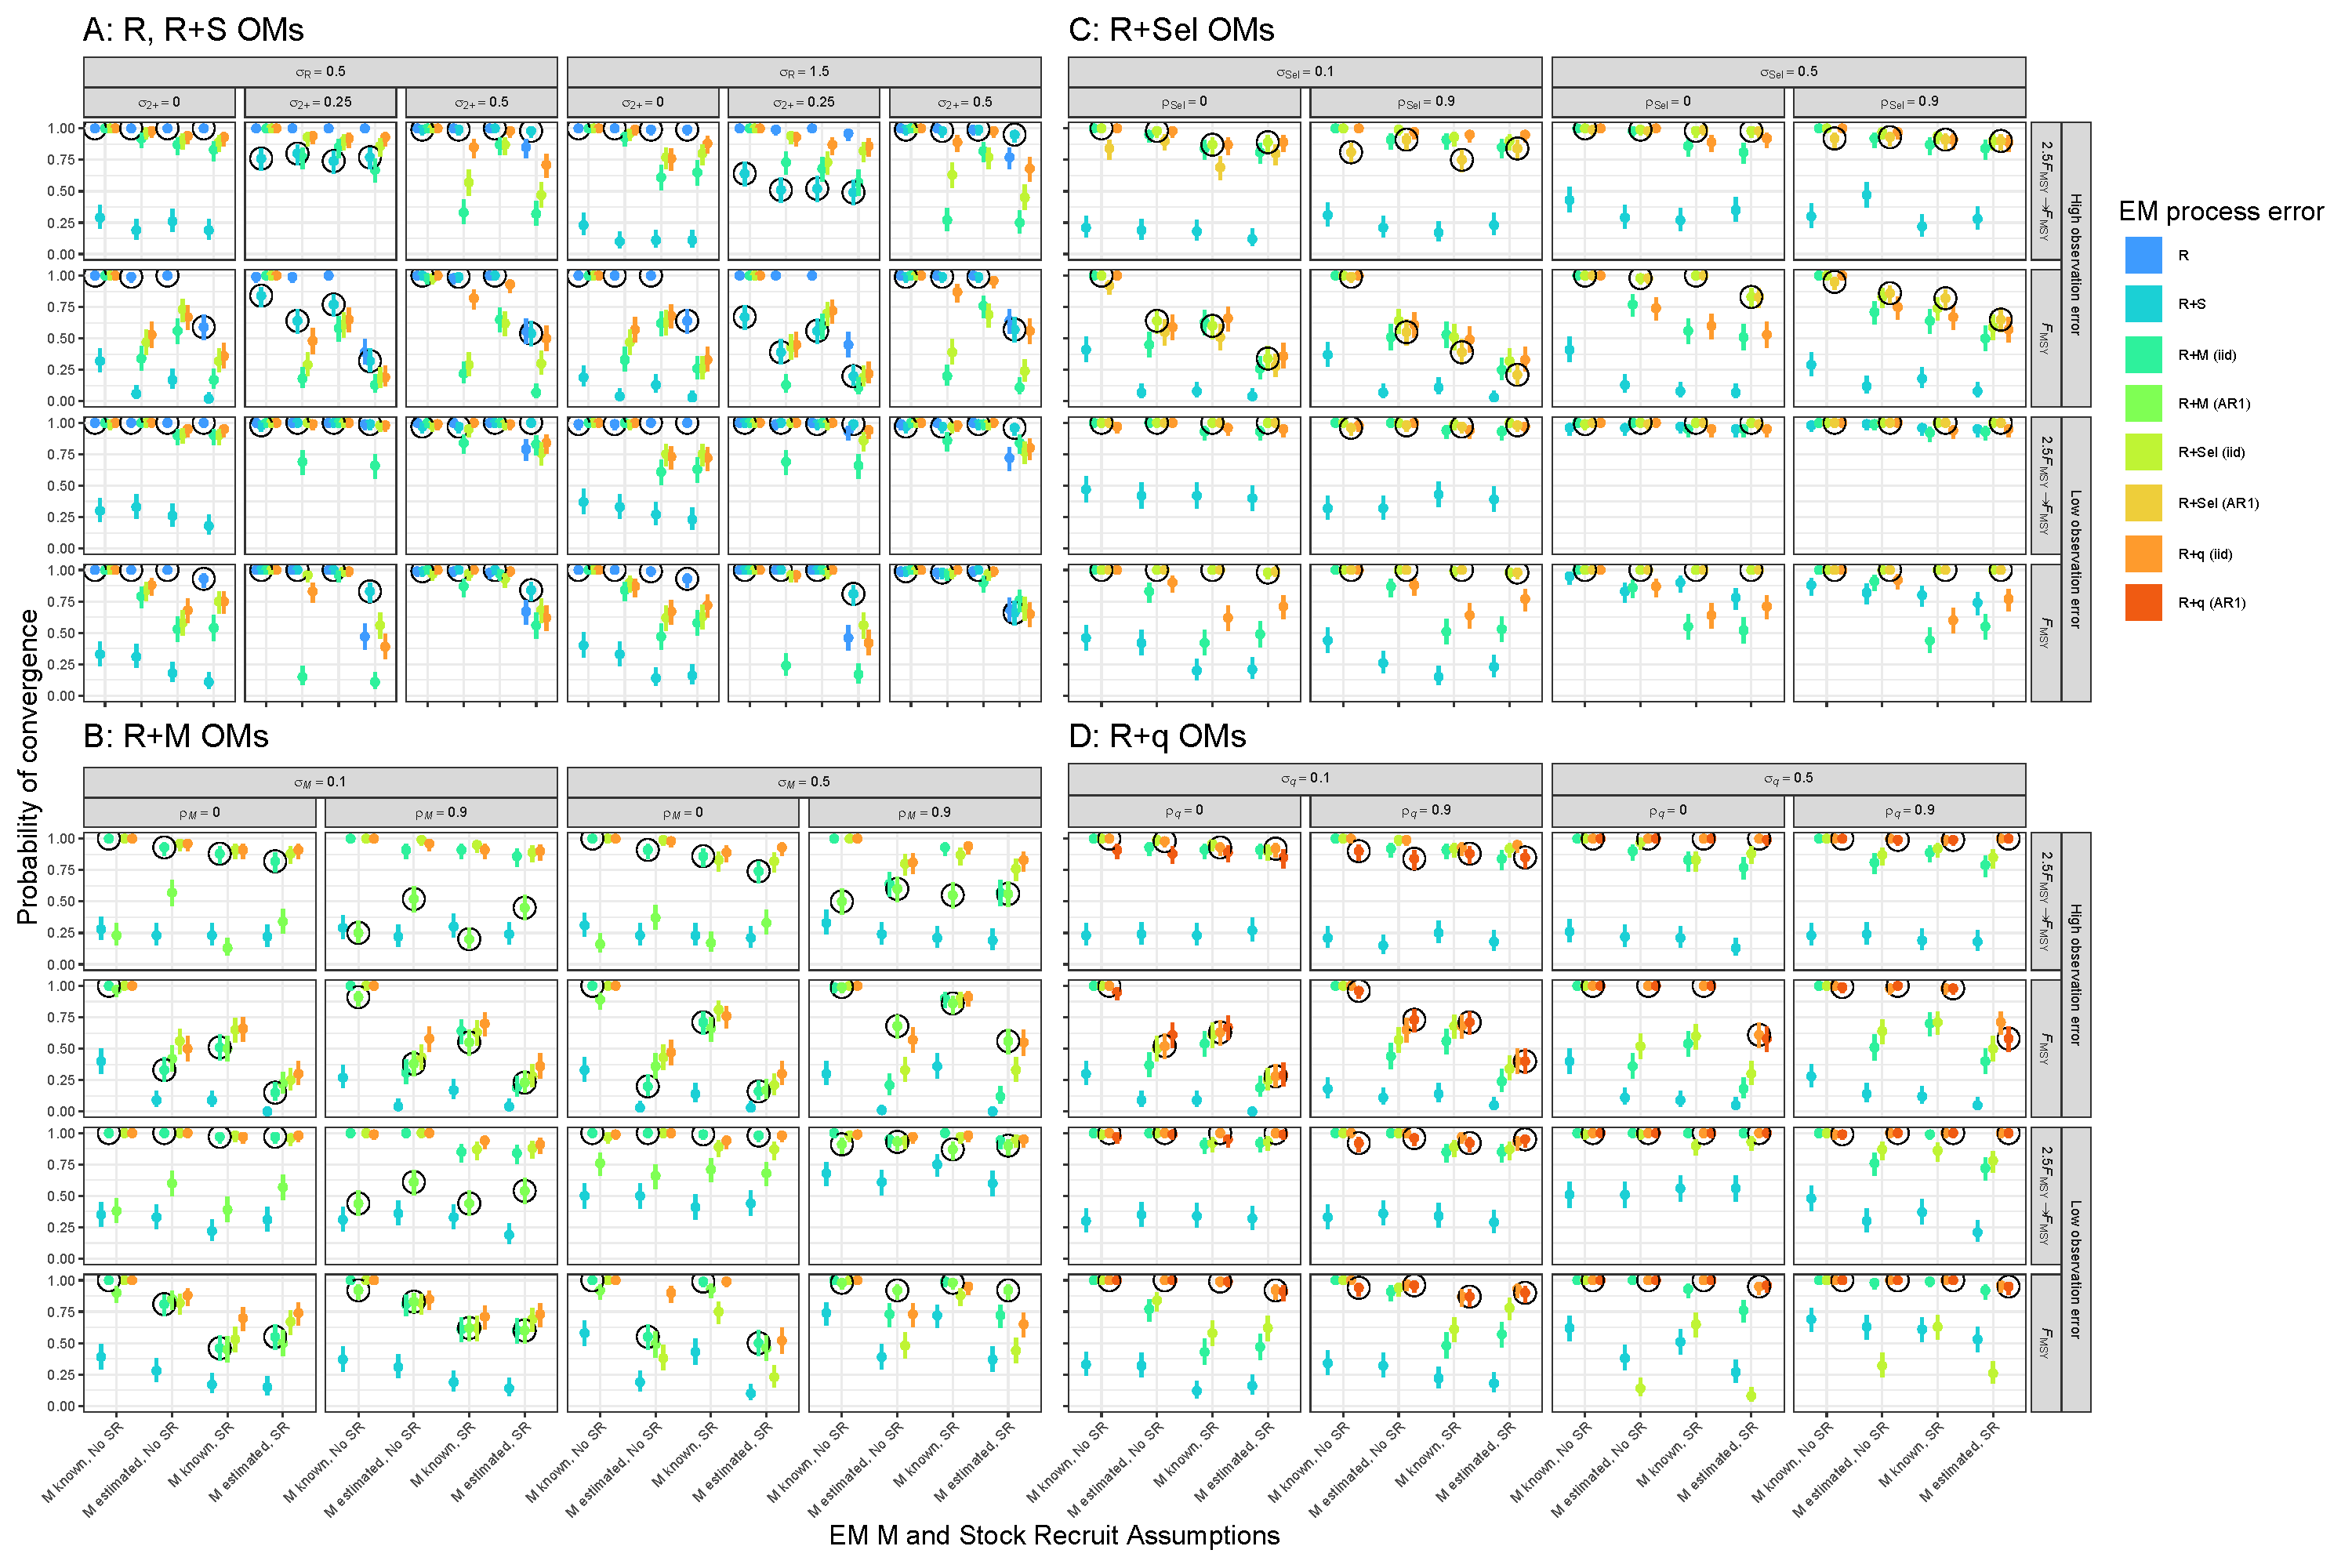
\includegraphics{type_4_convergence_plots}
\end{center}
\caption{Estimated probability of fits providing hessian-based standard errors for EMs assuming alternative process error (colored points and lines), and median natural mortality (estimated or known) and Beverton-Holt stock recruit functions (estimated or not; along x-axis) when fitted to operating models that have R and R+S (A), R+Sel (B), R+M (C), or R+q (D) process error structures. Circled values indicate results where the EM process error structure matches that of the operating model and vertical lines represent 95\% confidence intervals.}\label{hessian_SE_convergence}
\end{figure}
\end{landscape}

\clearpage

\begin{landscape}
\begin{figure}
\begin{center}
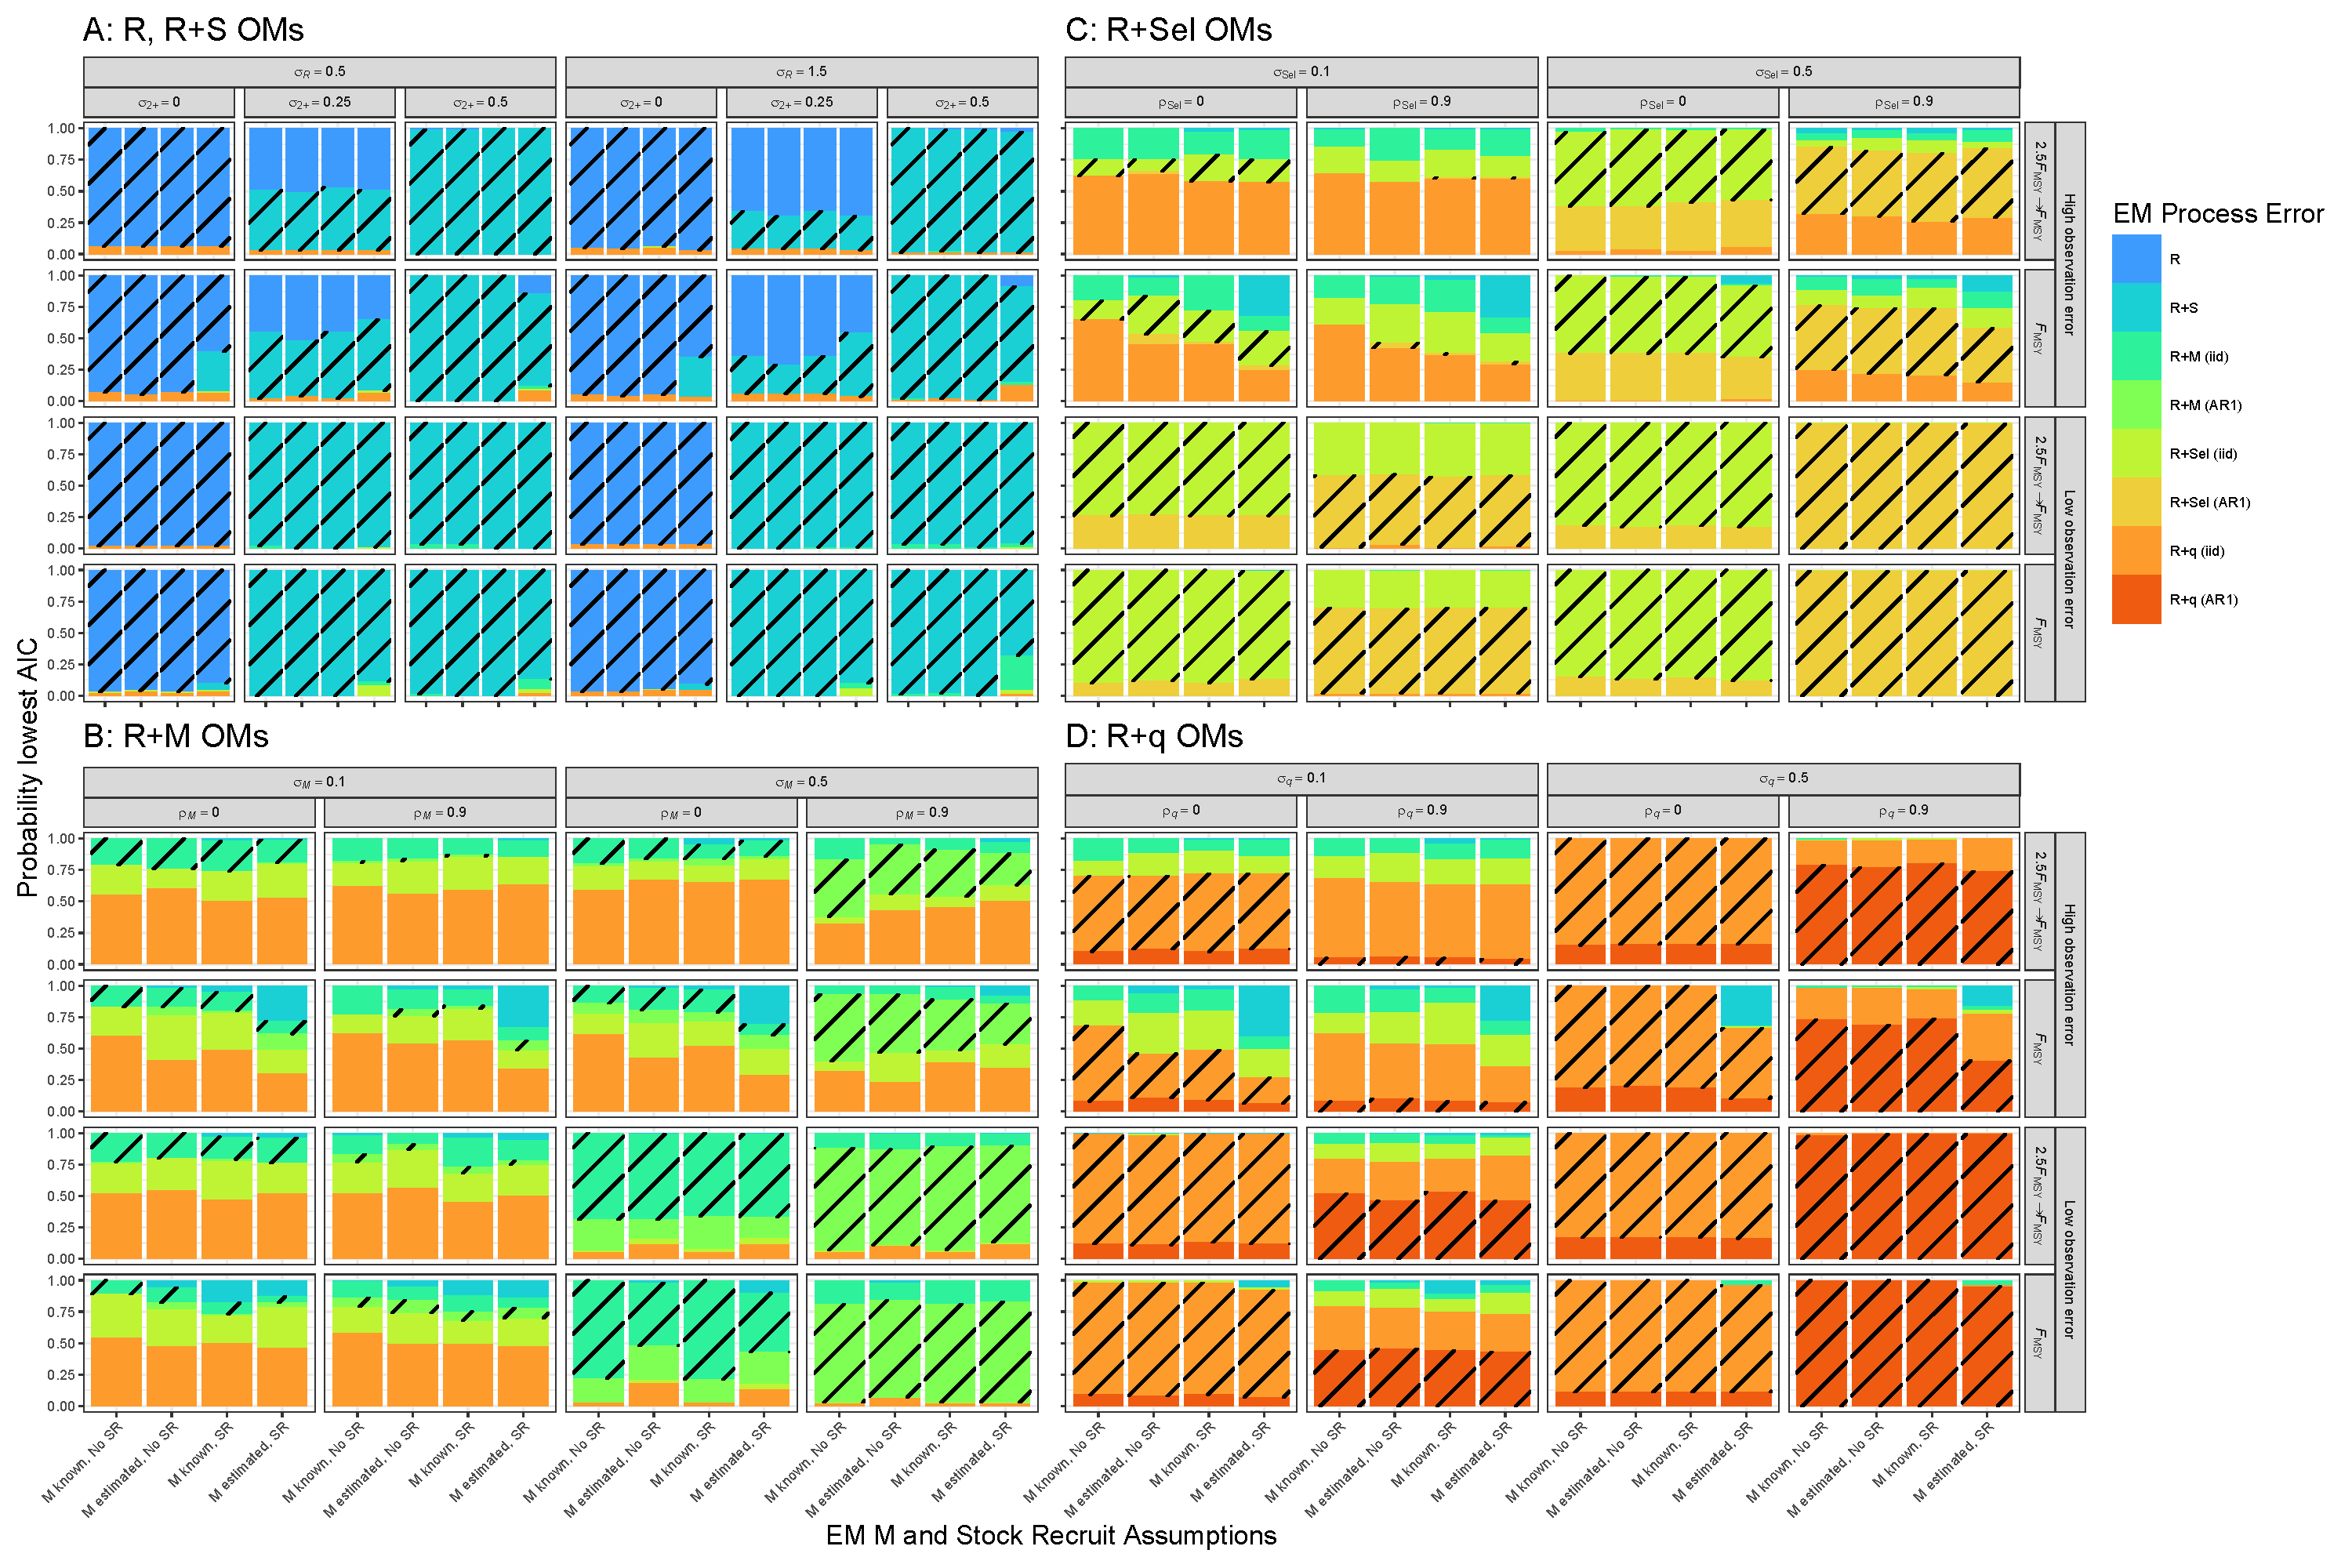
\includegraphics{pe_aic_plots}
\end{center}
\caption{Estimated probability of lowest AIC for EMs assuming alternative process error structures (colored bars) conditional on alternative assumptions for median natural mortality (estimated or known) and Beverton-Holt stock recruit functions (estimated or not; along x-axis) when fitted to operating models that have R and R+S (A), R+Sel (B), R+M (C), or R+q (D) process error structures. Striped bars indicate results where the EM process error structure matches that of the operating model.}\label{pe_aic}
\end{figure}
\end{landscape}

\clearpage

\begin{landscape}
\begin{figure}
\begin{center}
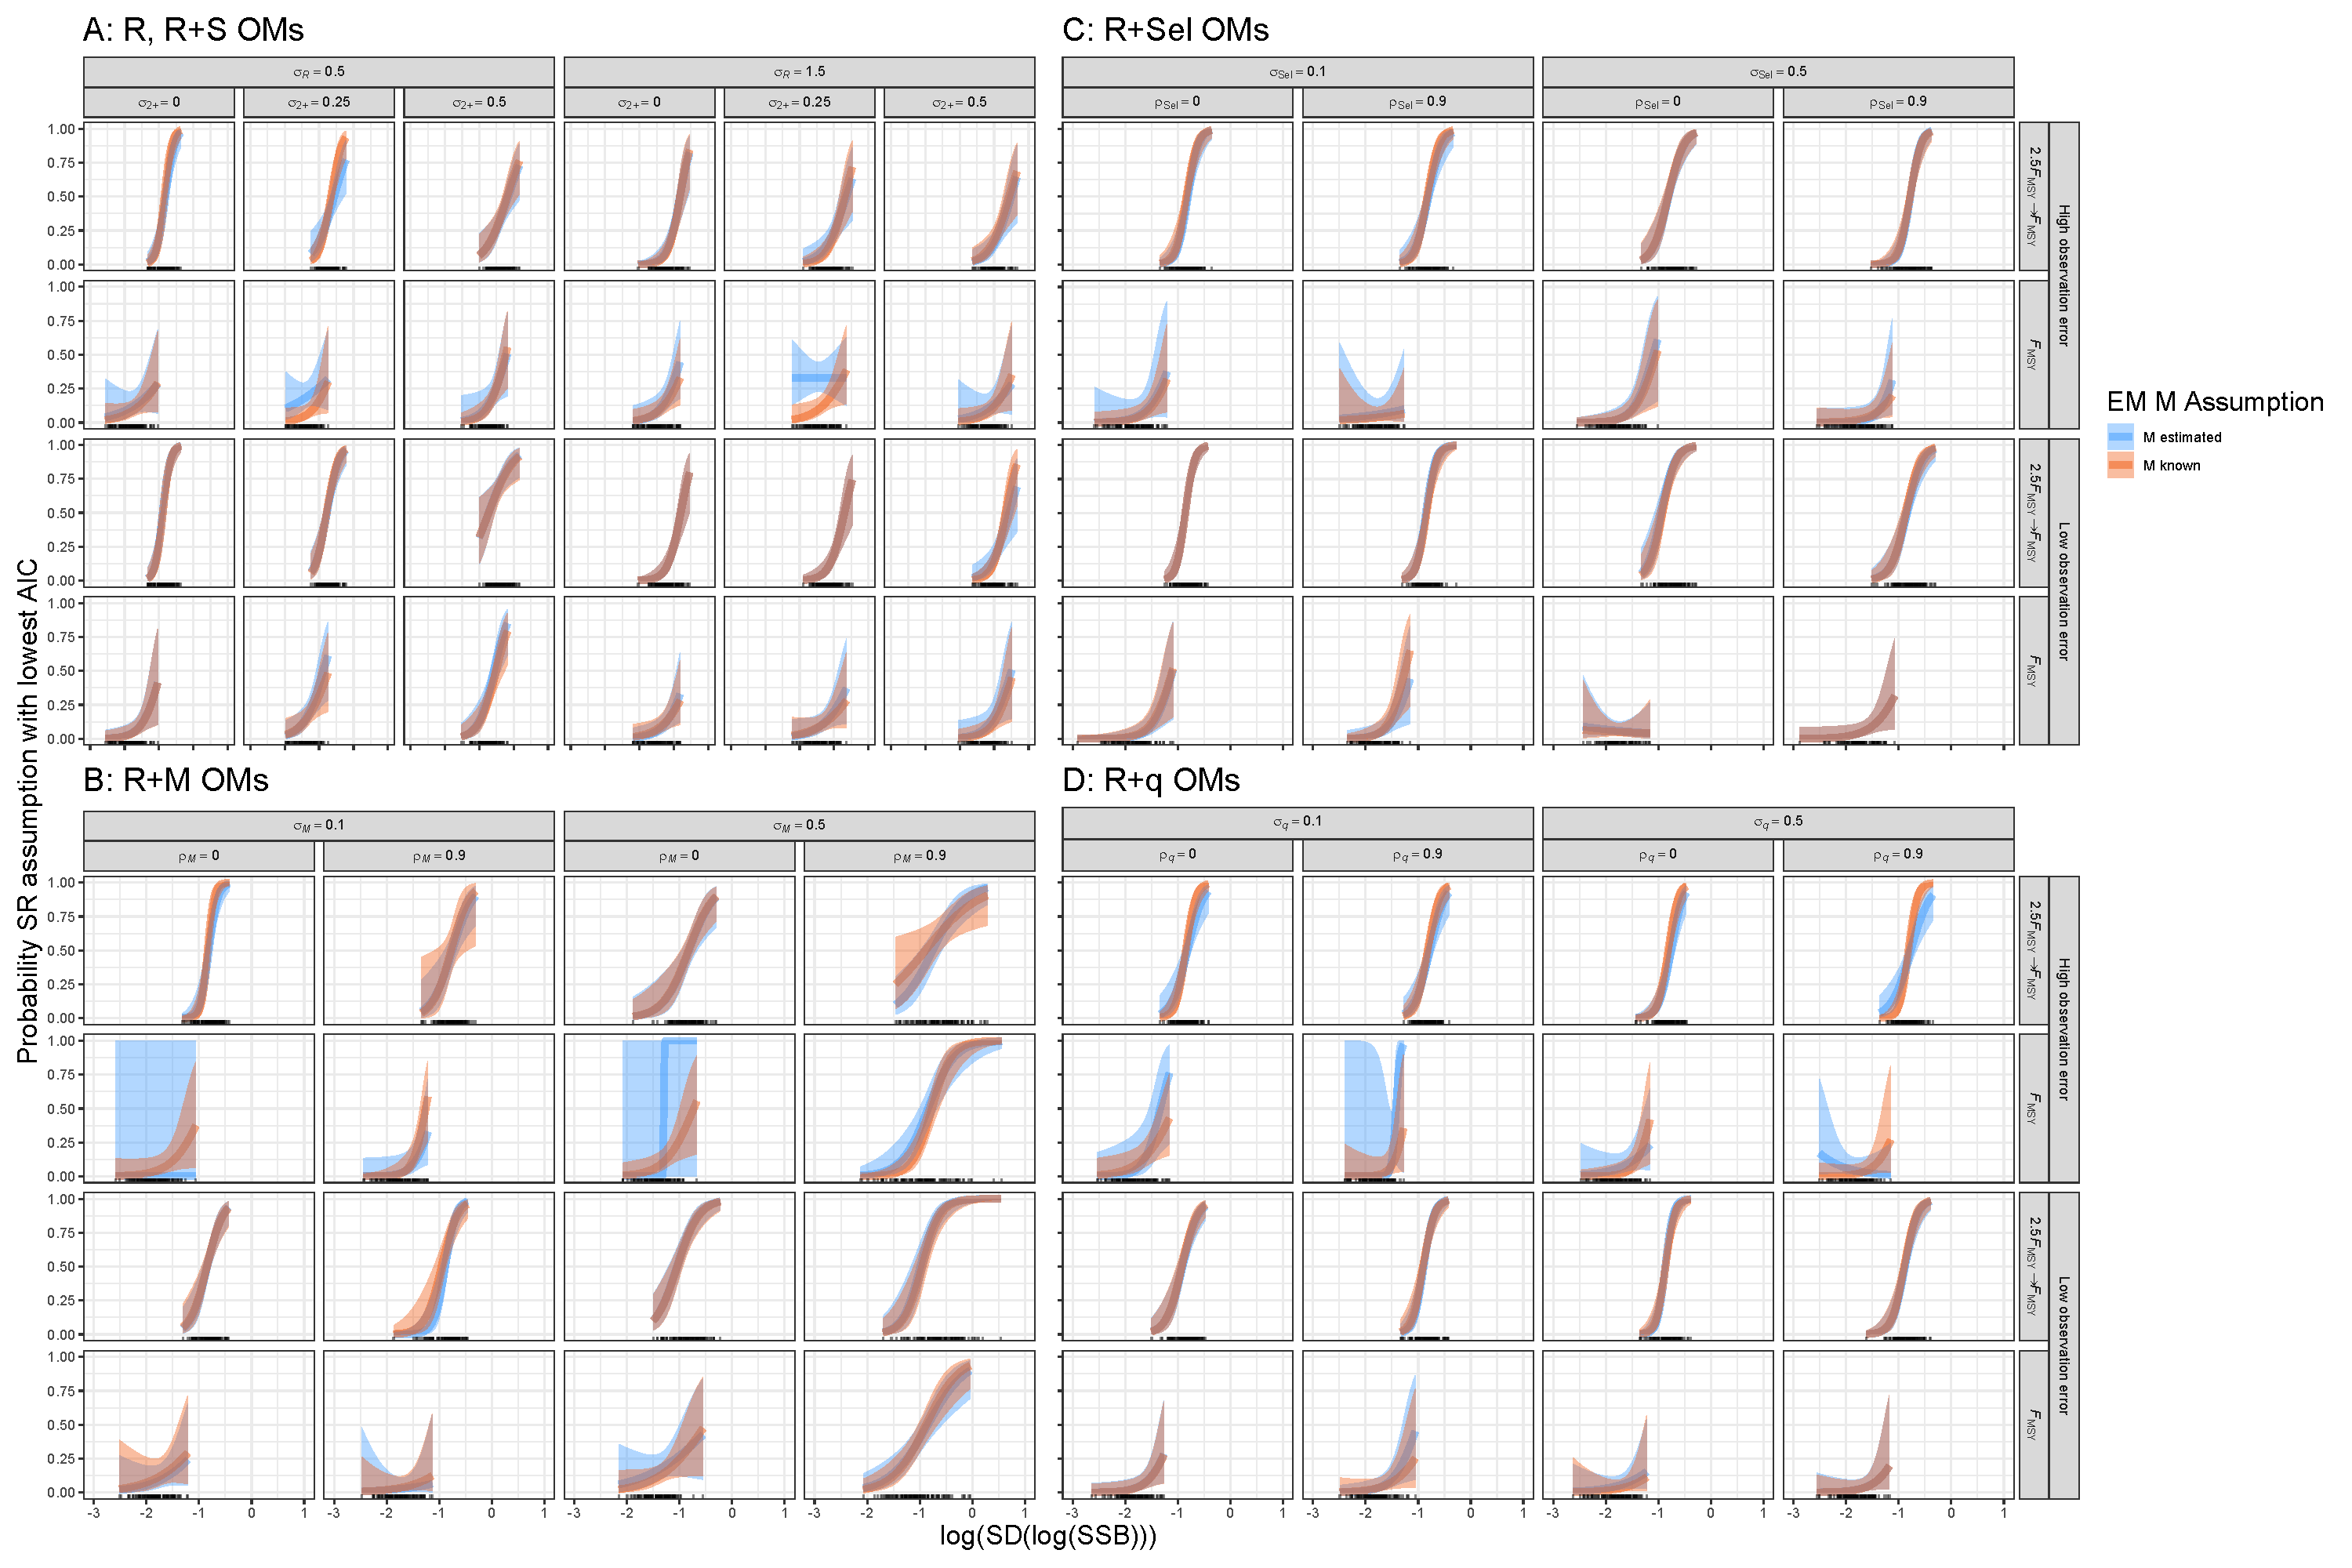
\includegraphics{sr_aic_plots}
\end{center}
\caption{Estimated probability of lowest AIC from logistic regression on the log-standard deviation of the true log(SSB) in each simulation for estimating model with Beverton-Holt stock recruit functions, rather than the otherwise equivalent EM without the stock recruit function. Results are conditional on alternative assumptions for median natural mortality (estimated or known) and on EMs having the correct process error structure: R and R+S (A), R+Sel (B), R+M (C), or R+q (D). Rug along x-axis denotes $SD(\log(SSB))$ values for each simulation amd polygons represent 95\% confidence intervals.}\label{sr_aic}
\end{figure}
\end{landscape}

\begin{landscape}
\begin{figure}
\begin{center}
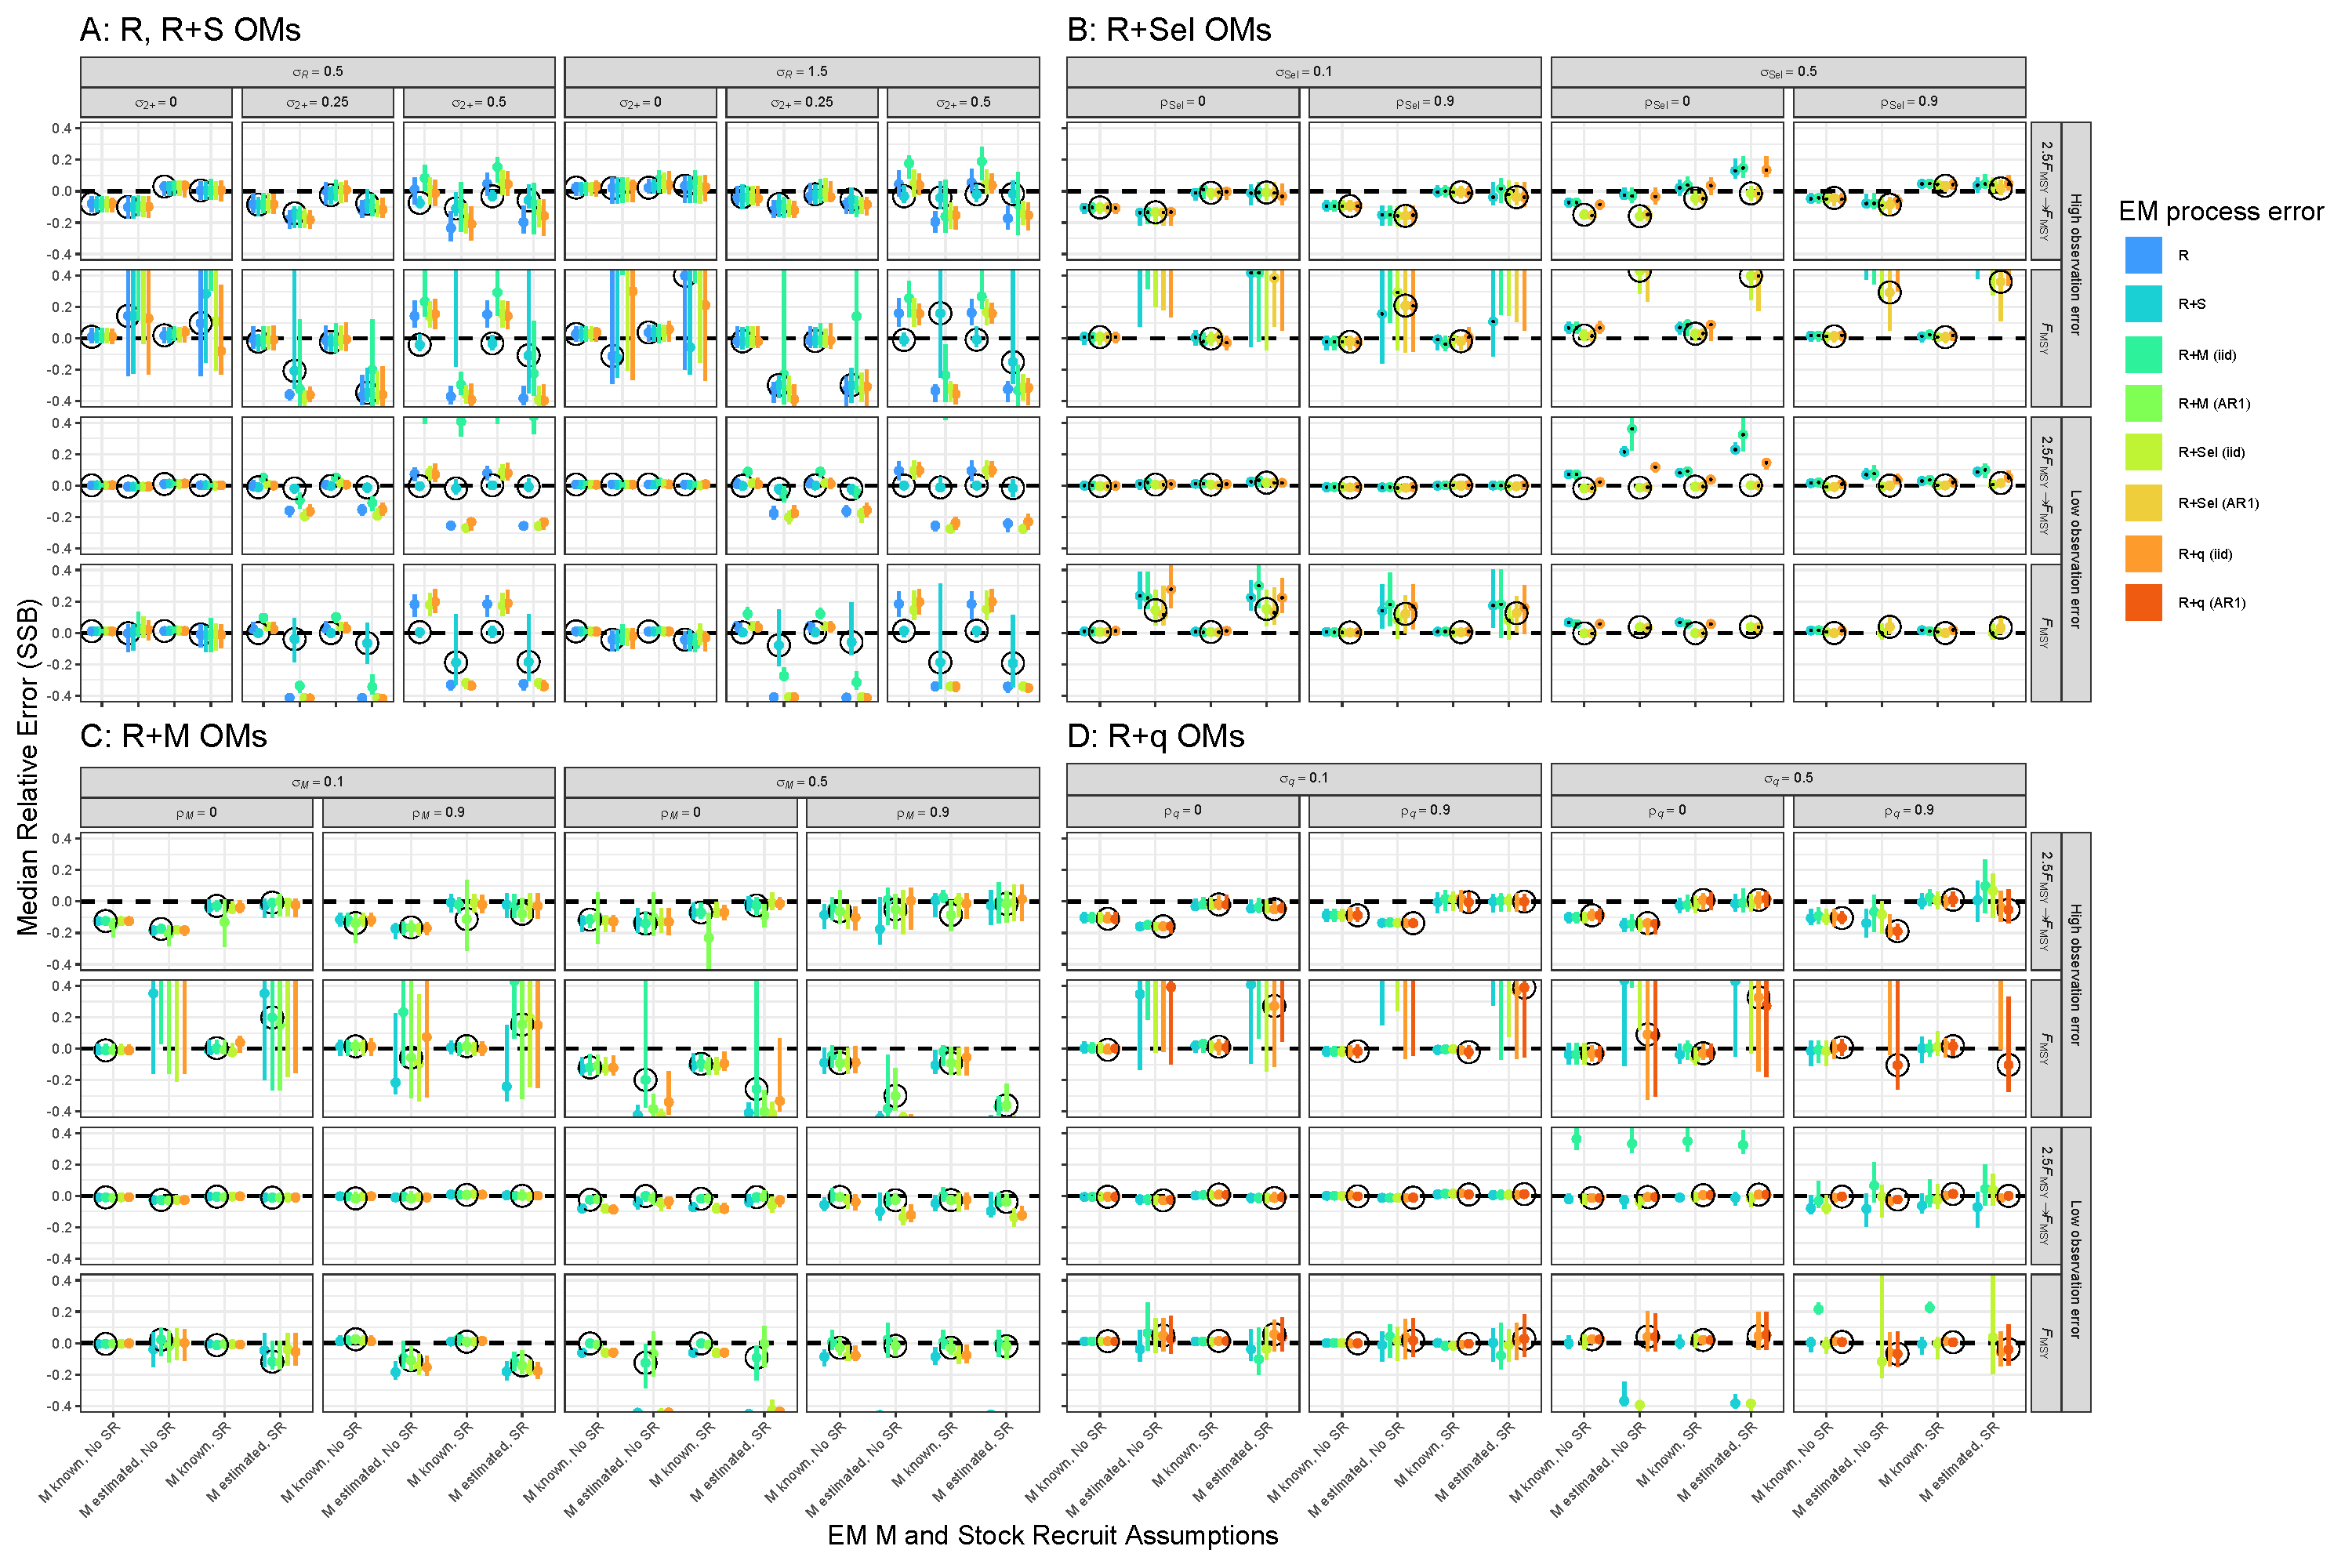
\includegraphics{term_SSB_bias_plots}
\end{center}
\caption{Median relative error of terminal year SSB for estimating models fitted to data sets simulated with alternative process error structures: R and R+S (A), R+Sel (B), R+M (C), or R+q (D).  Diamond shaped points denote results where the EM process error assumption matches that of the operating model. Circled values indicate results where the EM process error structure matches that of the operating model and vertical lines represent 95\% confidence intervals.}\label{SSB_rel_error}
\end{figure}
\end{landscape}

\begin{landscape}
\begin{figure}
\begin{center}
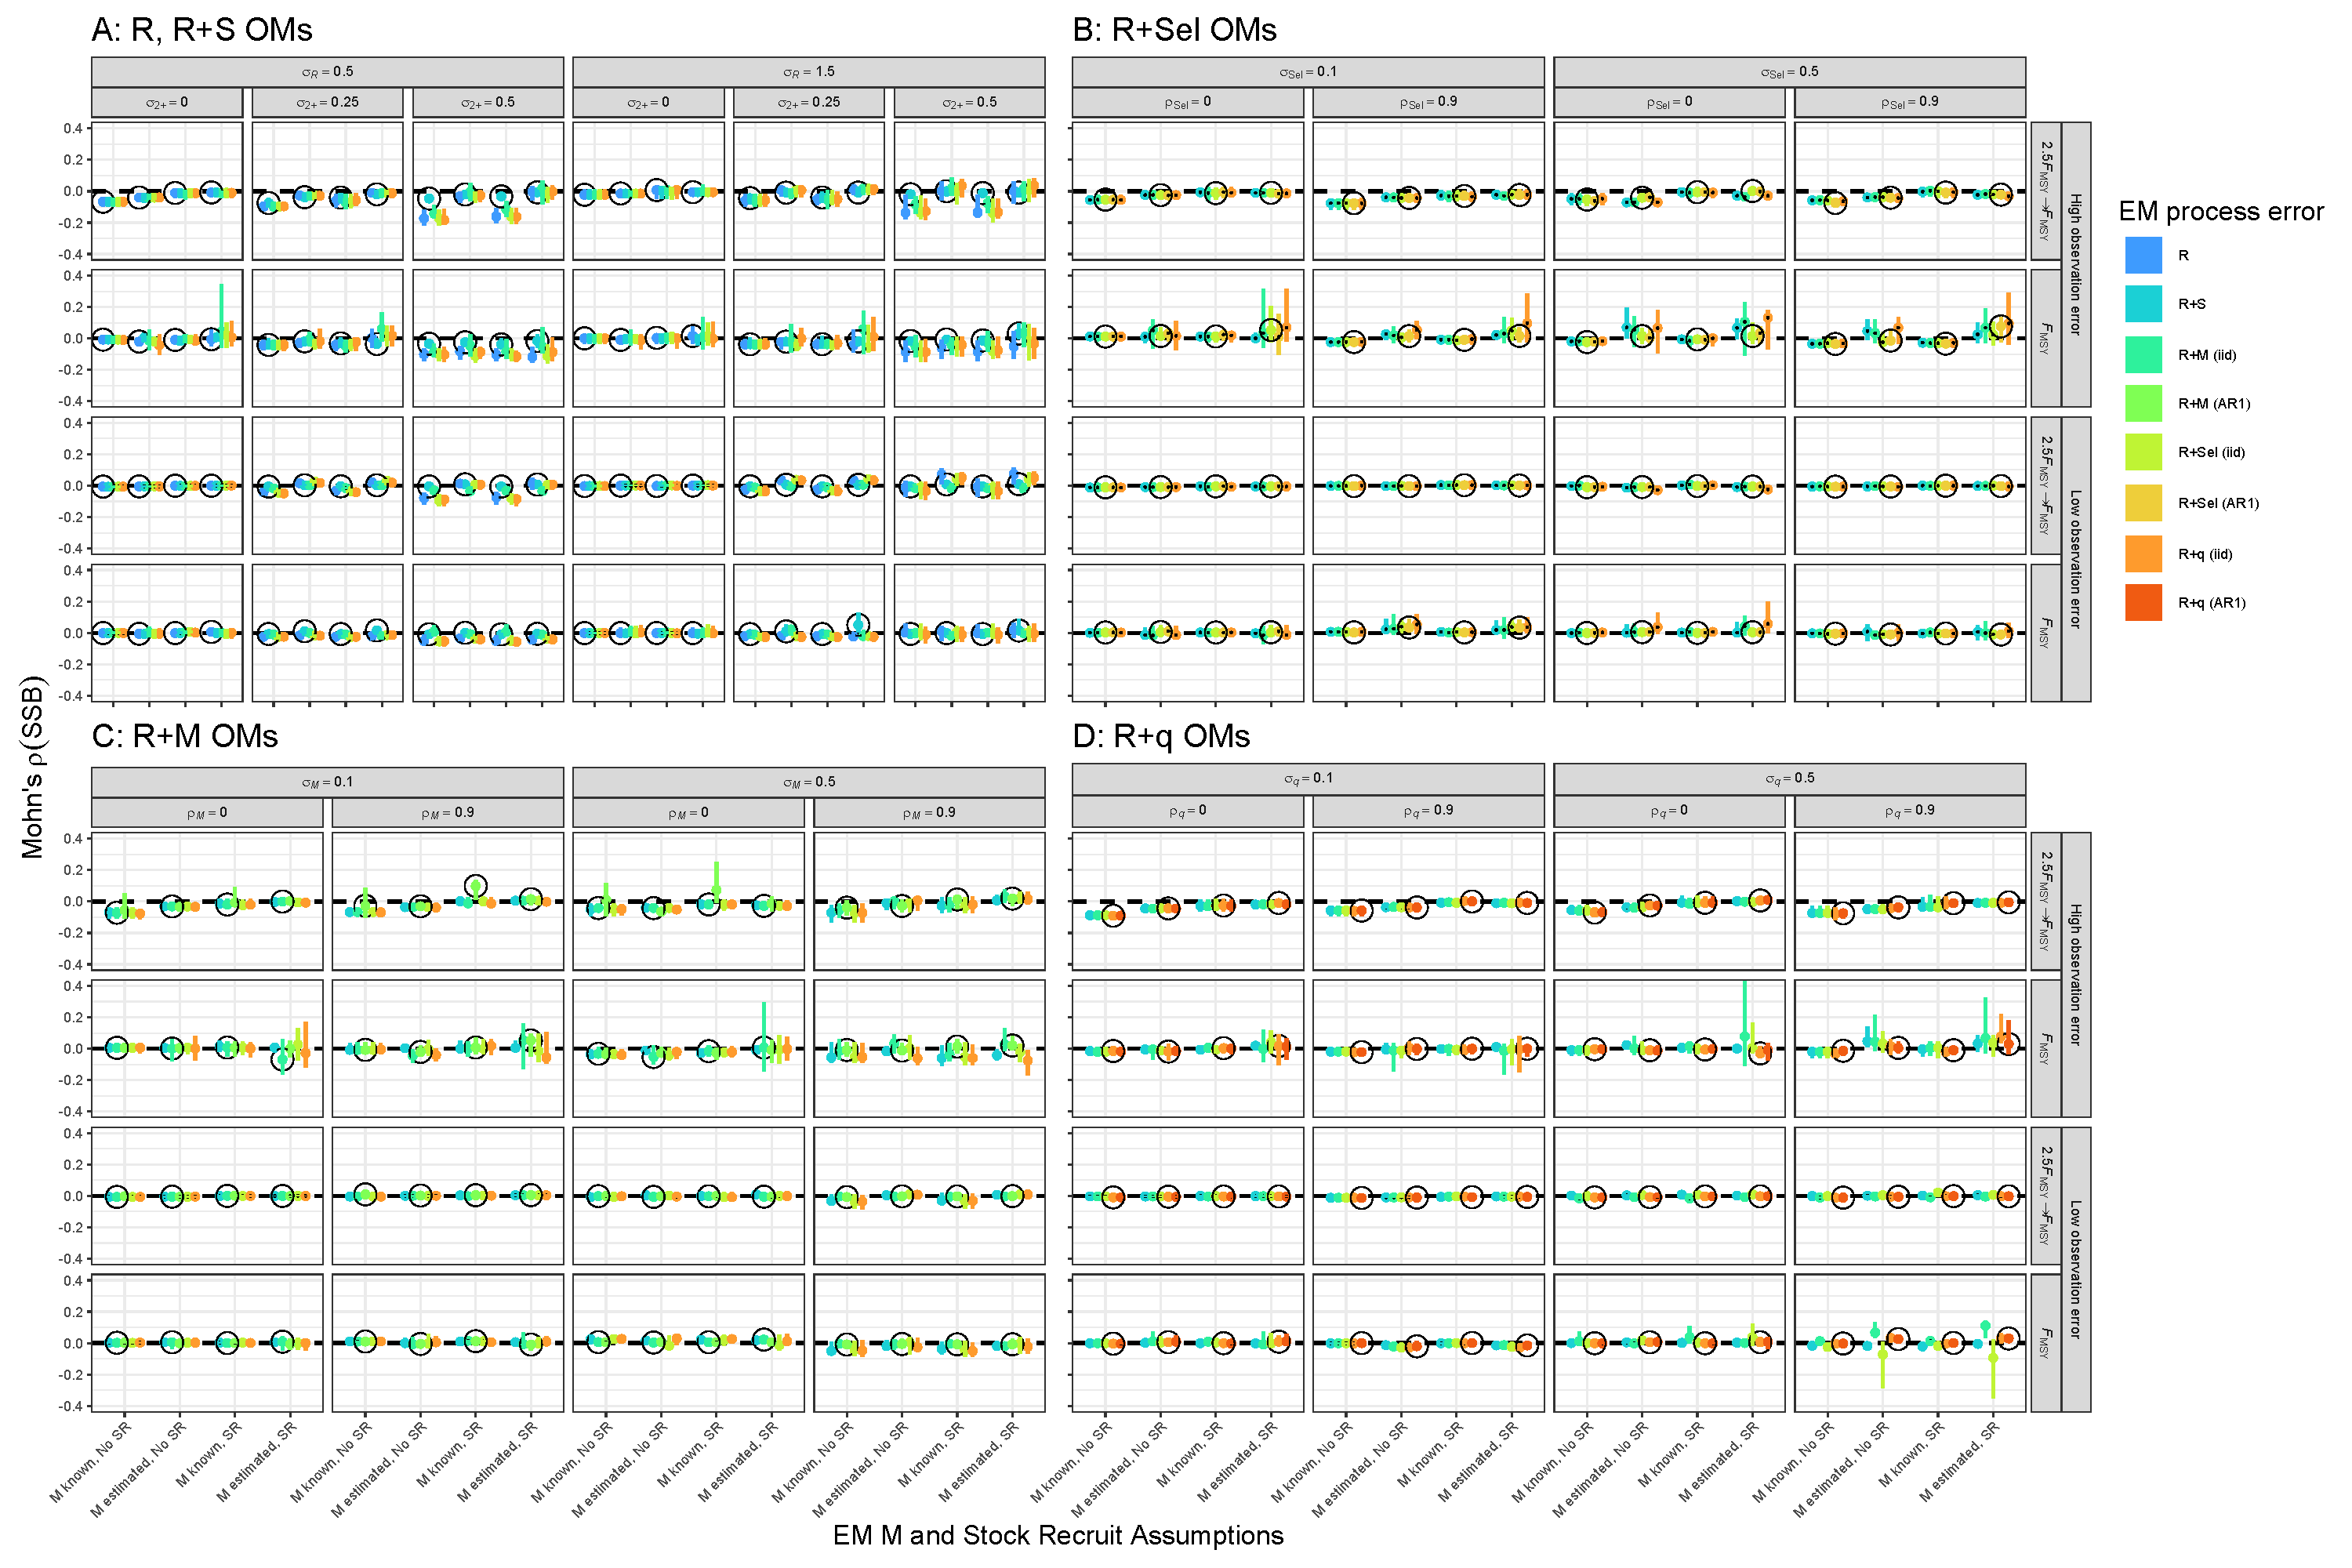
\includegraphics{mohns_rho_ssb_plots}
\end{center}
\caption{Median Mohn's rho for SSB for estimating models fitted to data sets simulated with alternative process error structures: R and R+S (A), R+Sel (B), R+M (C), or R+q (D). Circled values indicate results where the EM process error structure matches that of the operating model and vertical lines represent 95\% confidence intervals.}\label{mohns_rho_ssb}
\end{figure}
\end{landscape}

\pagebreak

\setcounter{figure}{0}
\renewcommand\thefigure{S\arabic{figure}}

\setcounter{table}{0}
\renewcommand\thetable{S\arabic{table}}

\hypertarget{supplementary-materials}{%
\section*{Supplementary Materials}\label{supplementary-materials}}
\addcontentsline{toc}{section}{Supplementary Materials}

\begin{figure}[!ht]
\begin{center}
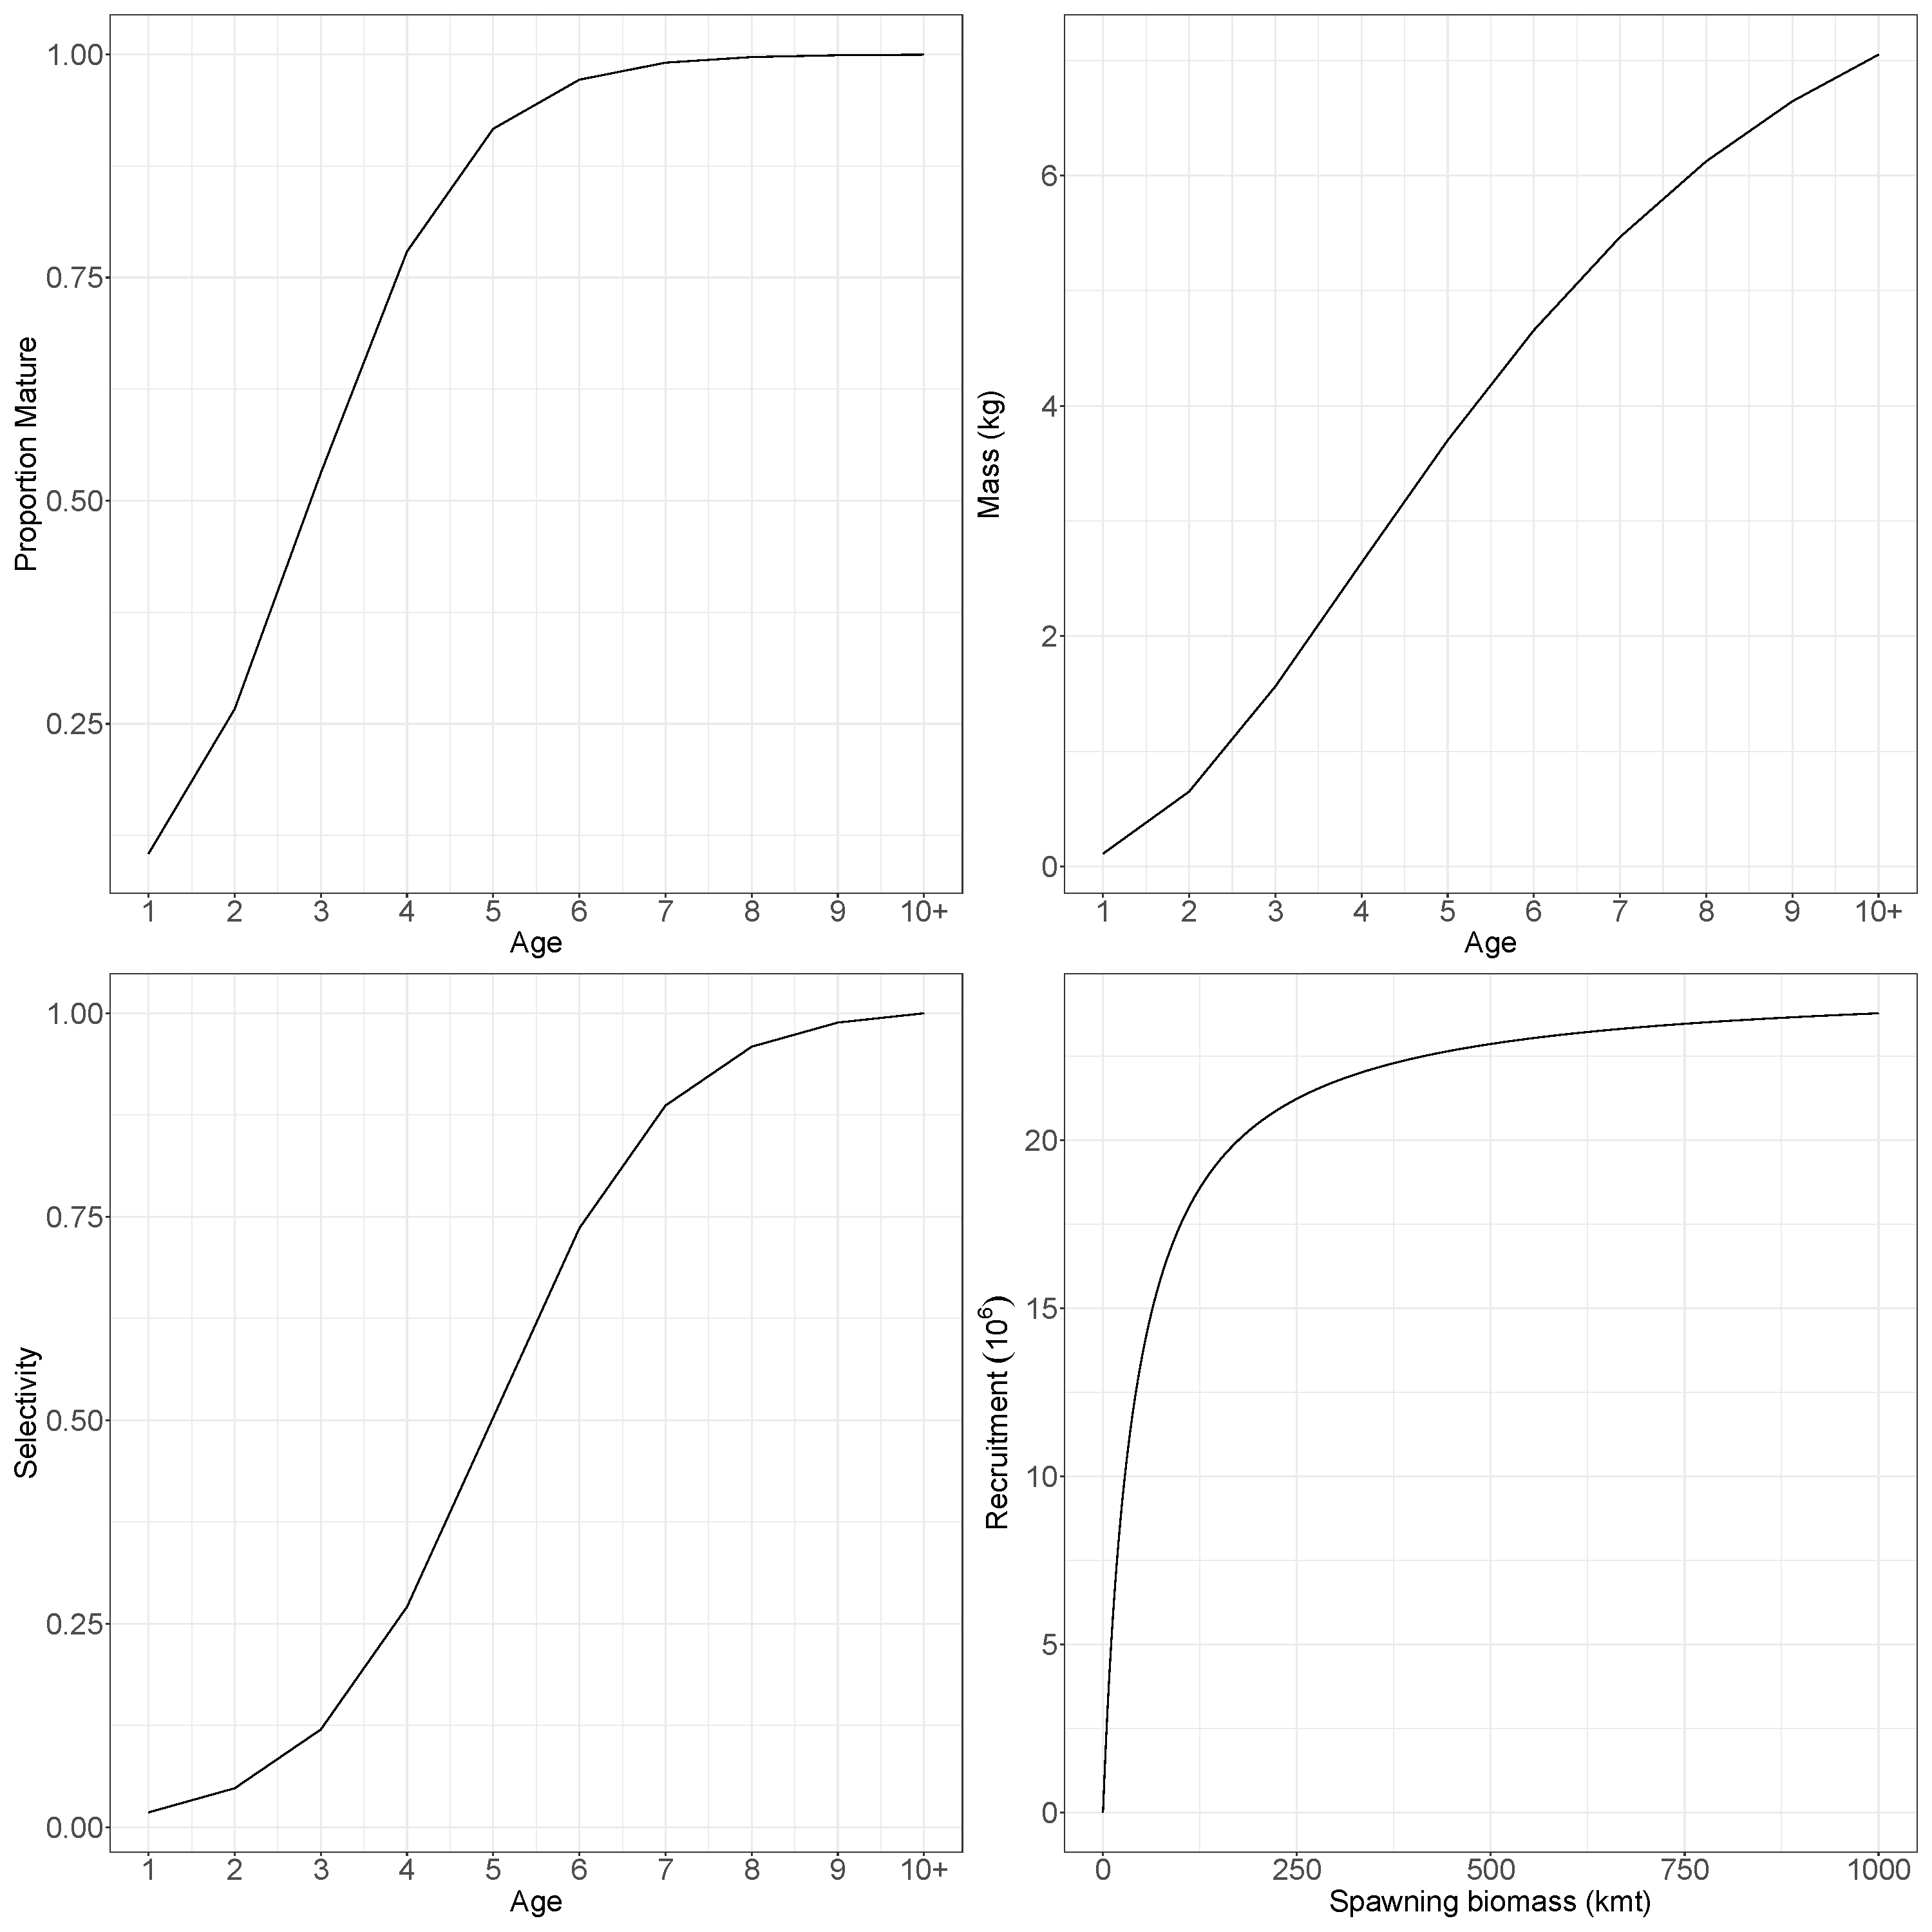
\includegraphics[width = \textwidth]{om_input_plots_figure}
\end{center}
\caption{The proportion mature at age, weight at age, fleet and index selectivity at age, and Beverton-Holt stock recruit relationship assumed for the population in all operating models. For operating models with random effects on fleet selectivity, this represents the selectivity at the mean of the random effects.}\label{om_inputs_fig}
\end{figure}

\begin{landscape}
\begin{table}
\caption{Distinguishing characteristics of the operating models with random effects on survival. Standard deviations (SD) are for log-normal distributed indices and logistic normal distributed age composition observations (fleet and indices). Fishing mortality changes after year 20 (of 40) for fishing histories where fishing mortality is not constant.}\label{naa_om_table}
{\footnotesize \begin{center}
\begin{tabular}{rrrrr}
\hline\hline
\multicolumn{1}{c}{Model}&\multicolumn{1}{c}{$\sigma_R$}&\multicolumn{1}{c}{$\sigma_{2+}$}&\multicolumn{1}{c}{Fishing History}&\multicolumn{1}{c}{Observation Uncertainty}\tabularnewline
\hline
NAA_1&$0.5$&$$&$2.5 F_{\text{MSY}} \rightarrow F_{\text{MSY}}$&Index sigma (log scale) = 0.1, Age composition sigma (logistic normal) = 0.3\tabularnewline
NAA_2&$1.5$&$$&$2.5 F_{\text{MSY}} \rightarrow F_{\text{MSY}}$&Index sigma (log scale) = 0.1, Age composition sigma (logistic normal) = 0.3\tabularnewline
NAA_3&$0.5$&$0.25$&$2.5 F_{\text{MSY}} \rightarrow F_{\text{MSY}}$&Index sigma (log scale) = 0.1, Age composition sigma (logistic normal) = 0.3\tabularnewline
NAA_4&$1.5$&$0.25$&$2.5 F_{\text{MSY}} \rightarrow F_{\text{MSY}}$&Index sigma (log scale) = 0.1, Age composition sigma (logistic normal) = 0.3\tabularnewline
NAA_5&$0.5$&$0.50$&$2.5 F_{\text{MSY}} \rightarrow F_{\text{MSY}}$&Index sigma (log scale) = 0.1, Age composition sigma (logistic normal) = 0.3\tabularnewline
NAA_6&$1.5$&$0.50$&$2.5 F_{\text{MSY}} \rightarrow F_{\text{MSY}}$&Index sigma (log scale) = 0.1, Age composition sigma (logistic normal) = 0.3\tabularnewline
NAA_7&$0.5$&$$&F_{\text{MSY}}&Index sigma (log scale) = 0.1, Age composition sigma (logistic normal) = 0.3\tabularnewline
NAA_8&$1.5$&$$&F_{\text{MSY}}&Index sigma (log scale) = 0.1, Age composition sigma (logistic normal) = 0.3\tabularnewline
NAA_9&$0.5$&$0.25$&F_{\text{MSY}}&Index sigma (log scale) = 0.1, Age composition sigma (logistic normal) = 0.3\tabularnewline
NAA_10&$1.5$&$0.25$&F_{\text{MSY}}&Index sigma (log scale) = 0.1, Age composition sigma (logistic normal) = 0.3\tabularnewline
NAA_11&$0.5$&$0.50$&F_{\text{MSY}}&Index sigma (log scale) = 0.1, Age composition sigma (logistic normal) = 0.3\tabularnewline
NAA_12&$1.5$&$0.50$&F_{\text{MSY}}&Index sigma (log scale) = 0.1, Age composition sigma (logistic normal) = 0.3\tabularnewline
NAA_13&$0.5$&$$&$2.5 F_{\text{MSY}} \rightarrow F_{\text{MSY}}$&Index sigma (log scale) = 0.4, Age composition sigma (logistic normal) = 1.5\tabularnewline
NAA_14&$1.5$&$$&$2.5 F_{\text{MSY}} \rightarrow F_{\text{MSY}}$&Index sigma (log scale) = 0.4, Age composition sigma (logistic normal) = 1.5\tabularnewline
NAA_15&$0.5$&$0.25$&$2.5 F_{\text{MSY}} \rightarrow F_{\text{MSY}}$&Index sigma (log scale) = 0.4, Age composition sigma (logistic normal) = 1.5\tabularnewline
NAA_16&$1.5$&$0.25$&$2.5 F_{\text{MSY}} \rightarrow F_{\text{MSY}}$&Index sigma (log scale) = 0.4, Age composition sigma (logistic normal) = 1.5\tabularnewline
NAA_17&$0.5$&$0.50$&$2.5 F_{\text{MSY}} \rightarrow F_{\text{MSY}}$&Index sigma (log scale) = 0.4, Age composition sigma (logistic normal) = 1.5\tabularnewline
NAA_18&$1.5$&$0.50$&$2.5 F_{\text{MSY}} \rightarrow F_{\text{MSY}}$&Index sigma (log scale) = 0.4, Age composition sigma (logistic normal) = 1.5\tabularnewline
NAA_19&$0.5$&$$&F_{\text{MSY}}&Index sigma (log scale) = 0.4, Age composition sigma (logistic normal) = 1.5\tabularnewline
NAA_20&$1.5$&$$&F_{\text{MSY}}&Index sigma (log scale) = 0.4, Age composition sigma (logistic normal) = 1.5\tabularnewline
NAA_21&$0.5$&$0.25$&F_{\text{MSY}}&Index sigma (log scale) = 0.4, Age composition sigma (logistic normal) = 1.5\tabularnewline
NAA_22&$1.5$&$0.25$&F_{\text{MSY}}&Index sigma (log scale) = 0.4, Age composition sigma (logistic normal) = 1.5\tabularnewline
NAA_23&$0.5$&$0.50$&F_{\text{MSY}}&Index sigma (log scale) = 0.4, Age composition sigma (logistic normal) = 1.5\tabularnewline
NAA_24&$1.5$&$0.50$&F_{\text{MSY}}&Index sigma (log scale) = 0.4, Age composition sigma (logistic normal) = 1.5\tabularnewline
\hline
\end{tabular}\end{center}
}
\end{table}
\end{landscape}

\begin{landscape}
\begin{table}
\caption{Distinguishing characteristics of the operating models with random effects on natural mortality. Standard deviations (SD) are for log-normal distributed indices and logistic normal distributed age composition observations (fleet and indices). Fishing mortality changes after year 20 (of 40) for fishing histories where fishing mortality is not constant. For AR1 process errors, $\sigma$ is defined for the marginal distribution of the processes.}\label{M_om_table}
{\begin{center}
\begin{tabular}{rrrrrr}
\hline\hline
\multicolumn{1}{c}{Model}&\multicolumn{1}{c}{$\sigma_R$}&\multicolumn{1}{c}{$\sigma_{M}$}&\multicolumn{1}{c}{$\rho_{M}$}&\multicolumn{1}{c}{Fishing History}&\multicolumn{1}{c}{Observation Uncertainty}\tabularnewline
\hline
$M_{1}$&$0.5$&$0.1$&$0.0$&$2.5 F_{\text{MSY}} \rightarrow F_{\text{MSY}}$&Index SD = 0.1, Age composition SD = 0.3\tabularnewline
$M_{2}$&$0.5$&$0.5$&$0.0$&$2.5 F_{\text{MSY}} \rightarrow F_{\text{MSY}}$&Index SD = 0.1, Age composition SD = 0.3\tabularnewline
$M_{3}$&$0.5$&$0.1$&$0.9$&$2.5 F_{\text{MSY}} \rightarrow F_{\text{MSY}}$&Index SD = 0.1, Age composition SD = 0.3\tabularnewline
$M_{4}$&$0.5$&$0.5$&$0.9$&$2.5 F_{\text{MSY}} \rightarrow F_{\text{MSY}}$&Index SD = 0.1, Age composition SD = 0.3\tabularnewline
$M_{5}$&$0.5$&$0.1$&$0.0$&$F_{\text{MSY}}$&Index SD = 0.1, Age composition SD = 0.3\tabularnewline
$M_{6}$&$0.5$&$0.5$&$0.0$&$F_{\text{MSY}}$&Index SD = 0.1, Age composition SD = 0.3\tabularnewline
$M_{7}$&$0.5$&$0.1$&$0.9$&$F_{\text{MSY}}$&Index SD = 0.1, Age composition SD = 0.3\tabularnewline
$M_{8}$&$0.5$&$0.5$&$0.9$&$F_{\text{MSY}}$&Index SD = 0.1, Age composition SD = 0.3\tabularnewline
$M_{9}$&$0.5$&$0.1$&$0.0$&$2.5 F_{\text{MSY}} \rightarrow F_{\text{MSY}}$&Index SD = 0.4, Age composition SD = 1.5\tabularnewline
$M_{10}$&$0.5$&$0.5$&$0.0$&$2.5 F_{\text{MSY}} \rightarrow F_{\text{MSY}}$&Index SD = 0.4, Age composition SD = 1.5\tabularnewline
$M_{11}$&$0.5$&$0.1$&$0.9$&$2.5 F_{\text{MSY}} \rightarrow F_{\text{MSY}}$&Index SD = 0.4, Age composition SD = 1.5\tabularnewline
$M_{12}$&$0.5$&$0.5$&$0.9$&$2.5 F_{\text{MSY}} \rightarrow F_{\text{MSY}}$&Index SD = 0.4, Age composition SD = 1.5\tabularnewline
$M_{13}$&$0.5$&$0.1$&$0.0$&$F_{\text{MSY}}$&Index SD = 0.4, Age composition SD = 1.5\tabularnewline
$M_{14}$&$0.5$&$0.5$&$0.0$&$F_{\text{MSY}}$&Index SD = 0.4, Age composition SD = 1.5\tabularnewline
$M_{15}$&$0.5$&$0.1$&$0.9$&$F_{\text{MSY}}$&Index SD = 0.4, Age composition SD = 1.5\tabularnewline
$M_{16}$&$0.5$&$0.5$&$0.9$&$F_{\text{MSY}}$&Index SD = 0.4, Age composition SD = 1.5\tabularnewline
\hline
\end{tabular}\end{center}
}
\end{table}
\end{landscape}

\begin{landscape}
\begin{table}
\caption{Distinguishing characteristics of the operating models with random effects on selectivity. Standard deviations (SD) are for log-normal distributed indices and logistic normal distributed age composition observations (fleet and indices). Fishing mortality changes after year 20 (of 40) for fishing histories where fishing mortality is not constant. For AR1 process errors, $\sigma$ is defined for the marginal distribution of the processes.}\label{sel_om_table}
{\begin{center}
\begin{tabular}{rrrrrr}
\hline\hline
\multicolumn{1}{c}{Model}&\multicolumn{1}{c}{$\sigma_R$}&\multicolumn{1}{c}{$\sigma_{\text{Sel}}$}&\multicolumn{1}{c}{$\rho_{\text{Sel}}$}&\multicolumn{1}{c}{Fishing History}&\multicolumn{1}{c}{Observation Uncertainty}\tabularnewline
\hline
$\text{Sel}_{1}$&$0.5$&$0.1$&$0.0$&$2.5 F_{\text{MSY}} \rightarrow F_{\text{MSY}}$&Index SD = 0.1, Age composition SD = 0.3\tabularnewline
$\text{Sel}_{2}$&$0.5$&$0.5$&$0.0$&$2.5 F_{\text{MSY}} \rightarrow F_{\text{MSY}}$&Index SD = 0.1, Age composition SD = 0.3\tabularnewline
$\text{Sel}_{3}$&$0.5$&$0.1$&$0.9$&$2.5 F_{\text{MSY}} \rightarrow F_{\text{MSY}}$&Index SD = 0.1, Age composition SD = 0.3\tabularnewline
$\text{Sel}_{4}$&$0.5$&$0.5$&$0.9$&$2.5 F_{\text{MSY}} \rightarrow F_{\text{MSY}}$&Index SD = 0.1, Age composition SD = 0.3\tabularnewline
$\text{Sel}_{5}$&$0.5$&$0.1$&$0.0$&$F_{\text{MSY}}$&Index SD = 0.1, Age composition SD = 0.3\tabularnewline
$\text{Sel}_{6}$&$0.5$&$0.5$&$0.0$&$F_{\text{MSY}}$&Index SD = 0.1, Age composition SD = 0.3\tabularnewline
$\text{Sel}_{7}$&$0.5$&$0.1$&$0.9$&$F_{\text{MSY}}$&Index SD = 0.1, Age composition SD = 0.3\tabularnewline
$\text{Sel}_{8}$&$0.5$&$0.5$&$0.9$&$F_{\text{MSY}}$&Index SD = 0.1, Age composition SD = 0.3\tabularnewline
$\text{Sel}_{9}$&$0.5$&$0.1$&$0.0$&$2.5 F_{\text{MSY}} \rightarrow F_{\text{MSY}}$&Index SD = 0.4, Age composition SD = 1.5\tabularnewline
$\text{Sel}_{10}$&$0.5$&$0.5$&$0.0$&$2.5 F_{\text{MSY}} \rightarrow F_{\text{MSY}}$&Index SD = 0.4, Age composition SD = 1.5\tabularnewline
$\text{Sel}_{11}$&$0.5$&$0.1$&$0.9$&$2.5 F_{\text{MSY}} \rightarrow F_{\text{MSY}}$&Index SD = 0.4, Age composition SD = 1.5\tabularnewline
$\text{Sel}_{12}$&$0.5$&$0.5$&$0.9$&$2.5 F_{\text{MSY}} \rightarrow F_{\text{MSY}}$&Index SD = 0.4, Age composition SD = 1.5\tabularnewline
$\text{Sel}_{13}$&$0.5$&$0.1$&$0.0$&$F_{\text{MSY}}$&Index SD = 0.4, Age composition SD = 1.5\tabularnewline
$\text{Sel}_{14}$&$0.5$&$0.5$&$0.0$&$F_{\text{MSY}}$&Index SD = 0.4, Age composition SD = 1.5\tabularnewline
$\text{Sel}_{15}$&$0.5$&$0.1$&$0.9$&$F_{\text{MSY}}$&Index SD = 0.4, Age composition SD = 1.5\tabularnewline
$\text{Sel}_{16}$&$0.5$&$0.5$&$0.9$&$F_{\text{MSY}}$&Index SD = 0.4, Age composition SD = 1.5\tabularnewline
\hline
\end{tabular}\end{center}
}
\end{table}
\end{landscape}

\begin{landscape}
\begin{table}
\caption{Distinguishing characteristics of the operating models with random effects on catchability. Standard deviations (SD) are for log-normal distributed indices and logistic normal distributed age composition observations (fleet and indices). Fishing mortality changes after year 20 (of 40) for fishing histories where fishing mortality is not constant. For AR1 process errors, $\sigma$ is defined for the marginal distribution of the processes.}\label{q_om_table}
{\begin{center}
\begin{tabular}{rrrrrr}
\hline\hline
\multicolumn{1}{c}{Model}&\multicolumn{1}{c}{$\sigma_R$}&\multicolumn{1}{c}{$\sigma_{q}$}&\multicolumn{1}{c}{$\rho_{q}$}&\multicolumn{1}{c}{Fishing History}&\multicolumn{1}{c}{Observation Uncertainty}\tabularnewline
\hline
$q_{1}$&$0.5$&$0.1$&$0.0$&$2.5 F_{\text{MSY}} \rightarrow F_{\text{MSY}}$&Index SD = 0.1, Age composition SD = 0.3\tabularnewline
$q_{2}$&$0.5$&$0.5$&$0.0$&$2.5 F_{\text{MSY}} \rightarrow F_{\text{MSY}}$&Index SD = 0.1, Age composition SD = 0.3\tabularnewline
$q_{3}$&$0.5$&$0.1$&$0.9$&$2.5 F_{\text{MSY}} \rightarrow F_{\text{MSY}}$&Index SD = 0.1, Age composition SD = 0.3\tabularnewline
$q_{4}$&$0.5$&$0.5$&$0.9$&$2.5 F_{\text{MSY}} \rightarrow F_{\text{MSY}}$&Index SD = 0.1, Age composition SD = 0.3\tabularnewline
$q_{5}$&$0.5$&$0.1$&$0.0$&$F_{\text{MSY}}$&Index SD = 0.1, Age composition SD = 0.3\tabularnewline
$q_{6}$&$0.5$&$0.5$&$0.0$&$F_{\text{MSY}}$&Index SD = 0.1, Age composition SD = 0.3\tabularnewline
$q_{7}$&$0.5$&$0.1$&$0.9$&$F_{\text{MSY}}$&Index SD = 0.1, Age composition SD = 0.3\tabularnewline
$q_{8}$&$0.5$&$0.5$&$0.9$&$F_{\text{MSY}}$&Index SD = 0.1, Age composition SD = 0.3\tabularnewline
$q_{9}$&$0.5$&$0.1$&$0.0$&$2.5 F_{\text{MSY}} \rightarrow F_{\text{MSY}}$&Index SD = 0.4, Age composition SD = 1.5\tabularnewline
$q_{10}$&$0.5$&$0.5$&$0.0$&$2.5 F_{\text{MSY}} \rightarrow F_{\text{MSY}}$&Index SD = 0.4, Age composition SD = 1.5\tabularnewline
$q_{11}$&$0.5$&$0.1$&$0.9$&$2.5 F_{\text{MSY}} \rightarrow F_{\text{MSY}}$&Index SD = 0.4, Age composition SD = 1.5\tabularnewline
$q_{12}$&$0.5$&$0.5$&$0.9$&$2.5 F_{\text{MSY}} \rightarrow F_{\text{MSY}}$&Index SD = 0.4, Age composition SD = 1.5\tabularnewline
$q_{13}$&$0.5$&$0.1$&$0.0$&$F_{\text{MSY}}$&Index SD = 0.4, Age composition SD = 1.5\tabularnewline
$q_{14}$&$0.5$&$0.5$&$0.0$&$F_{\text{MSY}}$&Index SD = 0.4, Age composition SD = 1.5\tabularnewline
$q_{15}$&$0.5$&$0.1$&$0.9$&$F_{\text{MSY}}$&Index SD = 0.4, Age composition SD = 1.5\tabularnewline
$q_{16}$&$0.5$&$0.5$&$0.9$&$F_{\text{MSY}}$&Index SD = 0.4, Age composition SD = 1.5\tabularnewline
\hline
\end{tabular}\end{center}
}
\end{table}
\end{landscape}

\begin{table}
\caption{Distinguishing characteristics of the estimating models.}\label{em_table}
{\scriptsize \begin{center}
\begin{tabular}{rrrr}
\hline\hline
\multicolumn{1}{c}{Model}&\multicolumn{1}{c}{Recruitment model}&\multicolumn{1}{c}{Mean $M$}&\multicolumn{1}{c}{Process error assumption}\tabularnewline
\hline
EM$_{1}$&Mean recruitment&0.2&Recruitment ($\sigma_R$ estimated)\tabularnewline
EM$_{2}$&Beverton-Holt&0.2&Recruitment ($\sigma_R$ estimated)\tabularnewline
EM$_{3}$&Mean recruitment&Estimated&Recruitment ($\sigma_R$ estimated)\tabularnewline
EM$_{4}$&Beverton-Holt&Estimated&Recruitment ($\sigma_R$ estimated)\tabularnewline
EM$_{5}$&Mean recruitment&0.2&Recruitment and survival ($\sigma_R$, $\sigma_{2+}$ estimated)\tabularnewline
EM$_{6}$&Beverton-Holt&0.2&Recruitment and survival ($\sigma_R$, $\sigma_{2+}$ estimated)\tabularnewline
EM$_{7}$&Mean recruitment&Estimated&Recruitment and survival ($\sigma_R$, $\sigma_{2+}$ estimated)\tabularnewline
EM$_{8}$&Beverton-Holt&Estimated&Recruitment and survival ($\sigma_R$, $\sigma_{2+}$ estimated)\tabularnewline
EM$_{9}$&Mean recruitment&0.2&Recruitment and uncorrelated natural mortality ($\sigma_R$, $\sigma_{M}$ estimated, $\rho_{M} = 0$)\tabularnewline
EM$_{10}$&Beverton-Holt&0.2&Recruitment and uncorrelated natural mortality ($\sigma_R$, $\sigma_{M}$ estimated, $\rho_{M} = 0$)\tabularnewline
EM$_{11}$&Mean recruitment&Estimated&Recruitment and uncorrelated natural mortality ($\sigma_R$, $\sigma_{M}$ estimated, $\rho_{M} = 0$)\tabularnewline
EM$_{12}$&Beverton-Holt&Estimated&Recruitment and uncorrelated natural mortality ($\sigma_R$, $\sigma_{M}$ estimated, $\rho_{M} = 0$)\tabularnewline
EM$_{13}$&Mean recruitment&0.2&Recruitment and uncorrelated fleet selectivity ($\sigma_R$, $\sigma_{\text{Sel}}$ estimated, $\rho_{\text{Sel}} = 0$)\tabularnewline
EM$_{14}$&Beverton-Holt&0.2&Recruitment and uncorrelated fleet selectivity ($\sigma_R$, $\sigma_{\text{Sel}}$ estimated, $\rho_{\text{Sel}} = 0$)\tabularnewline
EM$_{15}$&Mean recruitment&Estimated&Recruitment and uncorrelated fleet selectivity ($\sigma_R$, $\sigma_{\text{Sel}}$ estimated, $\rho_{\text{Sel}} = 0$)\tabularnewline
EM$_{16}$&Beverton-Holt&Estimated&Recruitment and uncorrelated fleet selectivity ($\sigma_R$, $\sigma_{\text{Sel}}$ estimated, $\rho_{\text{Sel}} = 0$)\tabularnewline
EM$_{17}$&Mean recruitment&0.2&Recruitment and uncorrelated catchability (spring index) ($\sigma_R$, $\sigma_{q}$ estimated, $\rho_{q} = 0$)\tabularnewline
EM$_{18}$&Beverton-Holt&0.2&Recruitment and uncorrelated catchability (spring index) ($\sigma_R$, $\sigma_{q}$ estimated, $\rho_{q} = 0$)\tabularnewline
EM$_{19}$&Mean recruitment&Estimated&Recruitment and uncorrelated catchability (spring index) ($\sigma_R$, $\sigma_{q}$ estimated, $\rho_{q} = 0$)\tabularnewline
EM$_{20}$&Beverton-Holt&Estimated&Recruitment and uncorrelated catchability (spring index) ($\sigma_R$, $\sigma_{q}$ estimated, $\rho_{q} = 0$)\tabularnewline
EM$_{21}$&Mean recruitment&0.2&Recruitment and AR1 natural mortality ($\sigma_R$, $\sigma_{M}$, $\rho_{M}$ estimated)\tabularnewline
EM$_{22}$&Beverton-Holt&0.2&Recruitment and AR1 natural mortality ($\sigma_R$, $\sigma_{M}$, $\rho_{M}$ estimated)\tabularnewline
EM$_{23}$&Mean recruitment&Estimated&Recruitment and AR1 natural mortality ($\sigma_R$, $\sigma_{M}$, $\rho_{M}$ estimated)\tabularnewline
EM$_{24}$&Beverton-Holt&Estimated&Recruitment and AR1 natural mortality ($\sigma_R$, $\sigma_{M}$, $\rho_{M}$ estimated)\tabularnewline
EM$_{25}$&Mean recruitment&0.2&Recruitment and AR1 selectivity ($\sigma_R$, $\sigma_{\text{Sel}}$, $\rho_{\text{Sel}}$ estimated)\tabularnewline
EM$_{26}$&Beverton-Holt&0.2&Recruitment and AR1 selectivity ($\sigma_R$, $\sigma_{\text{Sel}}$, $\rho_{\text{Sel}}$ estimated)\tabularnewline
EM$_{27}$&Mean recruitment&Estimated&Recruitment and AR1 selectivity ($\sigma_R$, $\sigma_{\text{Sel}}$, $\rho_{\text{Sel}}$ estimated)\tabularnewline
EM$_{28}$&Beverton-Holt&Estimated&Recruitment and AR1 selectivity ($\sigma_R$, $\sigma_{\text{Sel}}$, $\rho_{\text{Sel}}$ estimated)\tabularnewline
EM$_{29}$&Mean recruitment&0.2&Recruitment and AR1 catchability (spring index) ($\sigma_R$, $\sigma_{q}$, $\rho_{q}$ estimated)\tabularnewline
EM$_{30}$&Beverton-Holt&0.2&Recruitment and AR1 catchability (spring index) ($\sigma_R$, $\sigma_{q}$, $\rho_{q}$ estimated)\tabularnewline
EM$_{31}$&Mean recruitment&Estimated&Recruitment and AR1 catchability (spring index) ($\sigma_R$, $\sigma_{q}$, $\rho_{q}$ estimated)\tabularnewline
EM$_{32}$&Beverton-Holt&Estimated&Recruitment and AR1 catchability (spring index) ($\sigma_R$, $\sigma_{q}$, $\rho_{q}$ estimated)\tabularnewline
\hline
\end{tabular}\end{center}
}
\end{table}

\clearpage

\begin{landscape}
\begin{figure}
\begin{center}
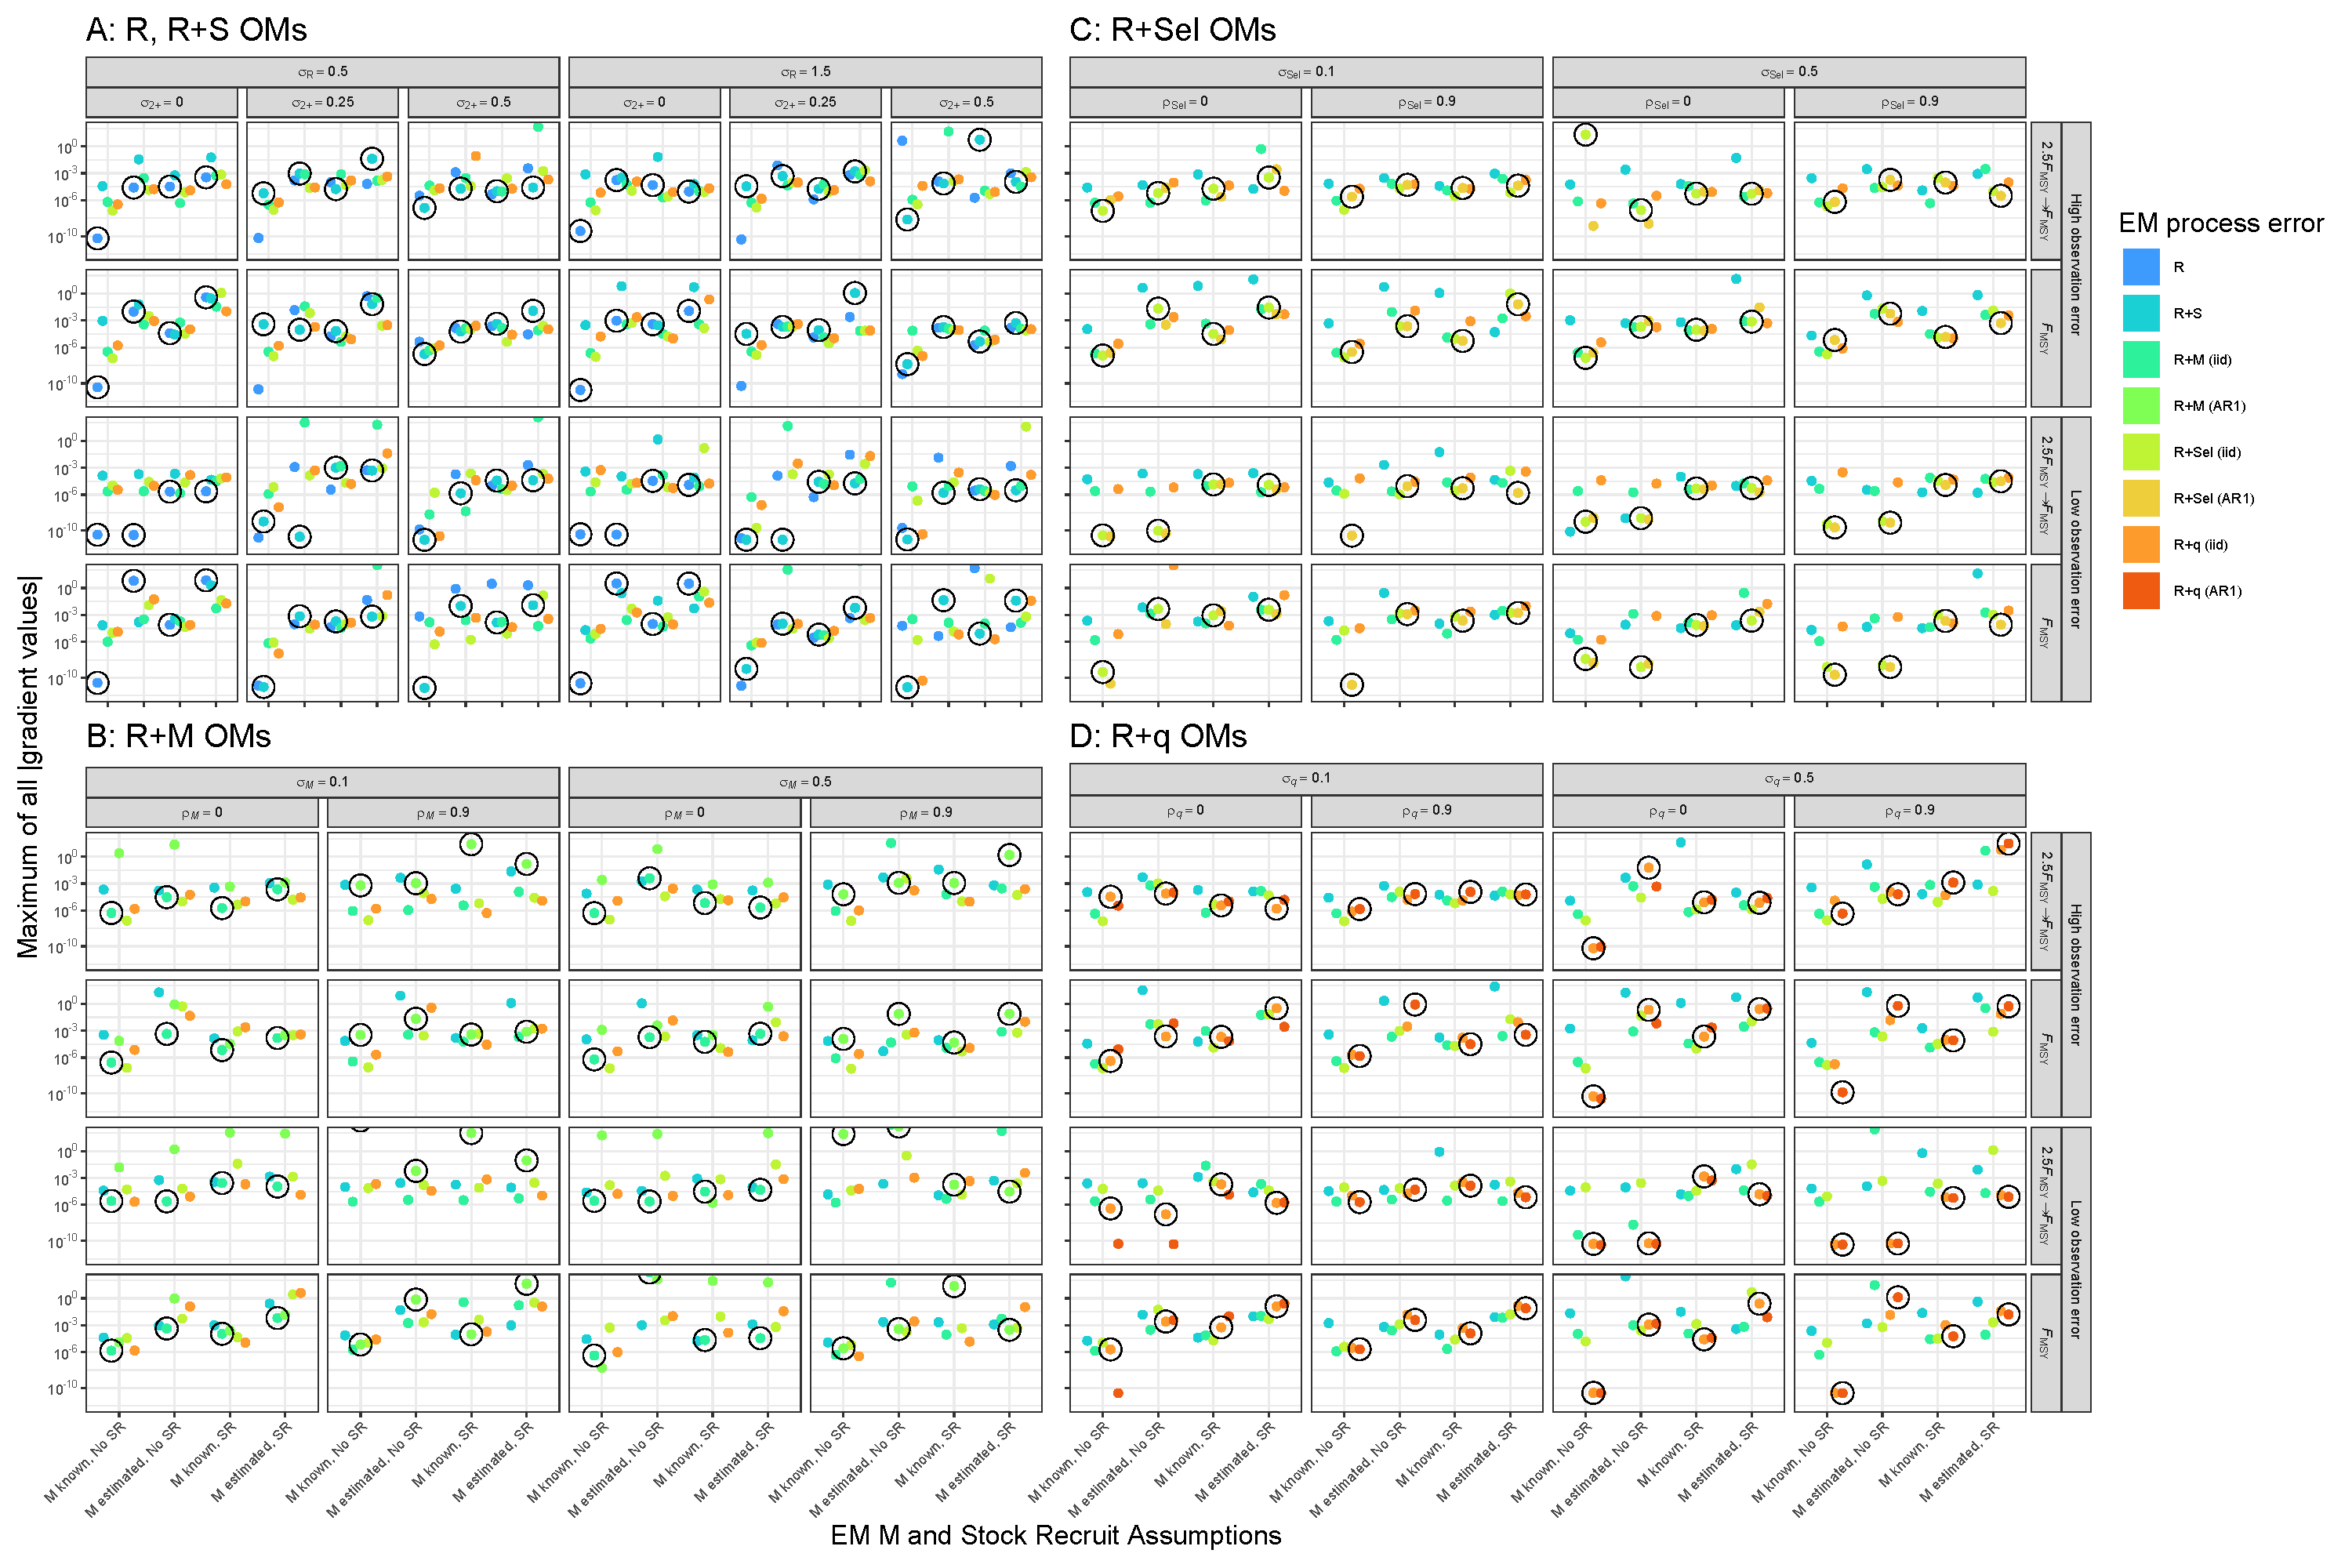
\includegraphics{hess_grad_convergence_plots}
\end{center}
\caption{The maximum of the absolute values of all gradient values for all fits that provided hessian-based standard errors across all simuated data sets of a given OM configuration (A: R and R+S, B: R+M, C: R+Sel, or D: R+q).  Results are conditional on EM fits with alternative process error type (colored points and lines), median natural mortality (estimated or known) and recruitment assumptions (Beverton-Holt stock recruit or not). Circled values indicate results where the EM process error structure matches that of the operating model and vertical lines represent 95\% confidence intervals.}\label{hess_grad}
\end{figure}
\end{landscape}

\begin{landscape}
\begin{figure}
\begin{center}
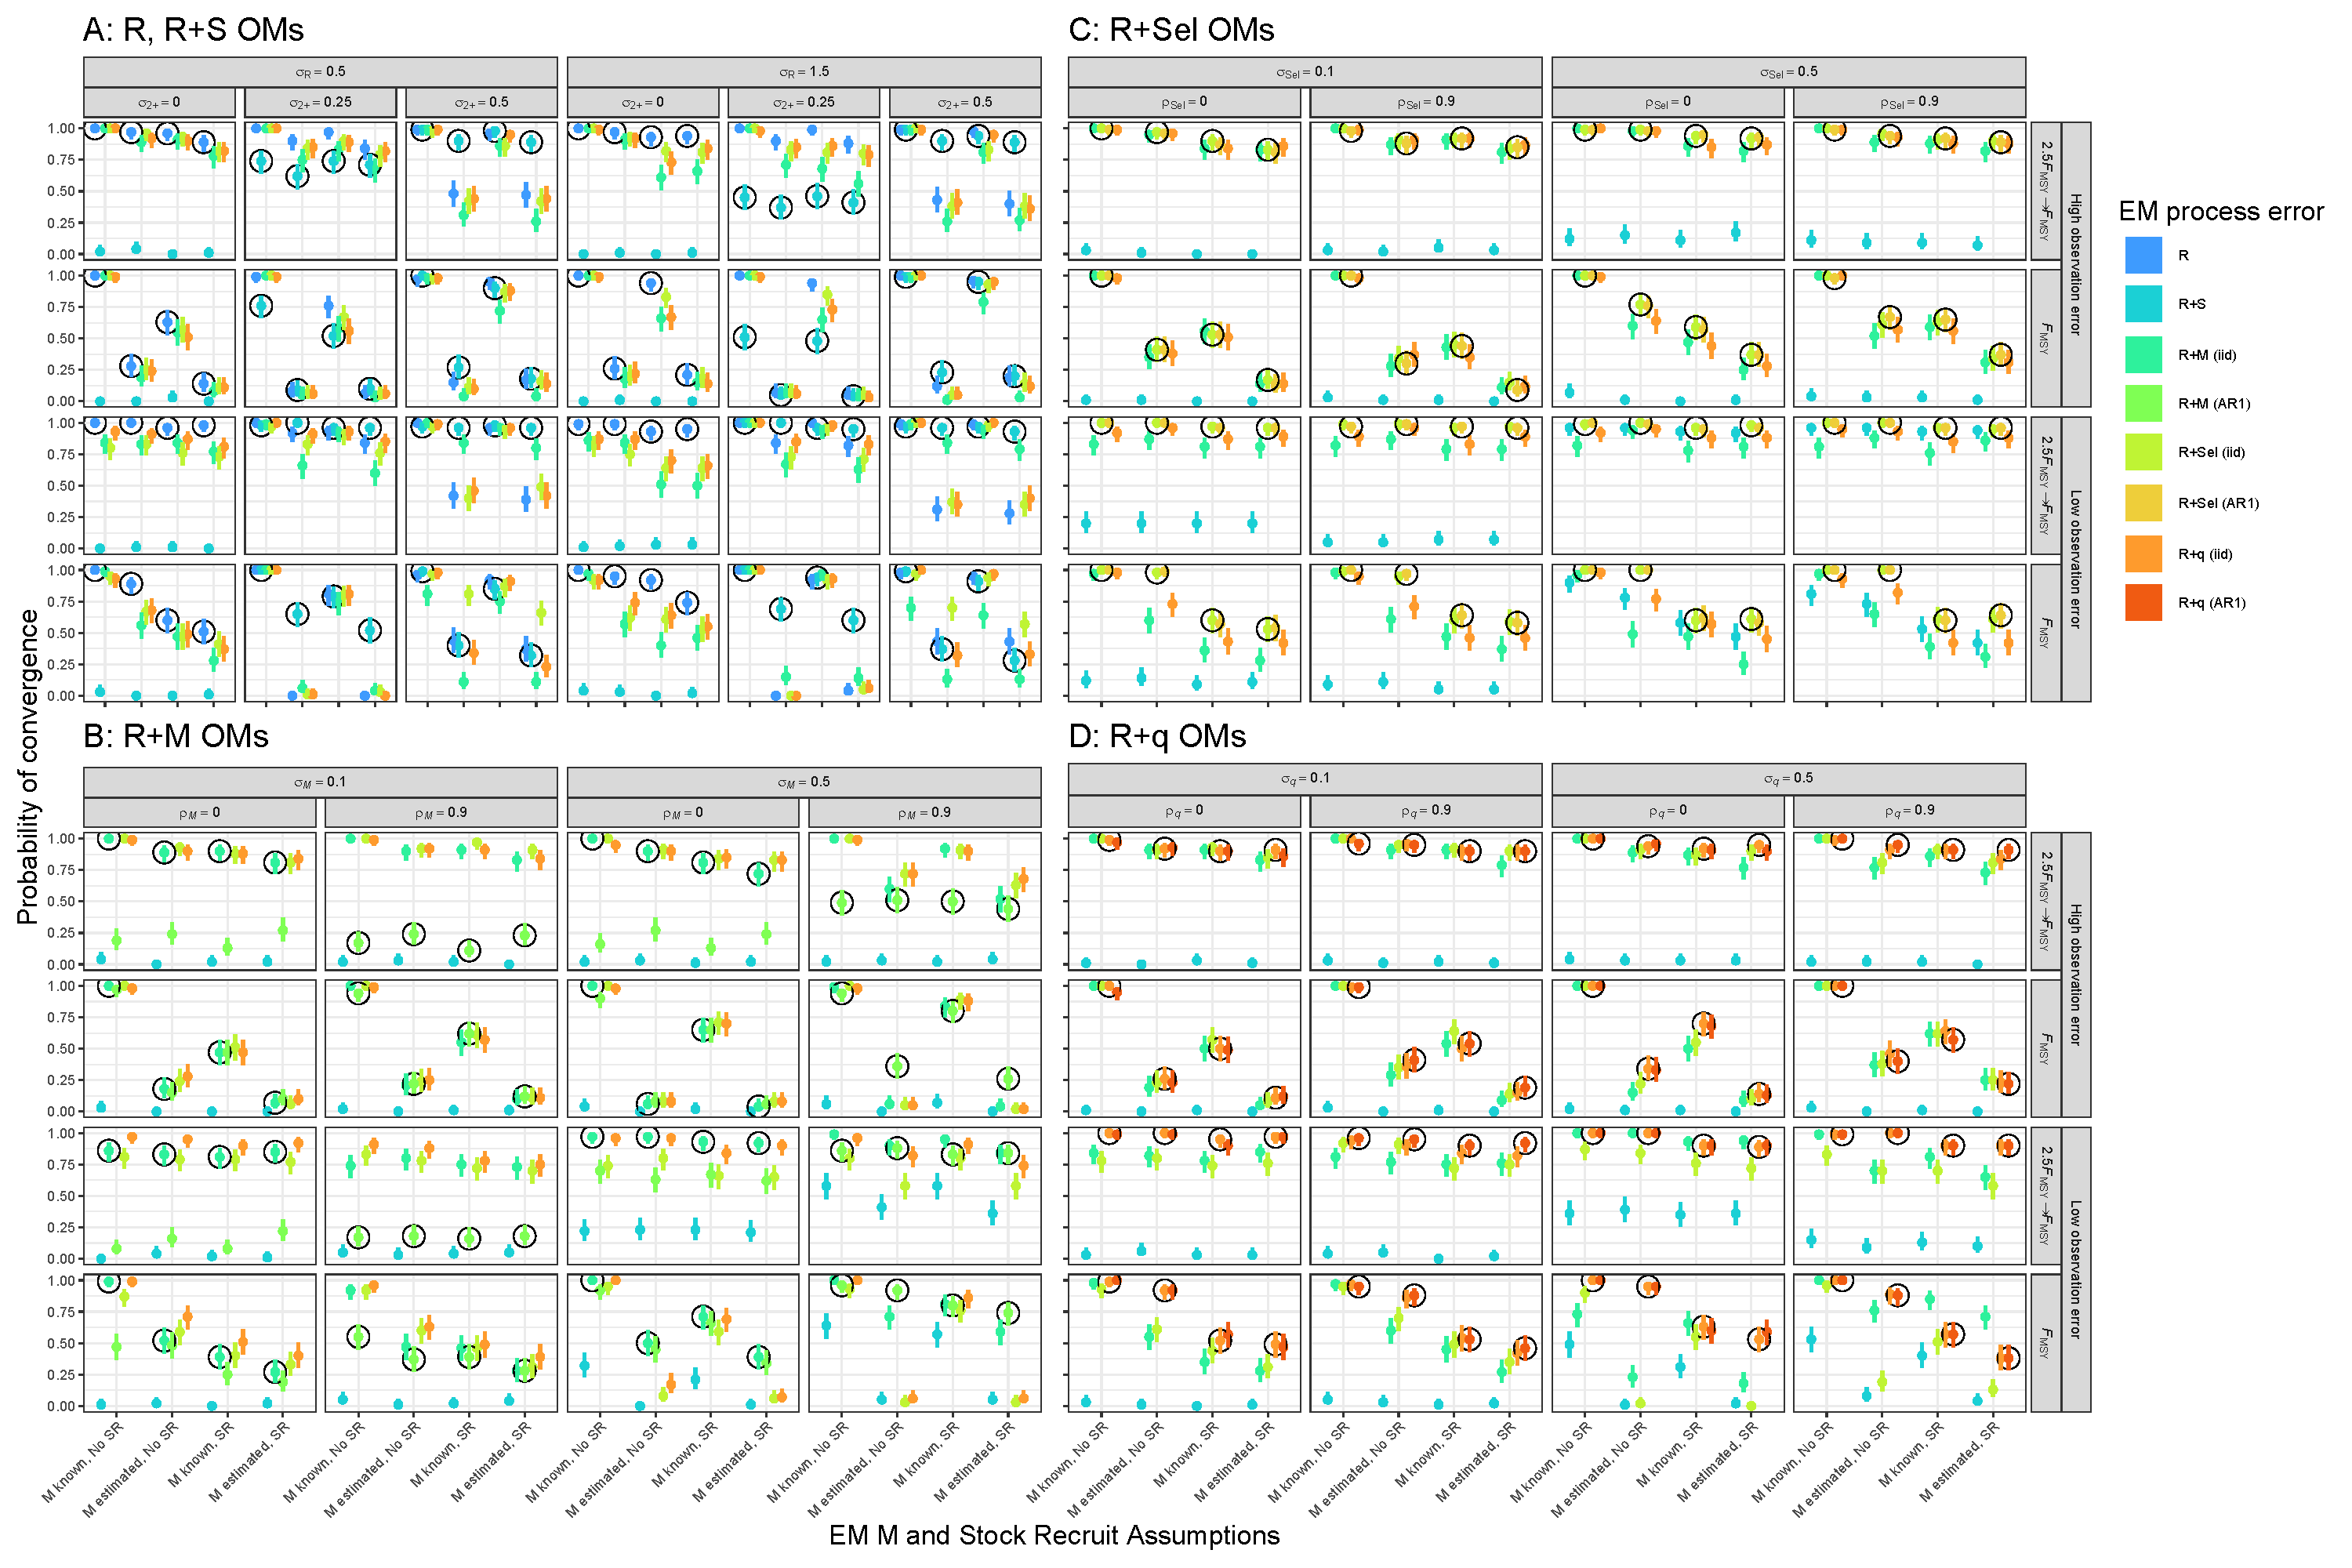
\includegraphics{type_3_convergence_plots}
\end{center}
\caption{Probability of estimating models providing maximum absolute values of gradients less than $10^{-6}$ assuming alternative process error (colored points and lines), and median natural mortality (estimated or known) and Beverton-Holt stock recruit functions (estimated or not; along x-axis) when fitted to operating models that have R and R+S (A), R+Sel (B), R+M (C), or R+q (D) process error structures. Circled values indicate results where the EM process error structure matches that of the operating model and vertical lines represent 95\% confidence intervals.}\label{gradient_convergence}
\end{figure}
\end{landscape}

\clearpage

\begin{landscape}
\begin{figure}
\begin{center}
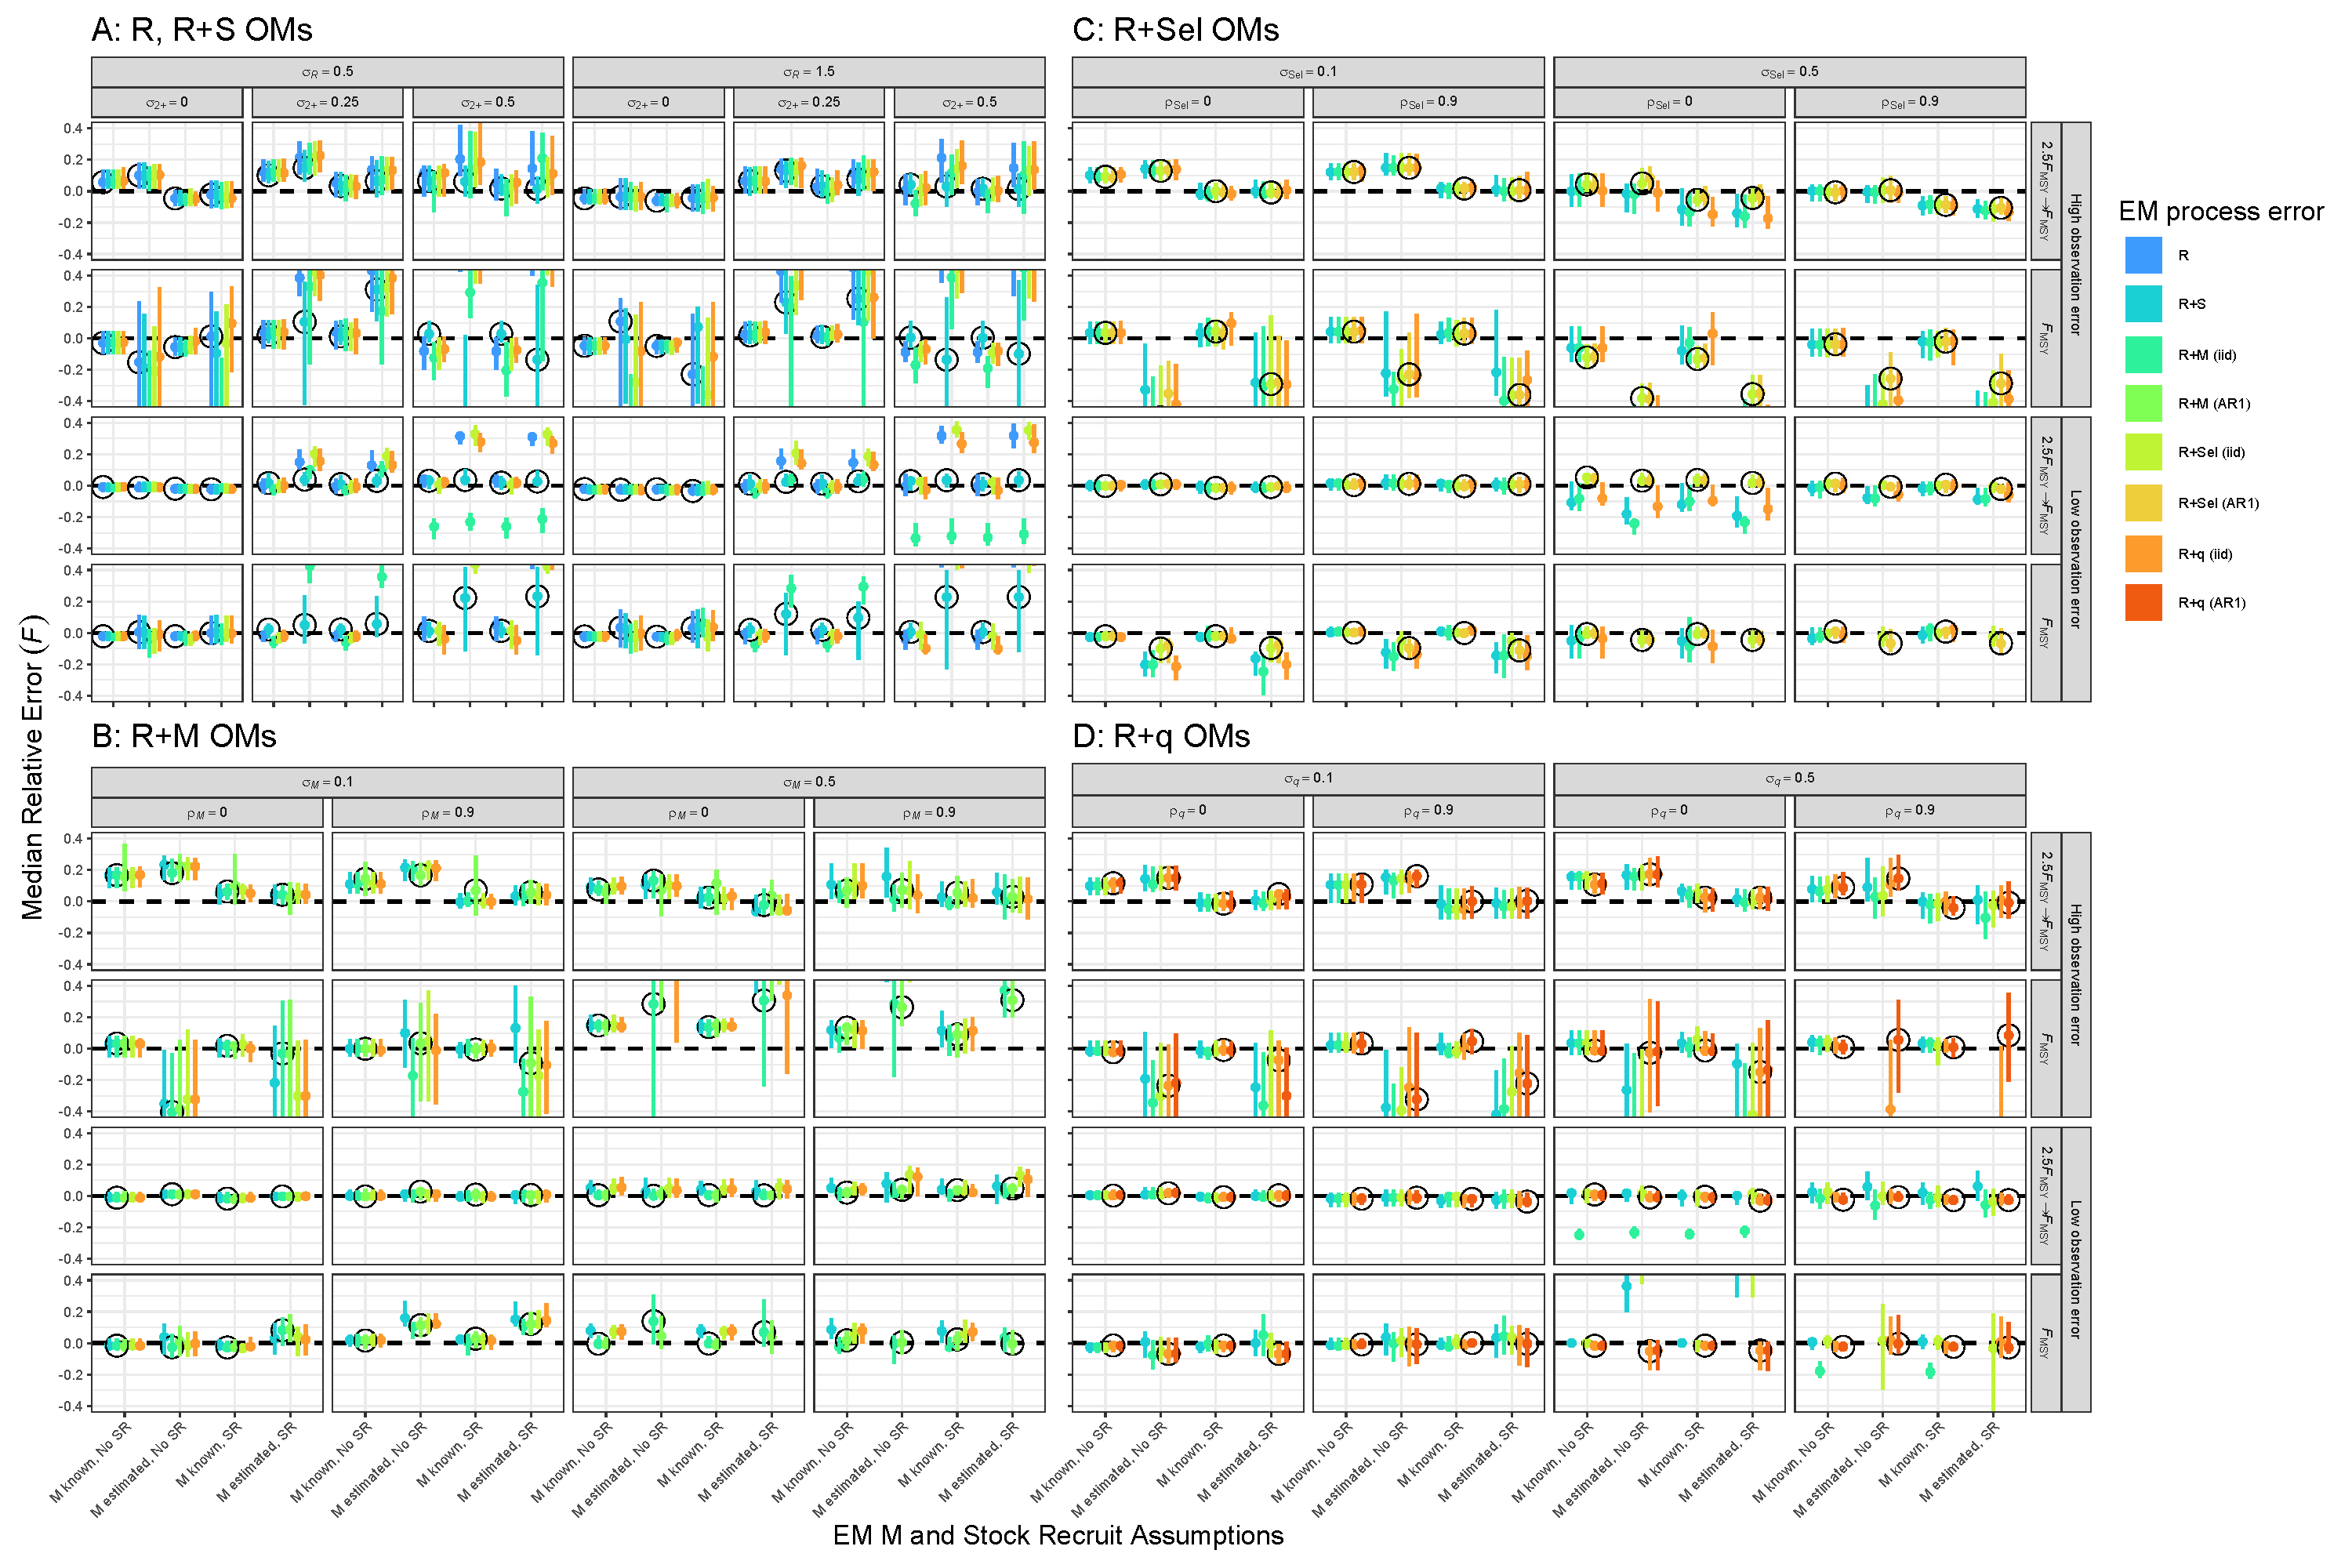
\includegraphics{term_F_bias_plots}
\end{center}
\caption{Median relative error of terminal year fully-selected fishing mortality for estimating models fitted to data sets simulated with alternative process error structures: R and R+S (A), R+Sel (B), R+M (C), or R+q (D). Circled values indicate results where the EM process error structure matches that of the operating model and vertical lines represent 95\% confidence intervals.}\label{F_rel_error}
\end{figure}
\end{landscape}

\begin{landscape}
\begin{figure}
\begin{center}
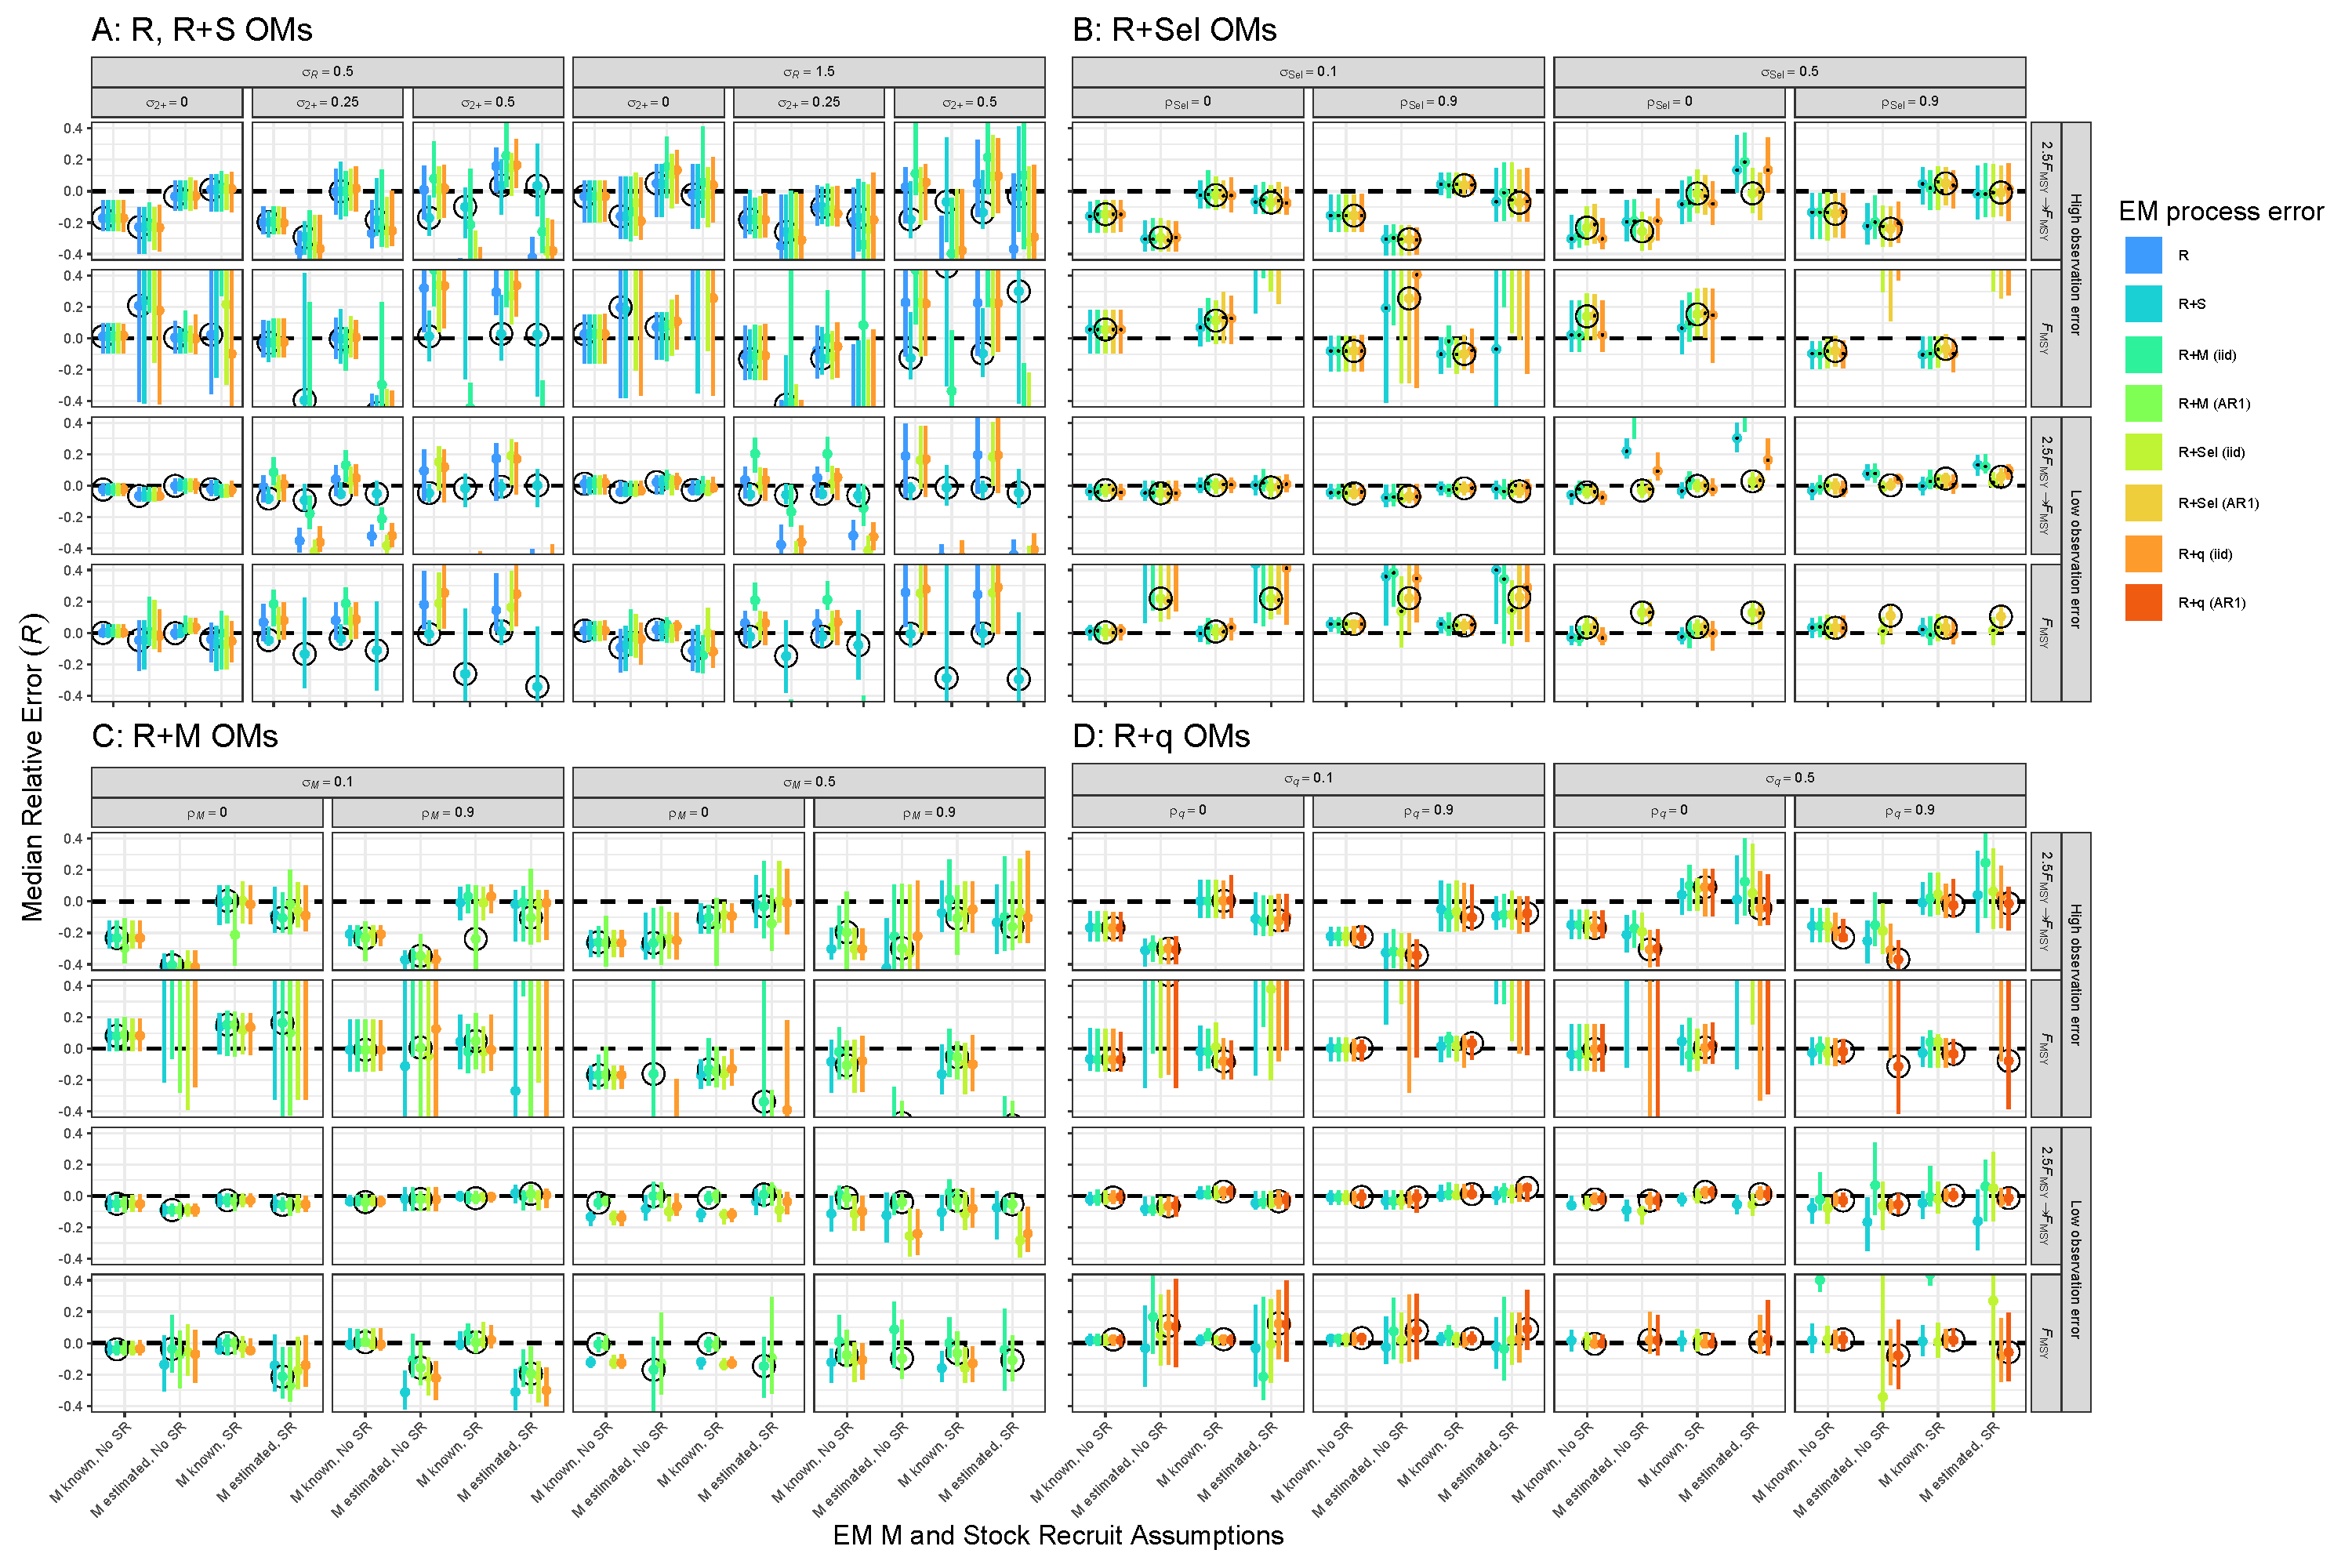
\includegraphics{term_R_bias_plots}
\end{center}
\caption{Median relative error of terminal year recruitment for estimating models fitted to data sets simulated with alternative process error structures: R and R+S (A), R+Sel (B), R+M (C), or R+q (D). Circled values indicate results where the EM process error structure matches that of the operating model and vertical lines represent 95\% confidence intervals.}\label{R_rel_error}
\end{figure}
\end{landscape}

\begin{landscape}
\begin{figure}
\begin{center}
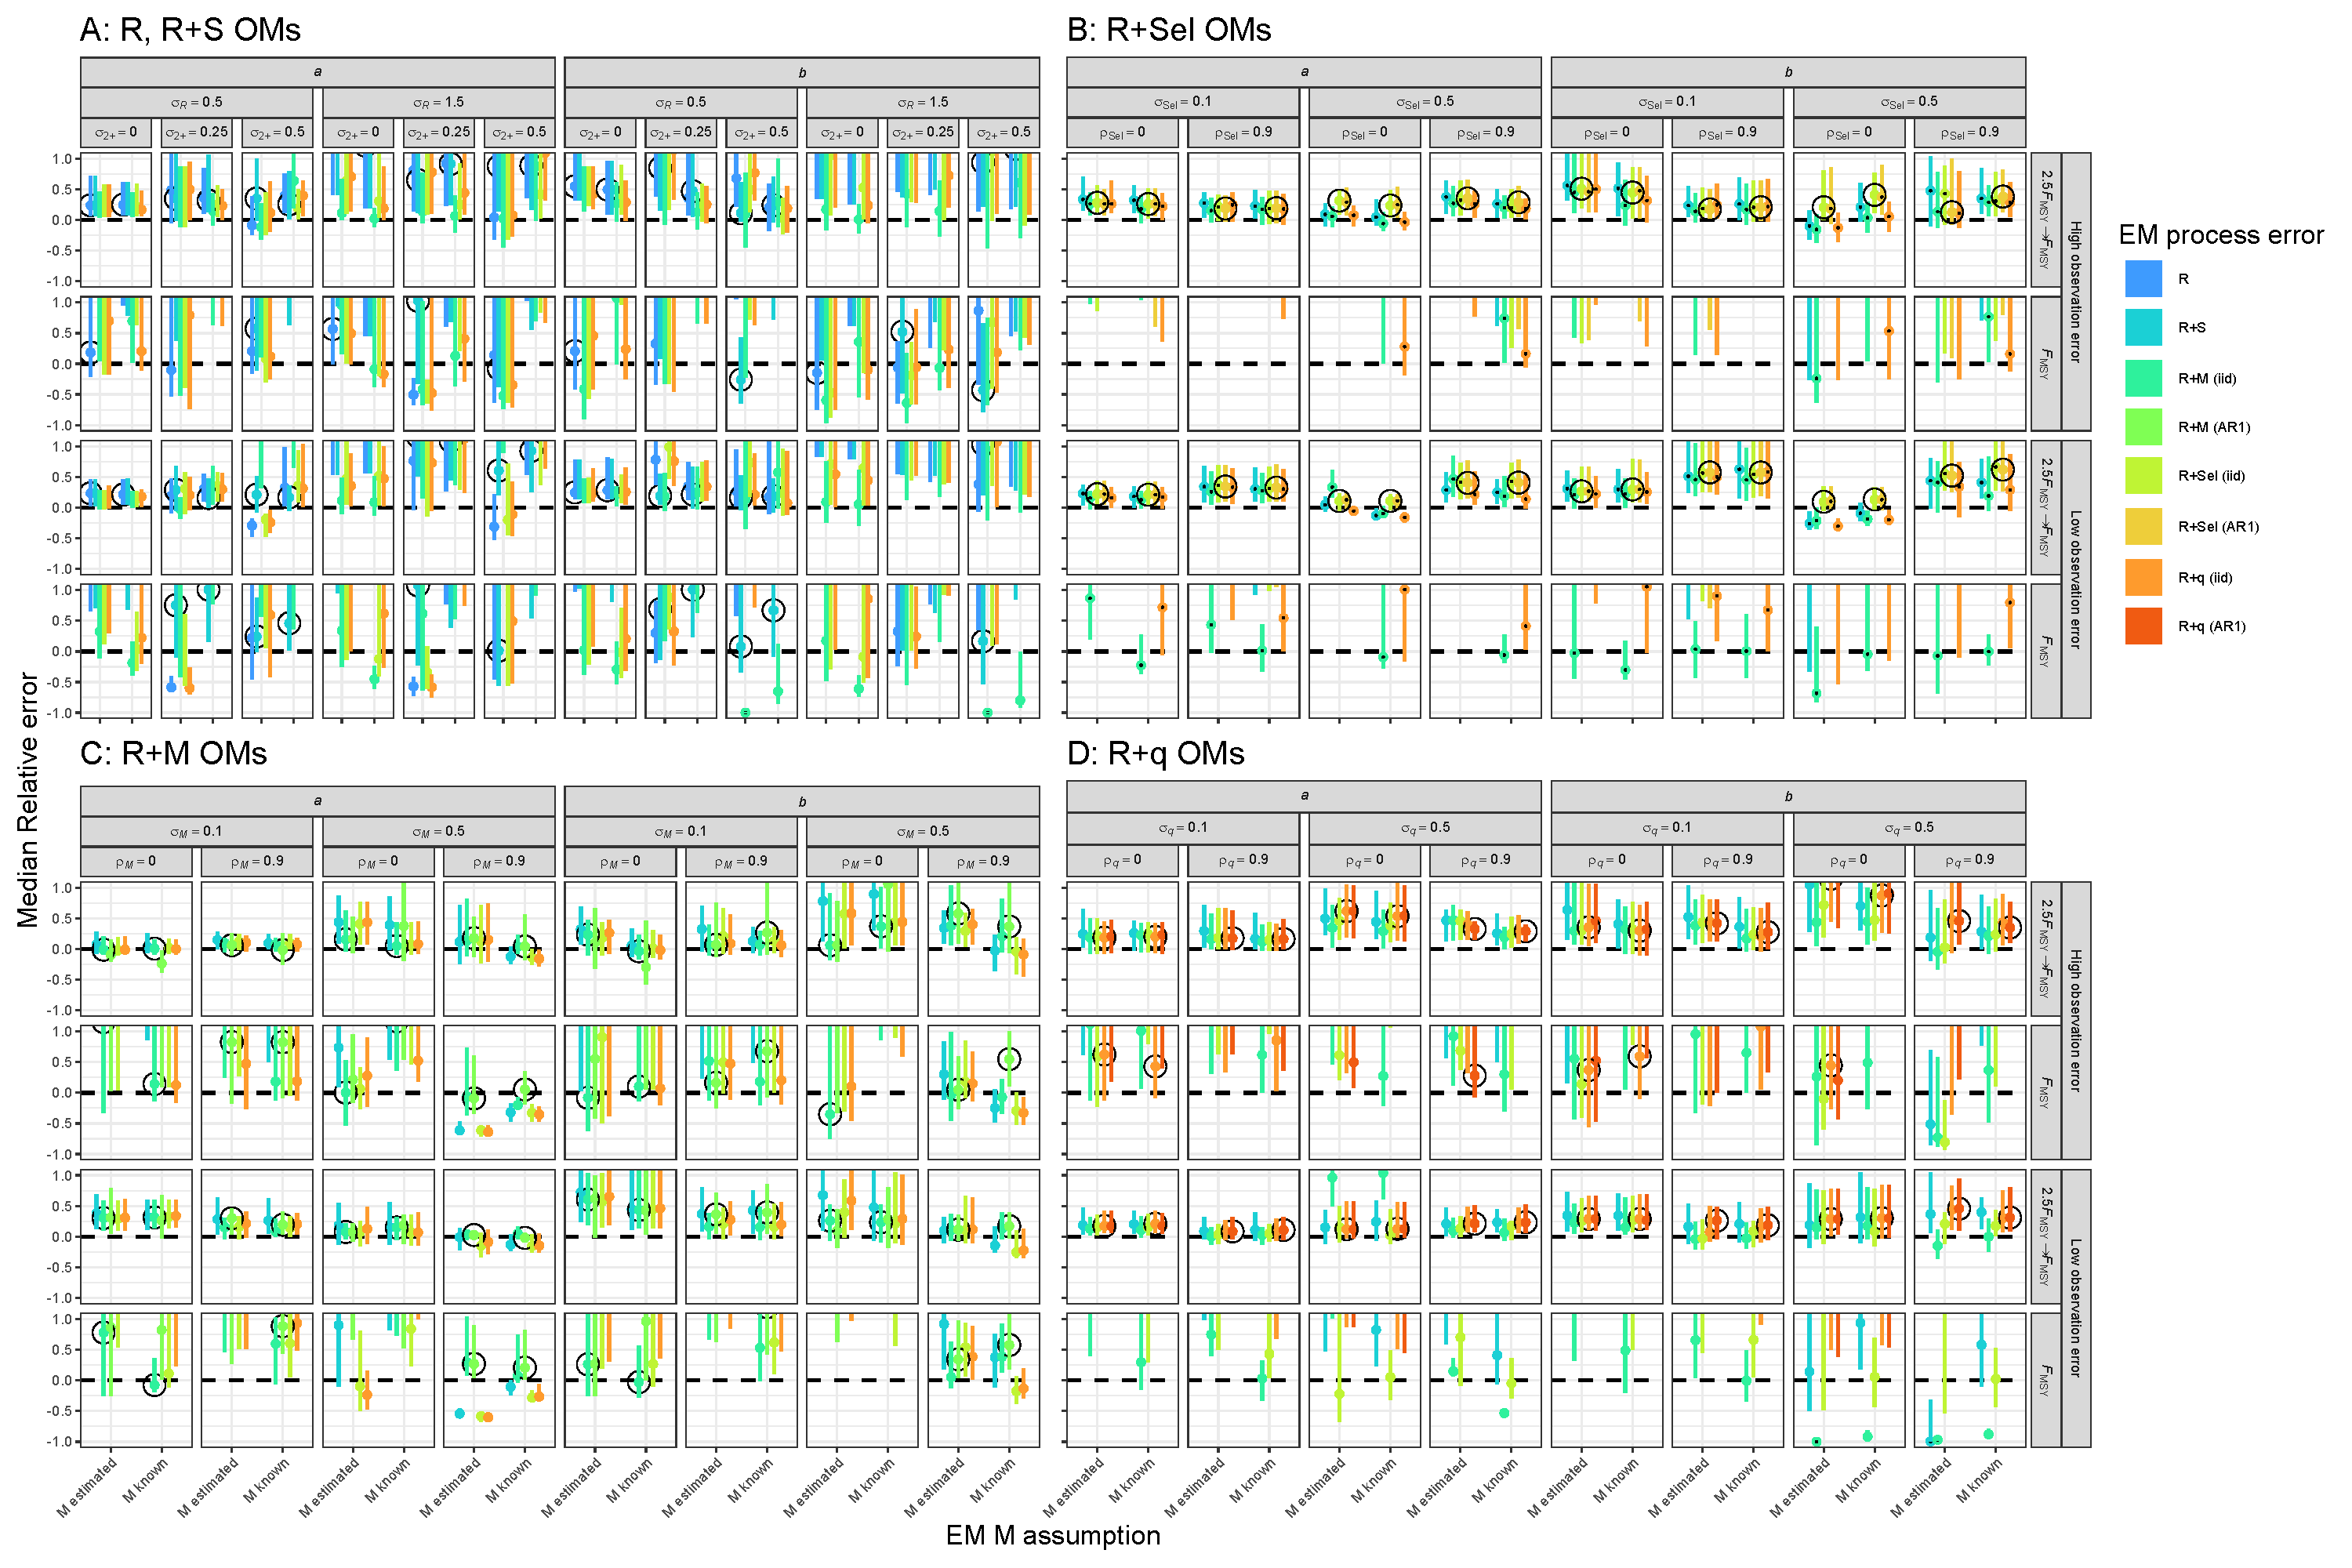
\includegraphics{sr_bias_plots}
\end{center}
\caption{Median relative error of Beverton-Holt stock recruitment parameters ($a$ and $b$) for estimating models fitted to data sets simulated with alternative process error structures: R and R+S (A), R+Sel (B), R+M (C), or R+q (D). Circled values indicate results where the EM process error structure matches that of the operating model and vertical lines represent 95\% confidence intervals.}\label{SR_rel_error}
\end{figure}
\end{landscape}

\begin{landscape}
\begin{figure}
\begin{center}
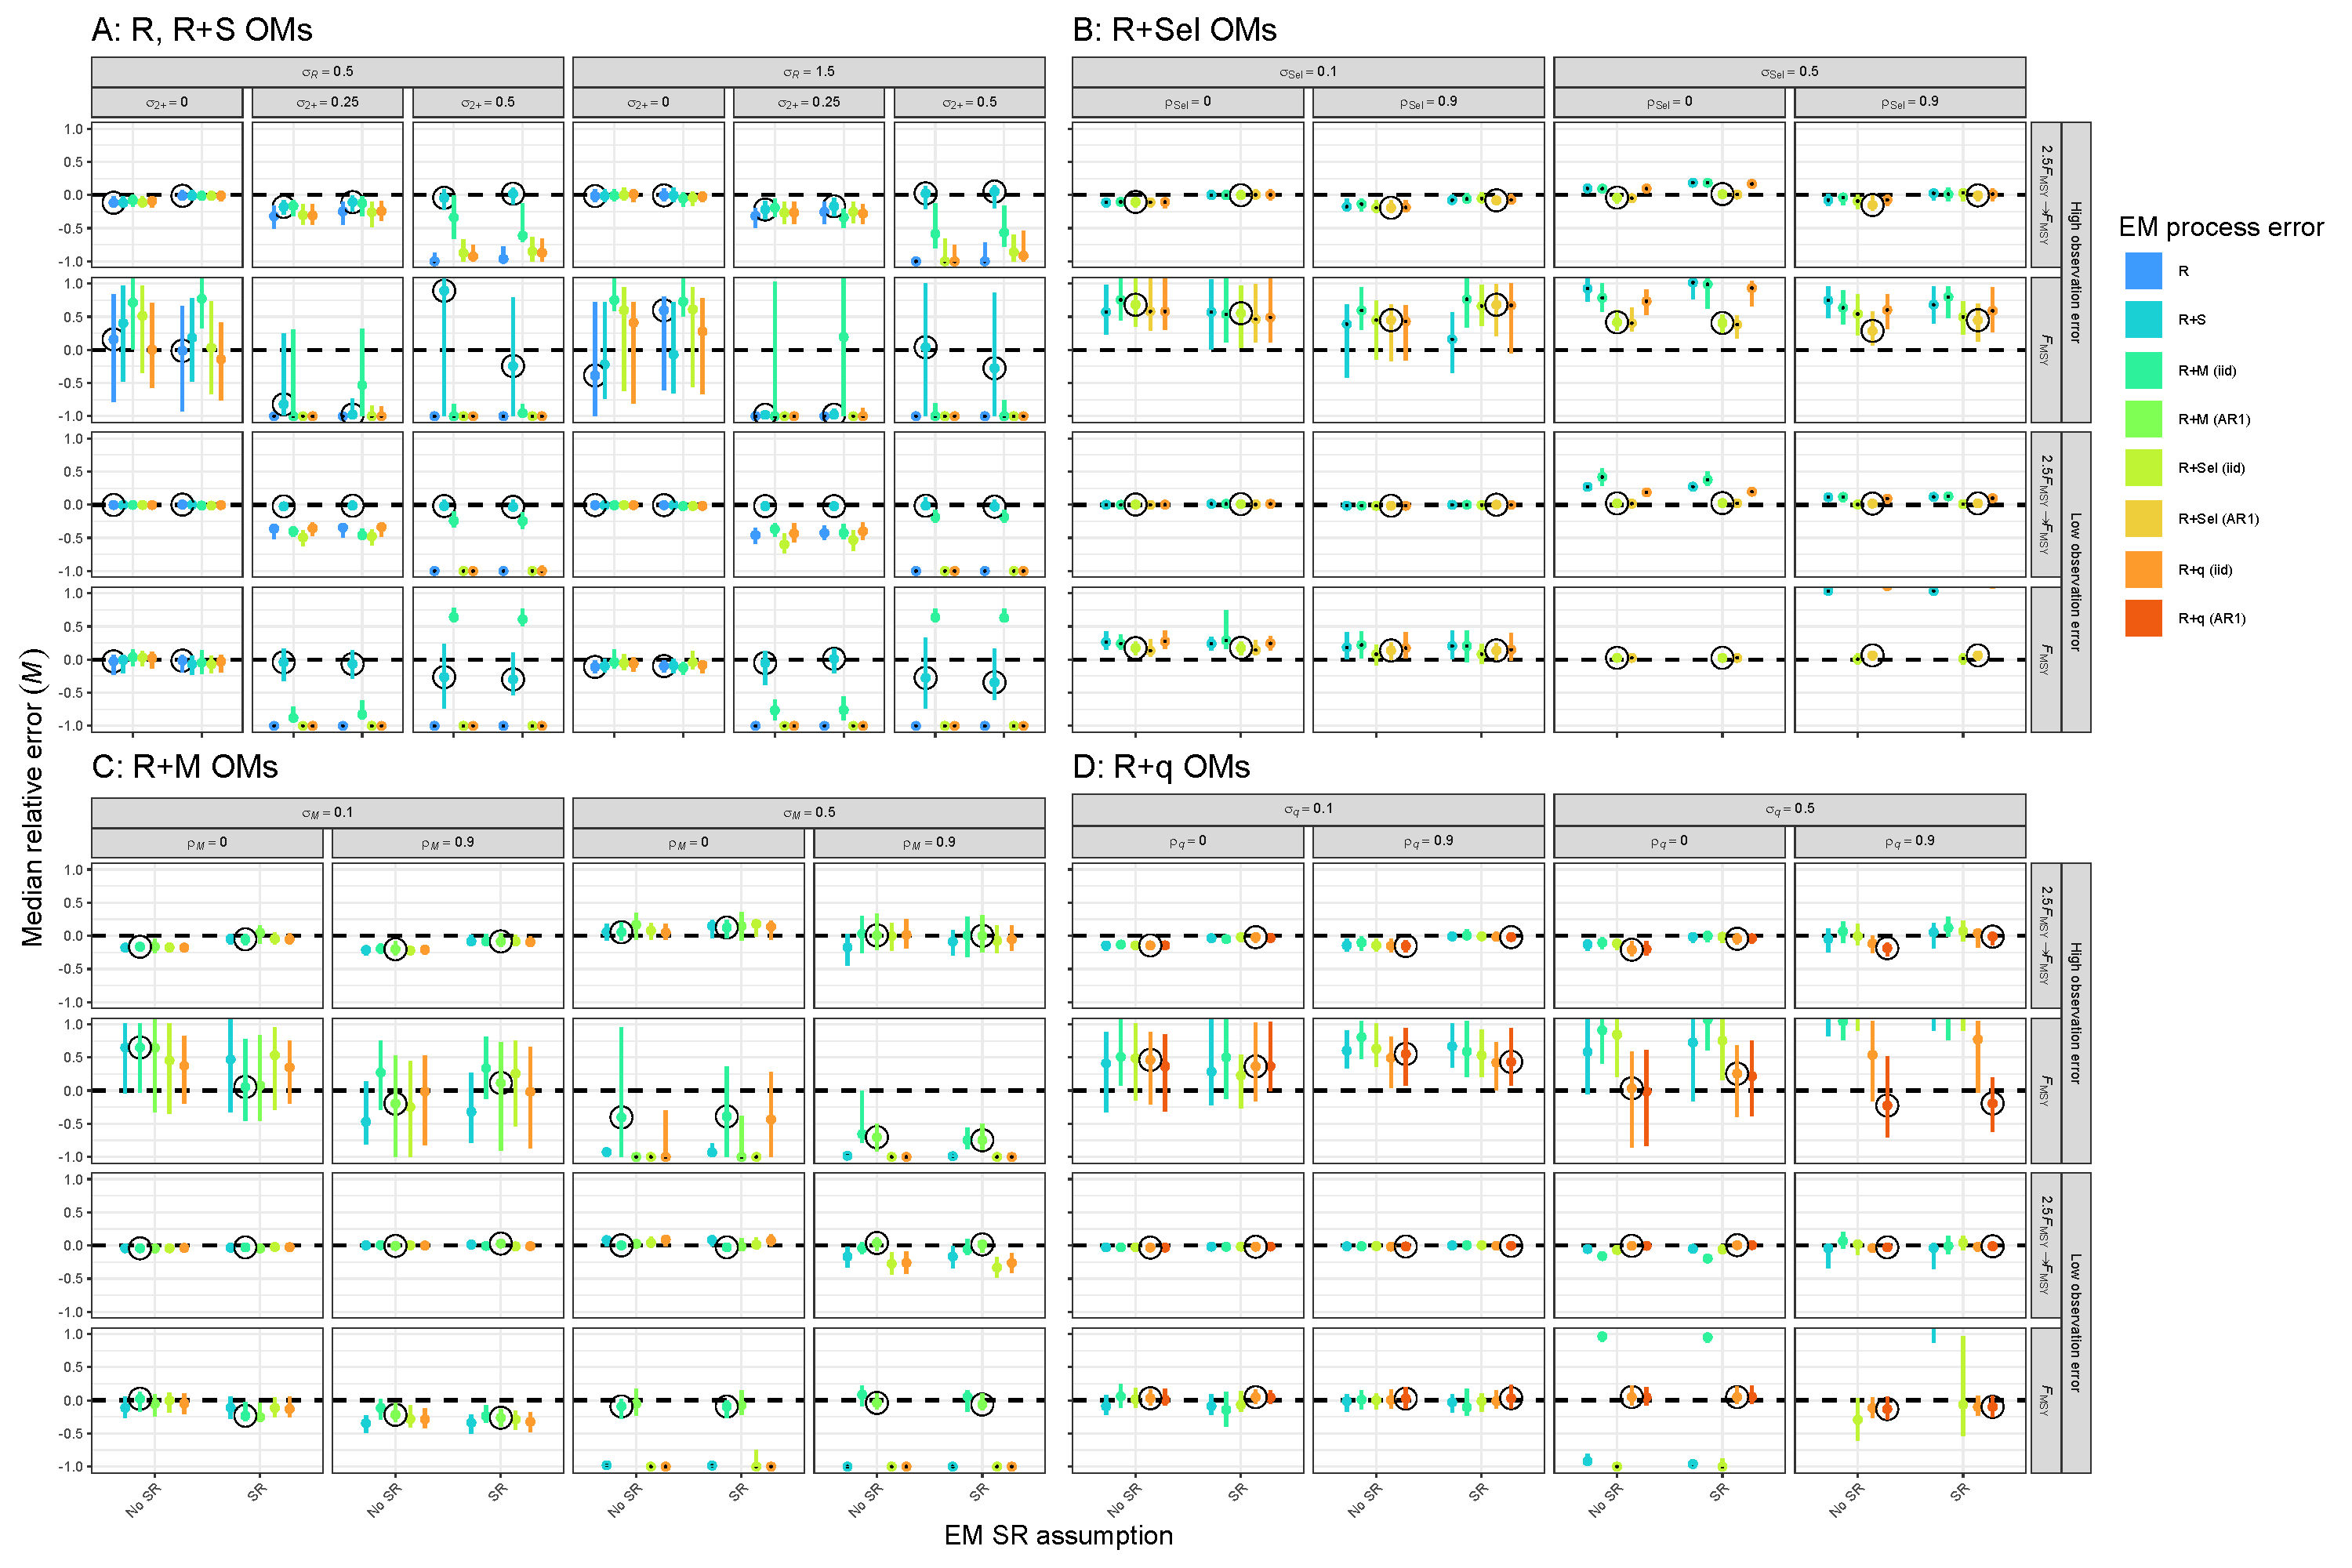
\includegraphics{M_bias_plots}
\end{center}
\caption{Median relative error of median natural mortality for estimating models fitted to data sets simulated with alternative process error structures: R and R+S (A), R+Sel (B), R+M (C), or R+q (D). Circled values indicate results where the EM process error structure matches that of the operating model and vertical lines represent 95\% confidence intervals.}\label{M_rel_error}
\end{figure}
\end{landscape}

\begin{landscape}
\begin{figure}
\begin{center}
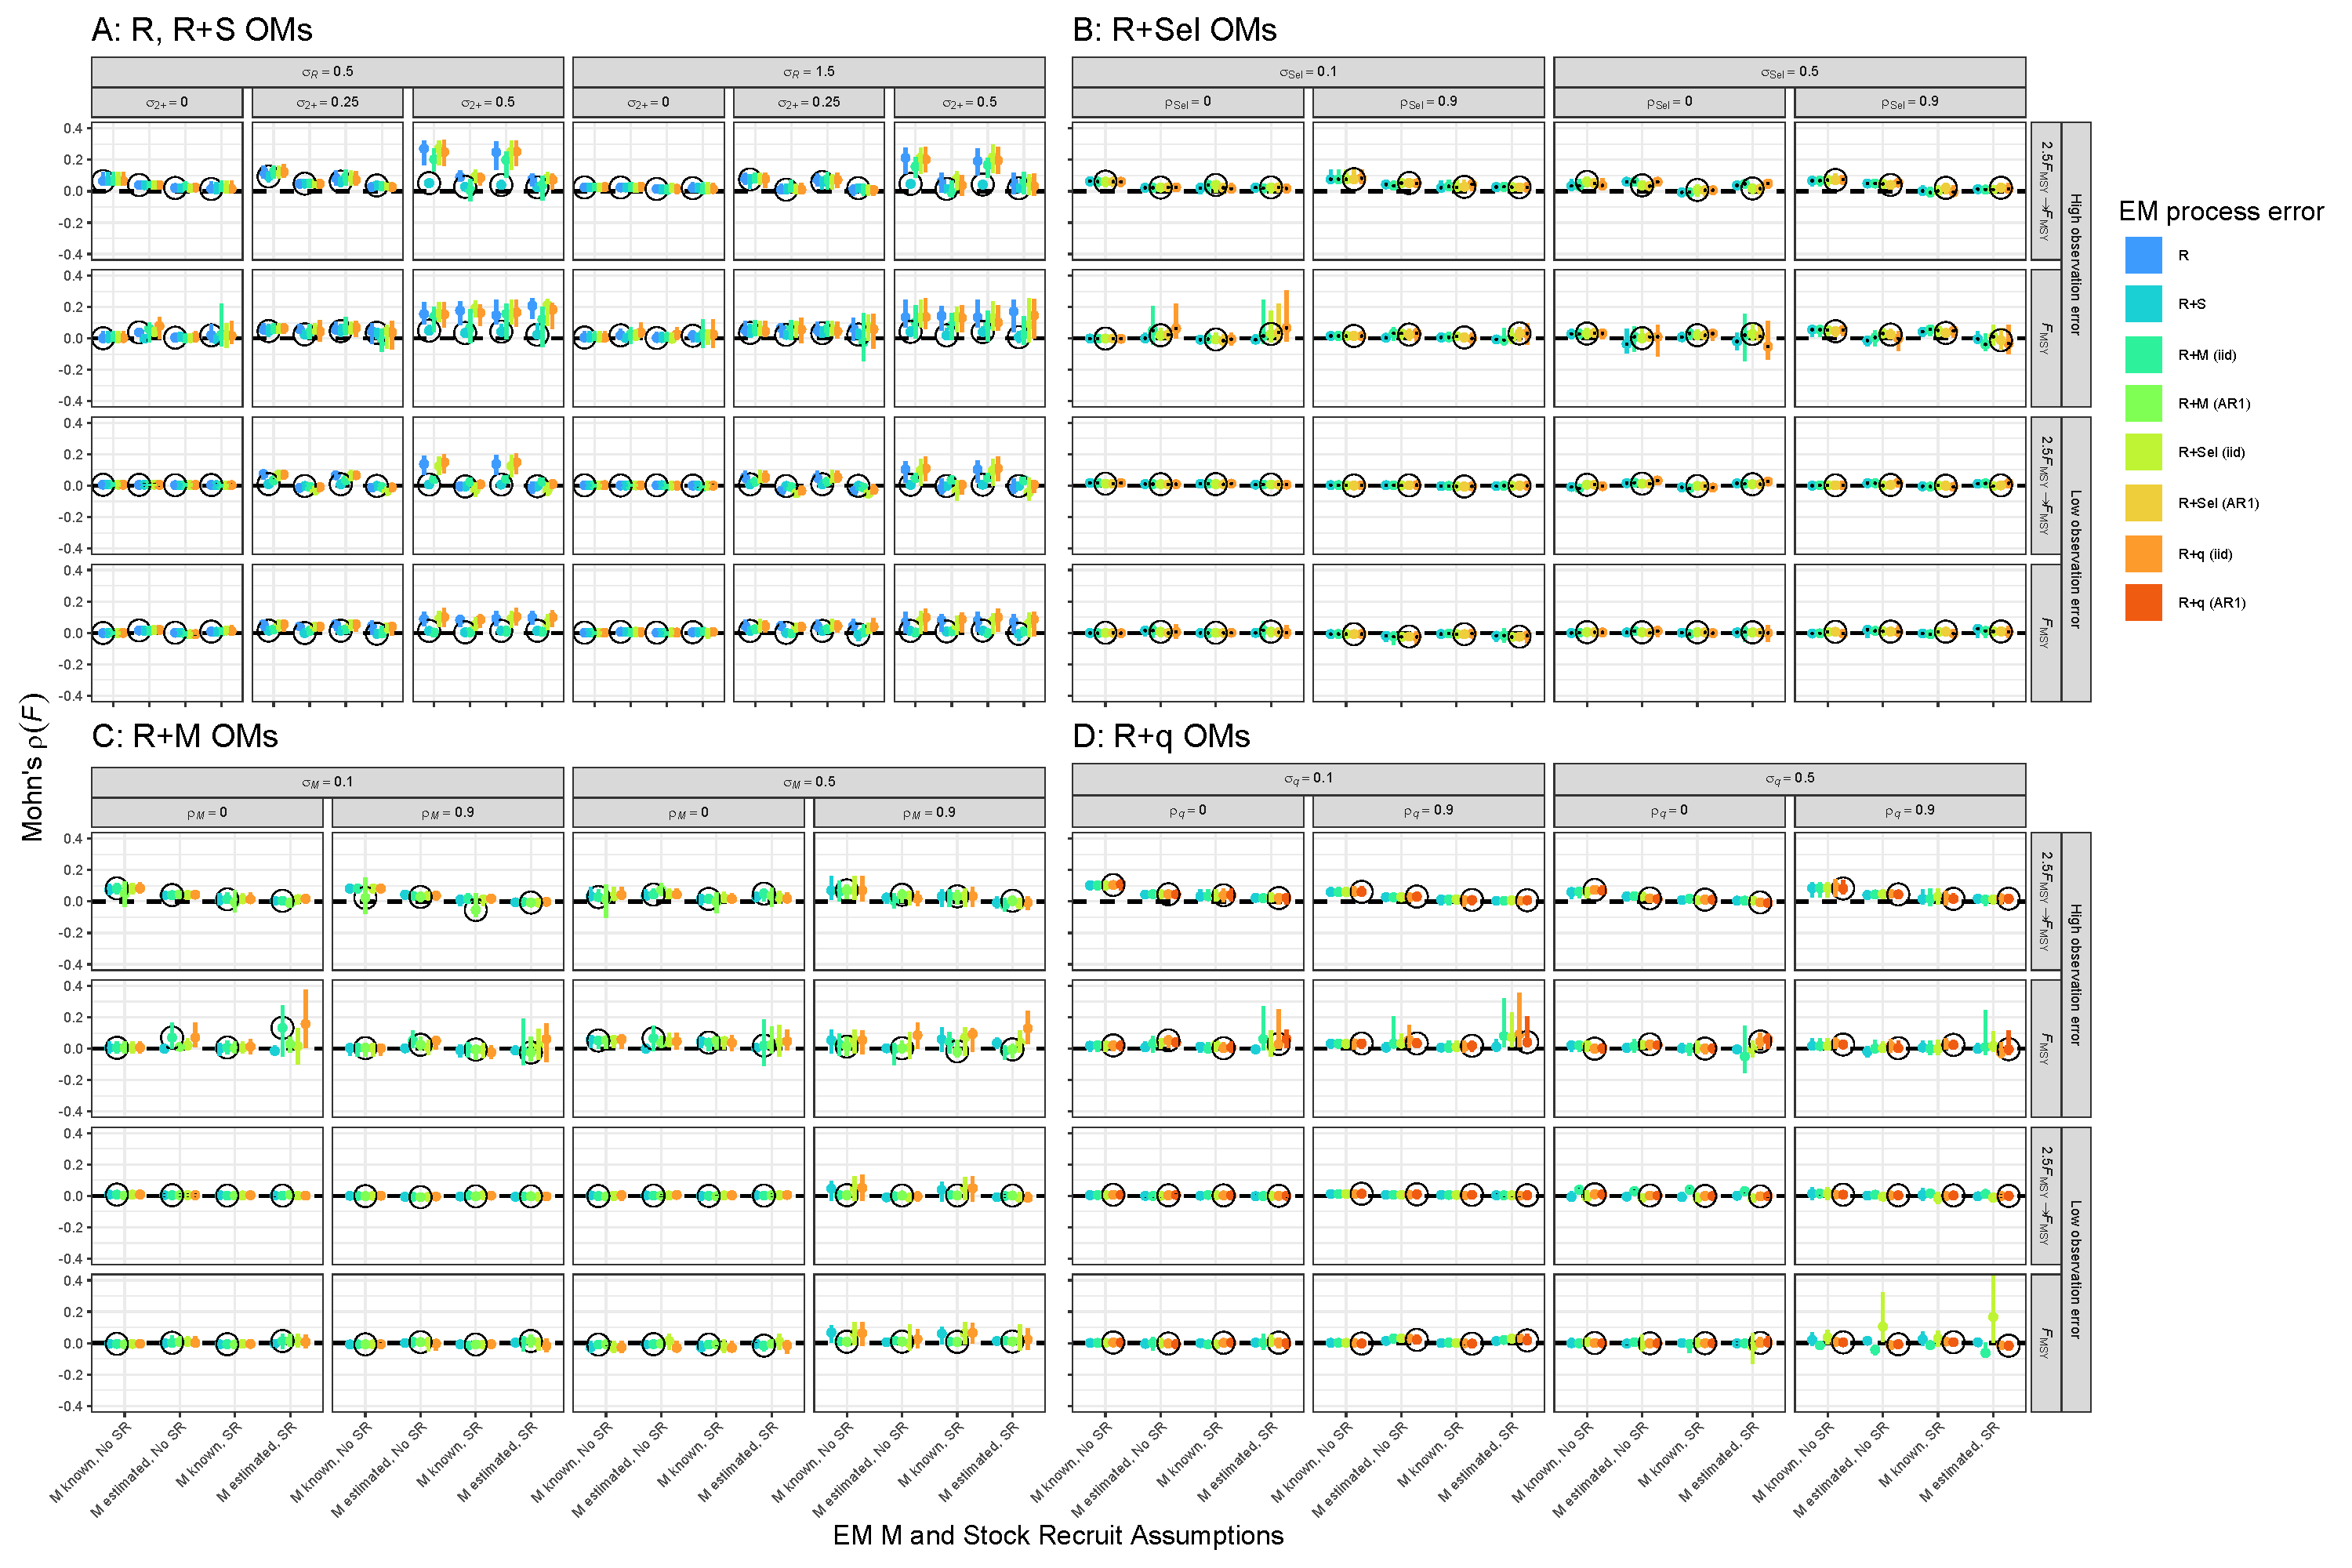
\includegraphics{mohns_rho_F_plots}
\end{center}
\caption{Median Mohn's $\rho$ of fishing mortality averaged over all age classes for estimating models fitted to data sets simulated with alternative process error structures: R and R+S (A), R+Sel (B), R+M (C), or R+q (D). Circled values indicate results where the EM process error structure matches that of the operating model and vertical lines represent 95\% confidence intervals.}\label{mohns_rho_F}
\end{figure}
\end{landscape}

\begin{landscape}
\begin{figure}
\begin{center}
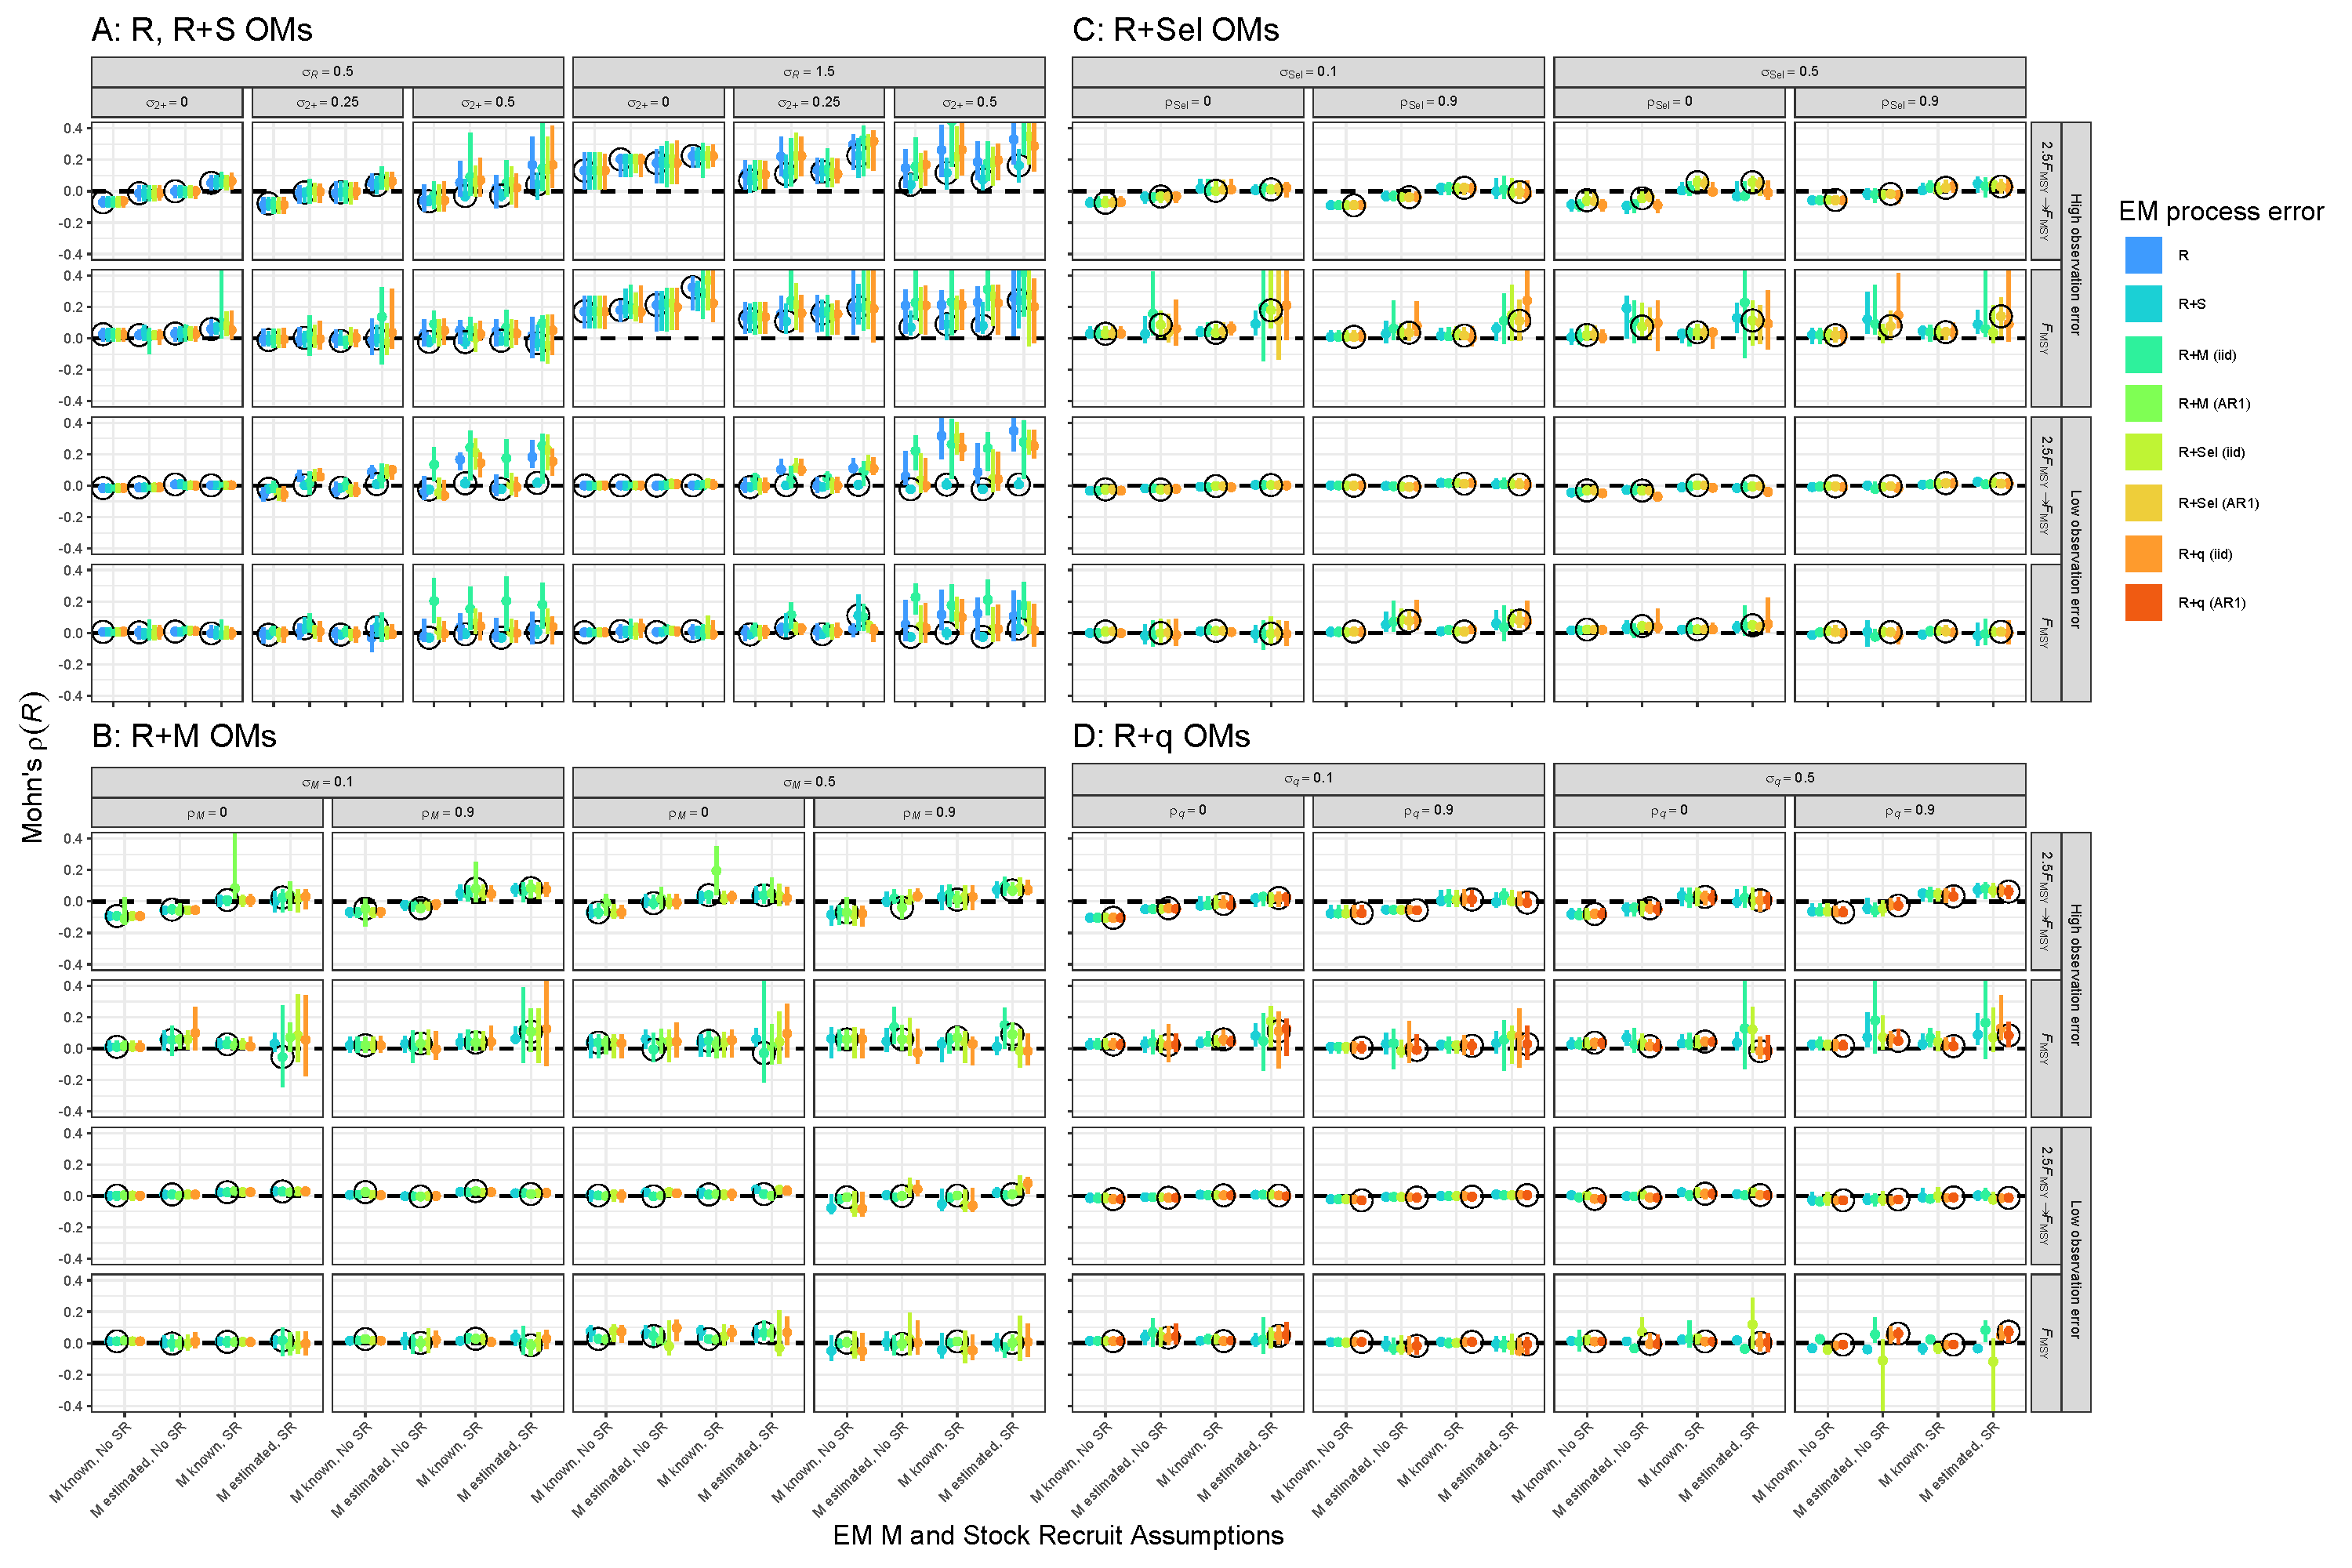
\includegraphics{mohns_rho_R_plots}
\end{center}
\caption{Median Mohn's $\rho$ of recruitment for estimating models fitted to data sets simulated with alternative process error structures: R and R+S (A), R+Sel (B), R+M (C), or R+q (D). Circled values indicate results where the EM process error structure matches that of the operating model and vertical lines represent 95\% confidence intervals.}\label{mohns_rho_R}
\end{figure}
\end{landscape}

\end{document}
